\chapter{Hardware implementation}\label{Hardware Implementation}
Here you show:
VHDL design
bit widths
latencies
signals
testbenches
block diagrams

\section{System overview}
\section{Data representation and scaling}

explain why  samples are in I/Q fxp, and testangles are cos/sin fxp (more difficult to calculate angles with,
easier to apply angles to samples)

% \section{Architecture}
% \subsection{Serialized blind phase search block}
% \subsubsection{Functional}
% The most fundamental functional block of the SBPS pipeline is the stage. A certain stage $ m $ refers to 
% the calculation of an output phase estimation $ \phi_m $ for a block input $ \bar r \in (r_0; r_{\cal W}) $ with a previous
% estimation of $ \phi_{m-1} $ on which the test-angles are generated.
% Multiple of these stages get chained together approach the middle-of-block phase estimation at the 
% output of the final stage.

% \begin{figure}[h]
% \centering
% 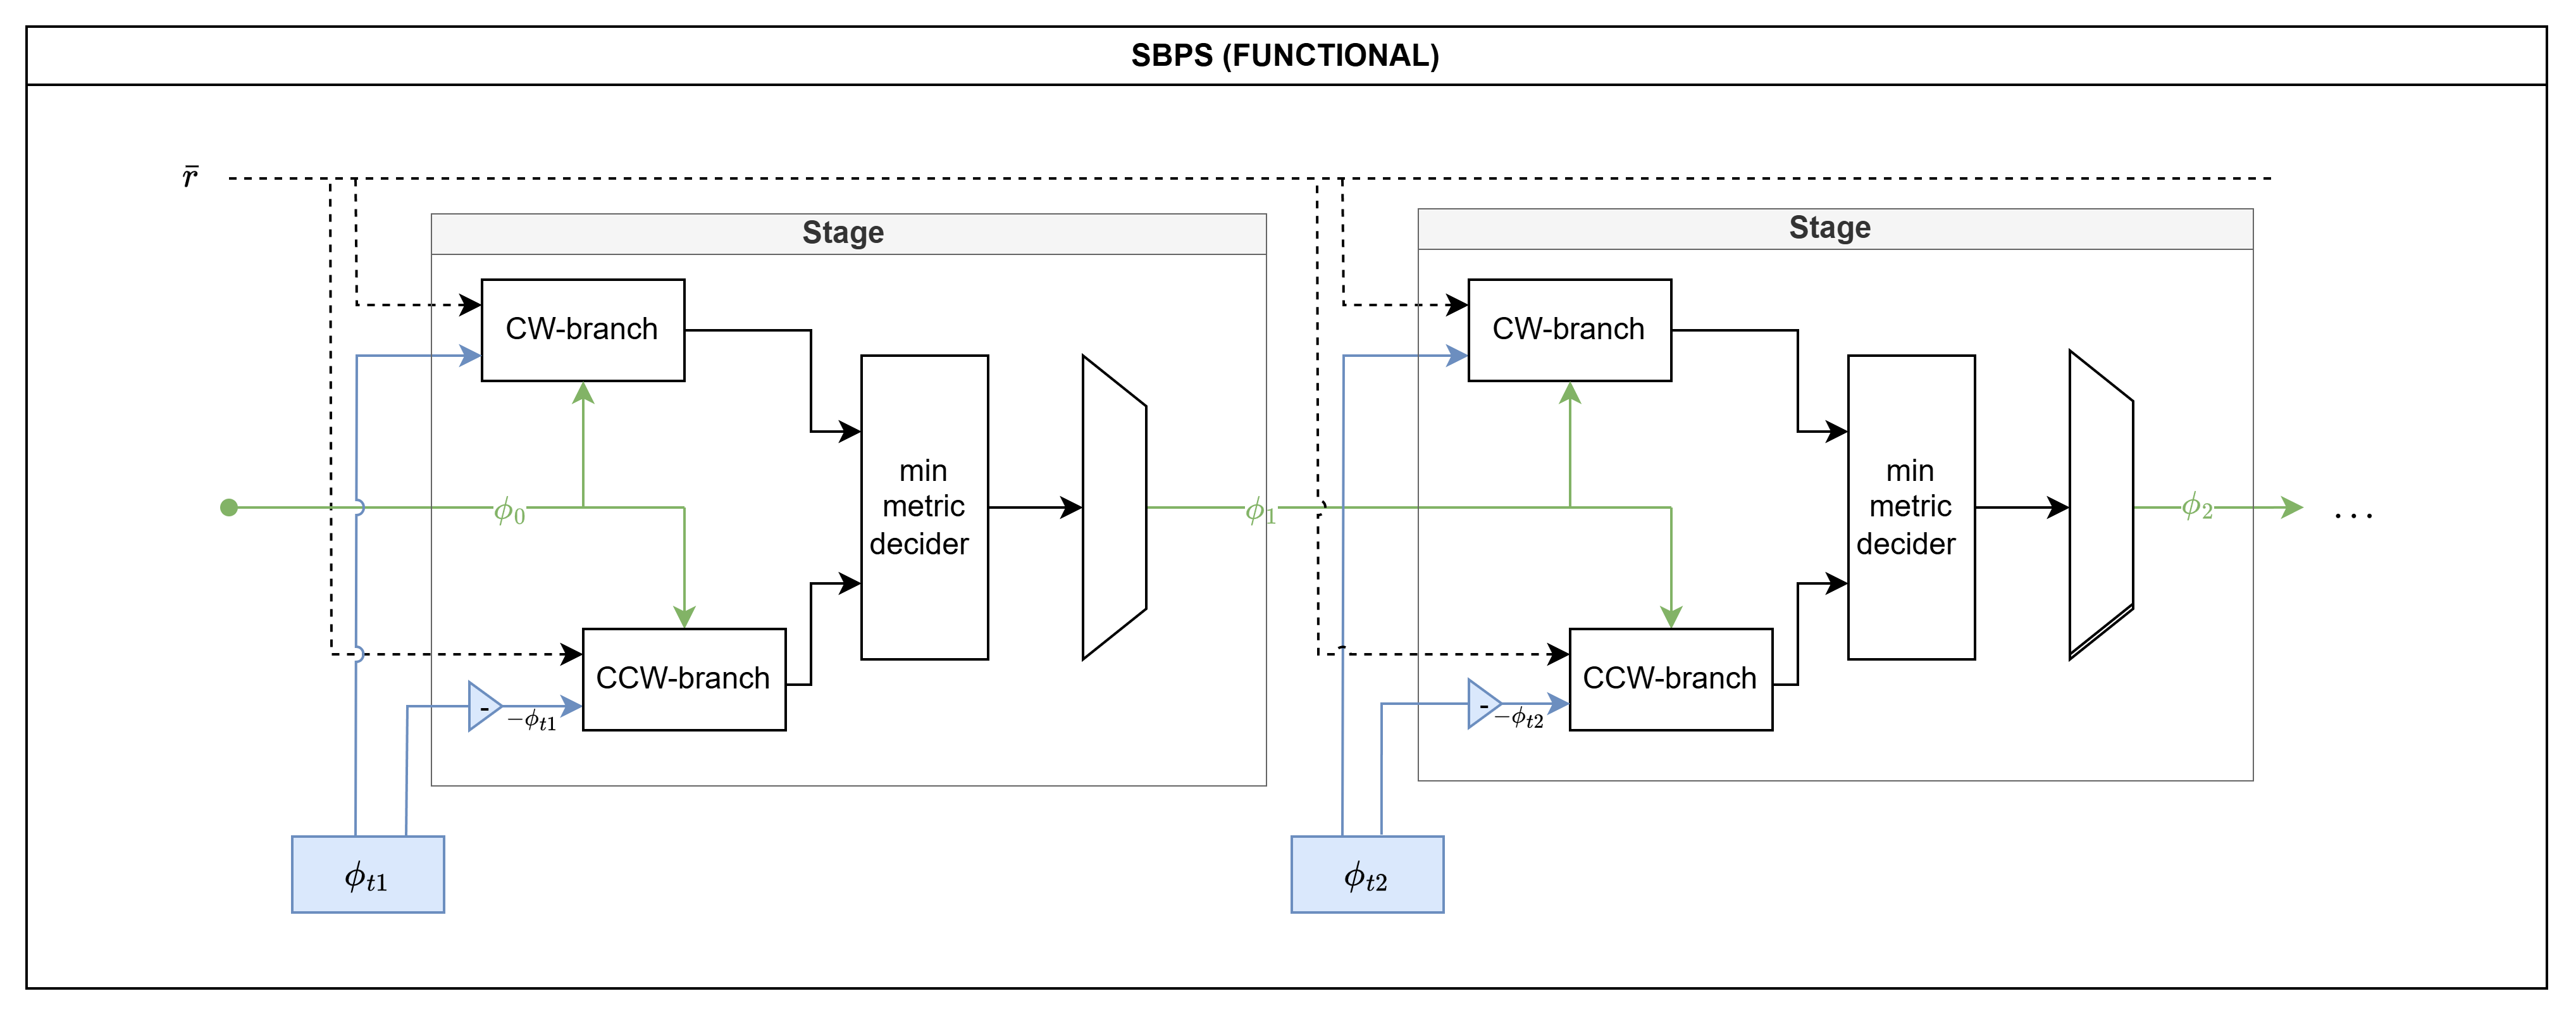
\includegraphics[width=1\linewidth]{figures/SBPS_functional.png}
% \caption{Functional diagram of the full SBPS architecture }
% \label{fig:functional-SBPS}
% \end{figure}

% The stage $ m $ decides wether the positive test-angle $ +\phi_t $ or negative test-angle $ -\phi_t $ should be added to the previous stage 
% phase estimation $ \phi_{m-1} $ to generate $ \phi_m $, 
% based on the error caused by the test-angle. 

% \begin{figure}[h]
% \centering
% 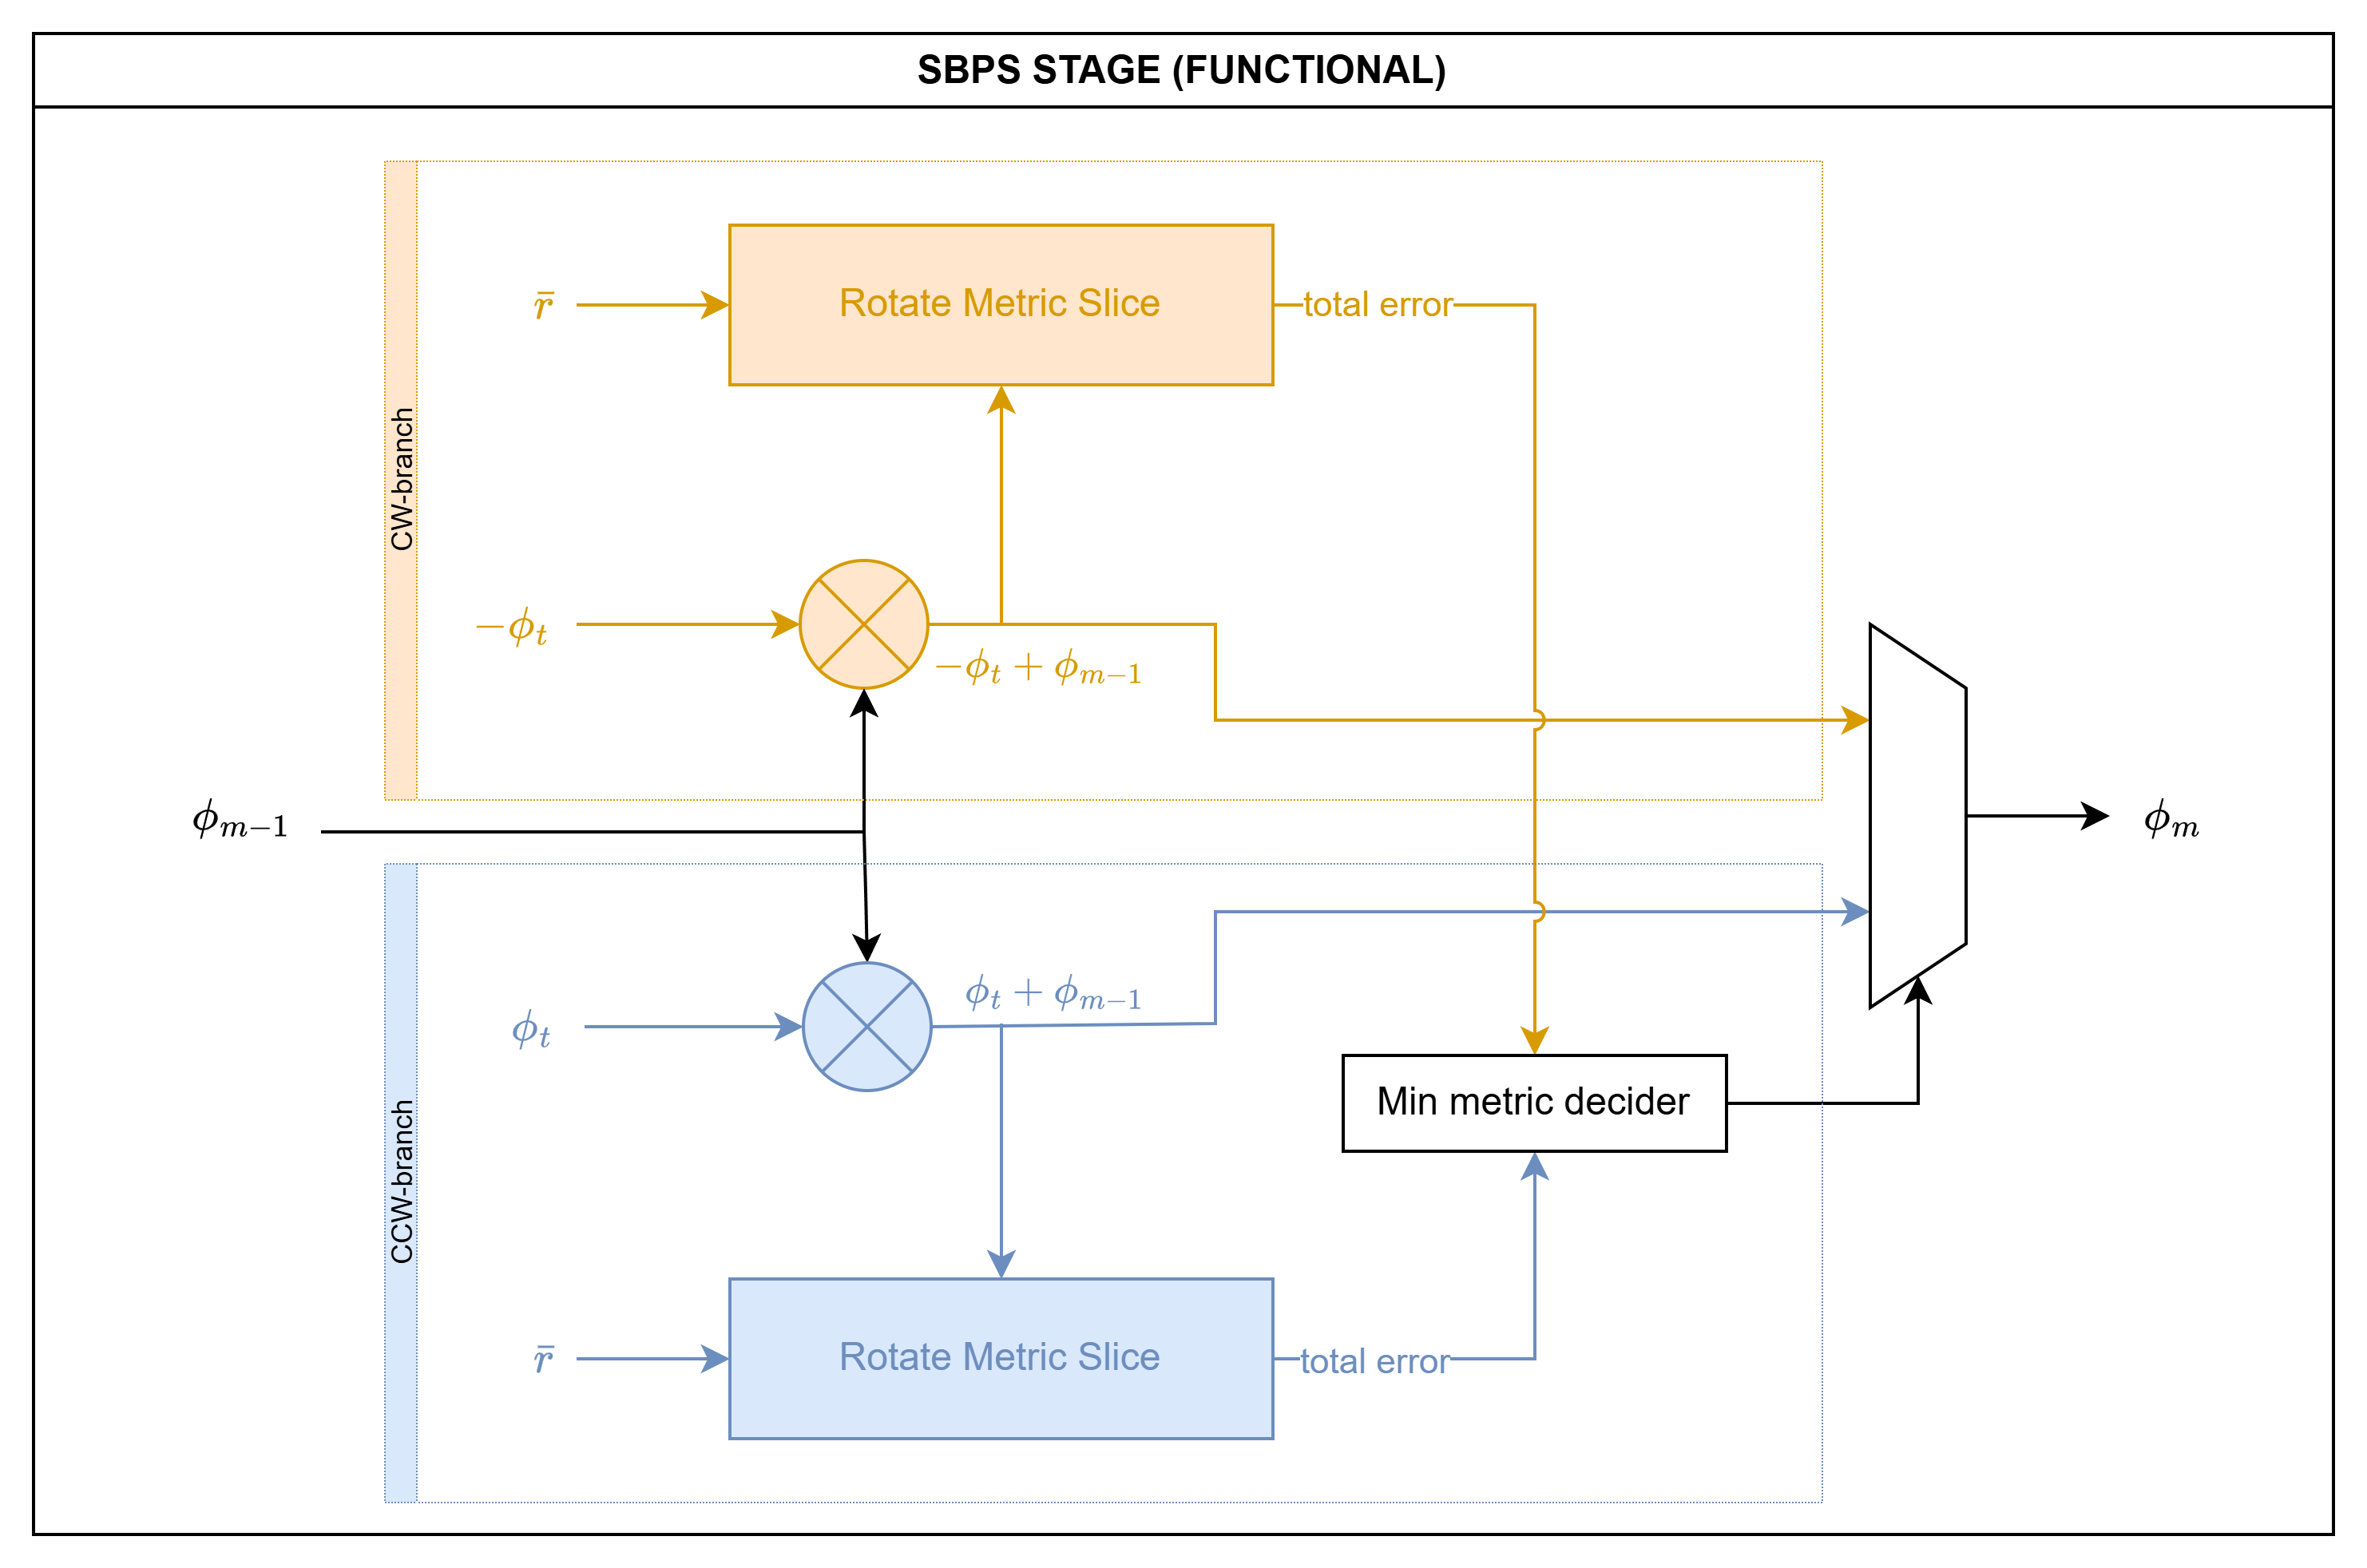
\includegraphics[width=1\linewidth]{figures/SBPS_stage_functional.png}
% \caption{Functional diagram of the SBPS stage}
% \label{fig:functional-SBPS-stage}
% \end{figure}




% The errors generated by both branches get compared by the \textit{min metric decider}, which in turn 
% is the select for the \ac{MUX} which lets only the correct guess through to the next stage in the pipeline.
% \\\\
% To go from block and test-angle to the error of that block, a functional block \textit{rotate metric slice} is defined (see figure \ref{fig:functional-rotate-slice-metric}).

% \begin{figure}[H]
% \centering
% 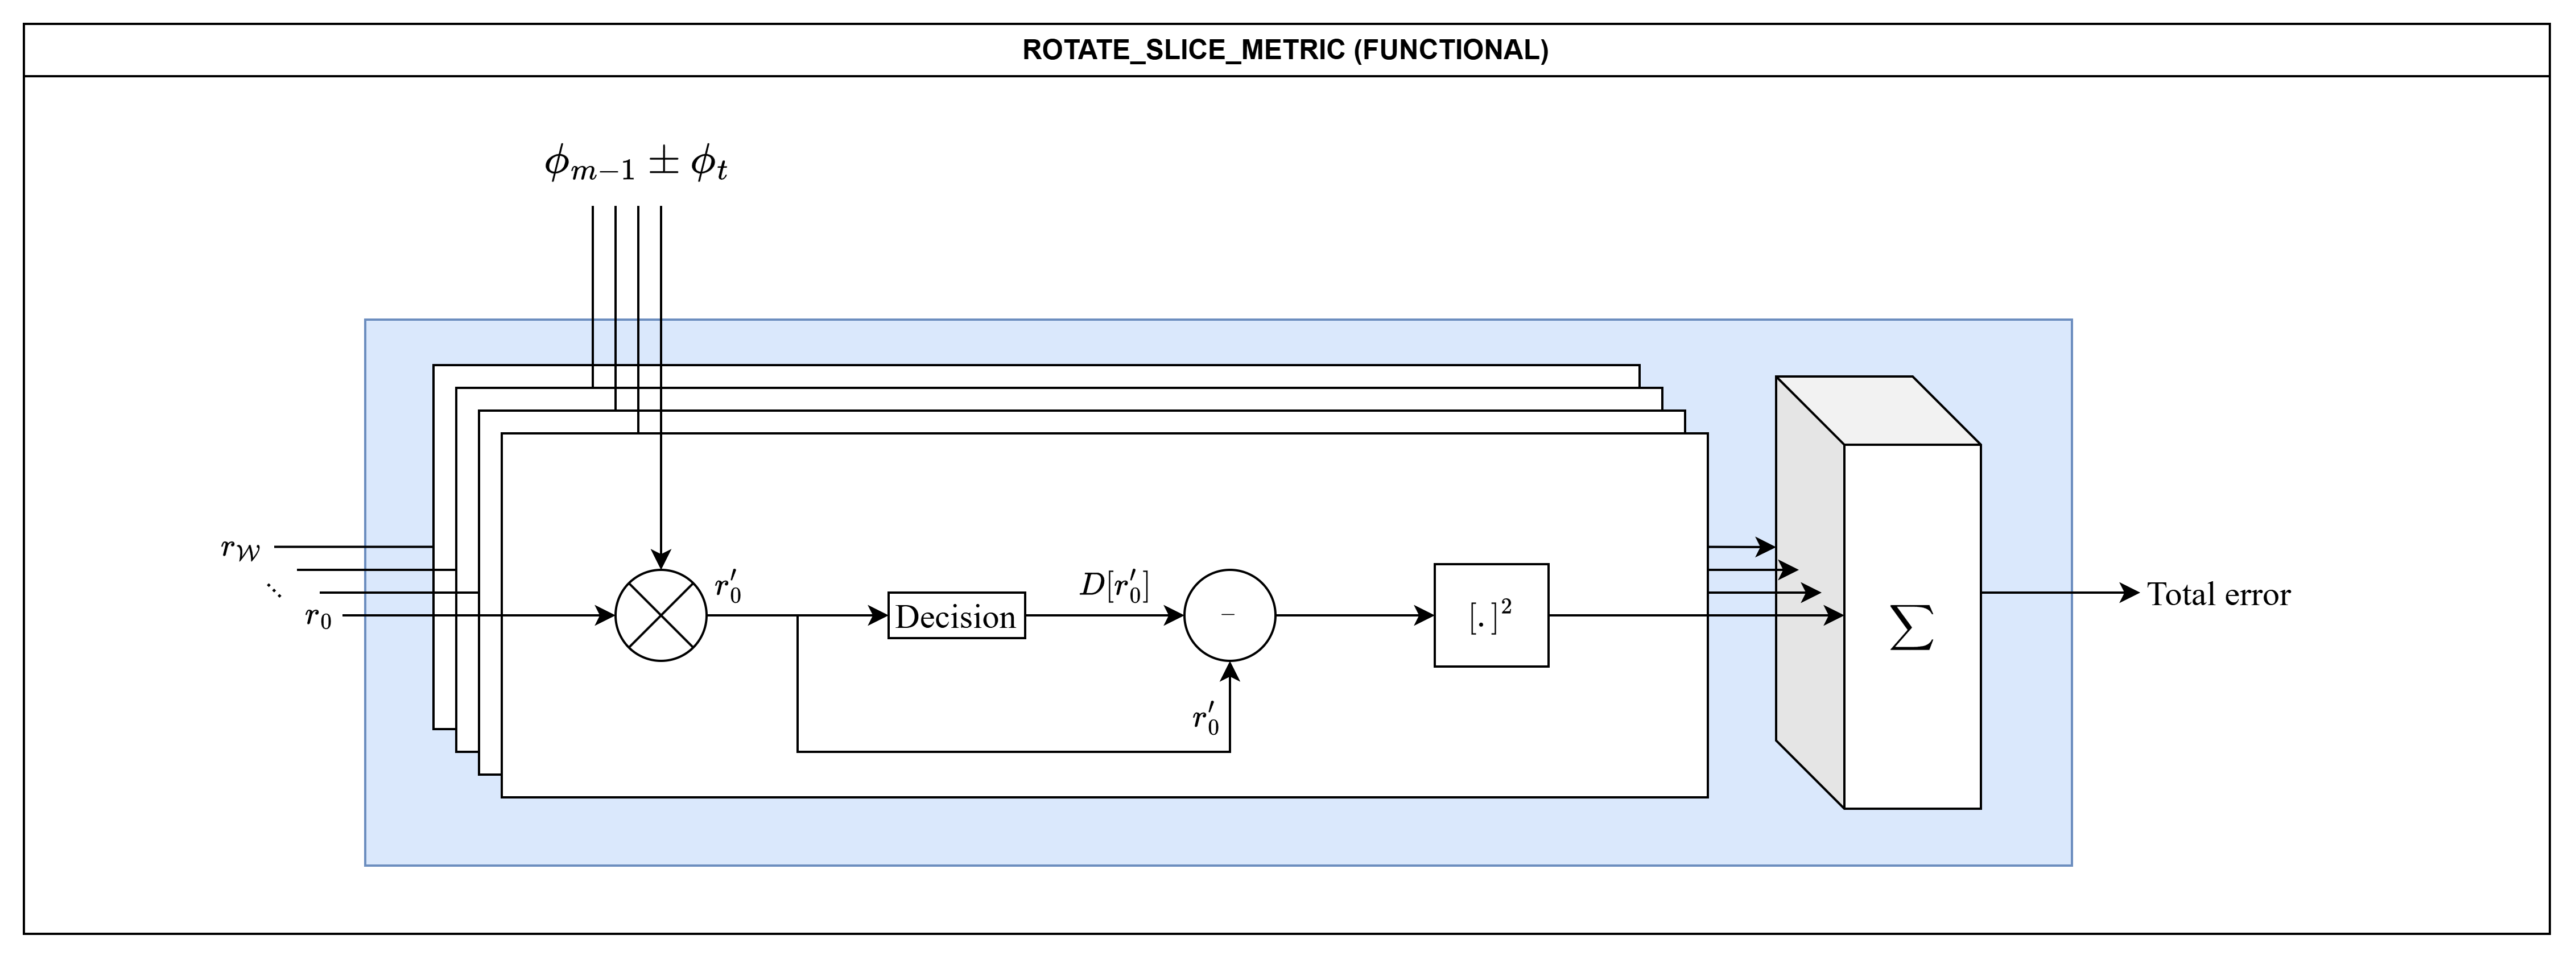
\includegraphics[width=1\linewidth]{figures/rotate_slice_metric_functional.png}
% \caption{Functional diagram of the rotate metric slice module}
% \label{fig:functional-rotate-slice-metric}
% \end{figure}

% The error of each symbol within the block is calculated in parallel, after which they get added to form the total error of the block.
% First, the symbols $ r $ are rotated by either $ e^{-j(\phi_t - \phi_{m-1})} $ for the counter-clockwise branch, or $ e^{-j(-\phi_t - \phi_{m-1})} $ for the clockwise branch.
% Second, these rotated symbols $ r' $ are sliced to the nearest 16QAM constallation point \footnote{exceptions apply for radius directed stages, wich will be covered in the next subsection}.
% These sliced symbols are denoted by $ D[r'] $, and the distance of these from the purely sliced symbols $ r' $ , squared, represent the error. 

% \subsubsection{Data-flow}
% Since the representation of certain inputs are non-trivial, it is worth exploring what is actually calculated to represent these values.
% \todo{insert section about SBPS data representation}


% \begin{figure}[h]
% \centering
% 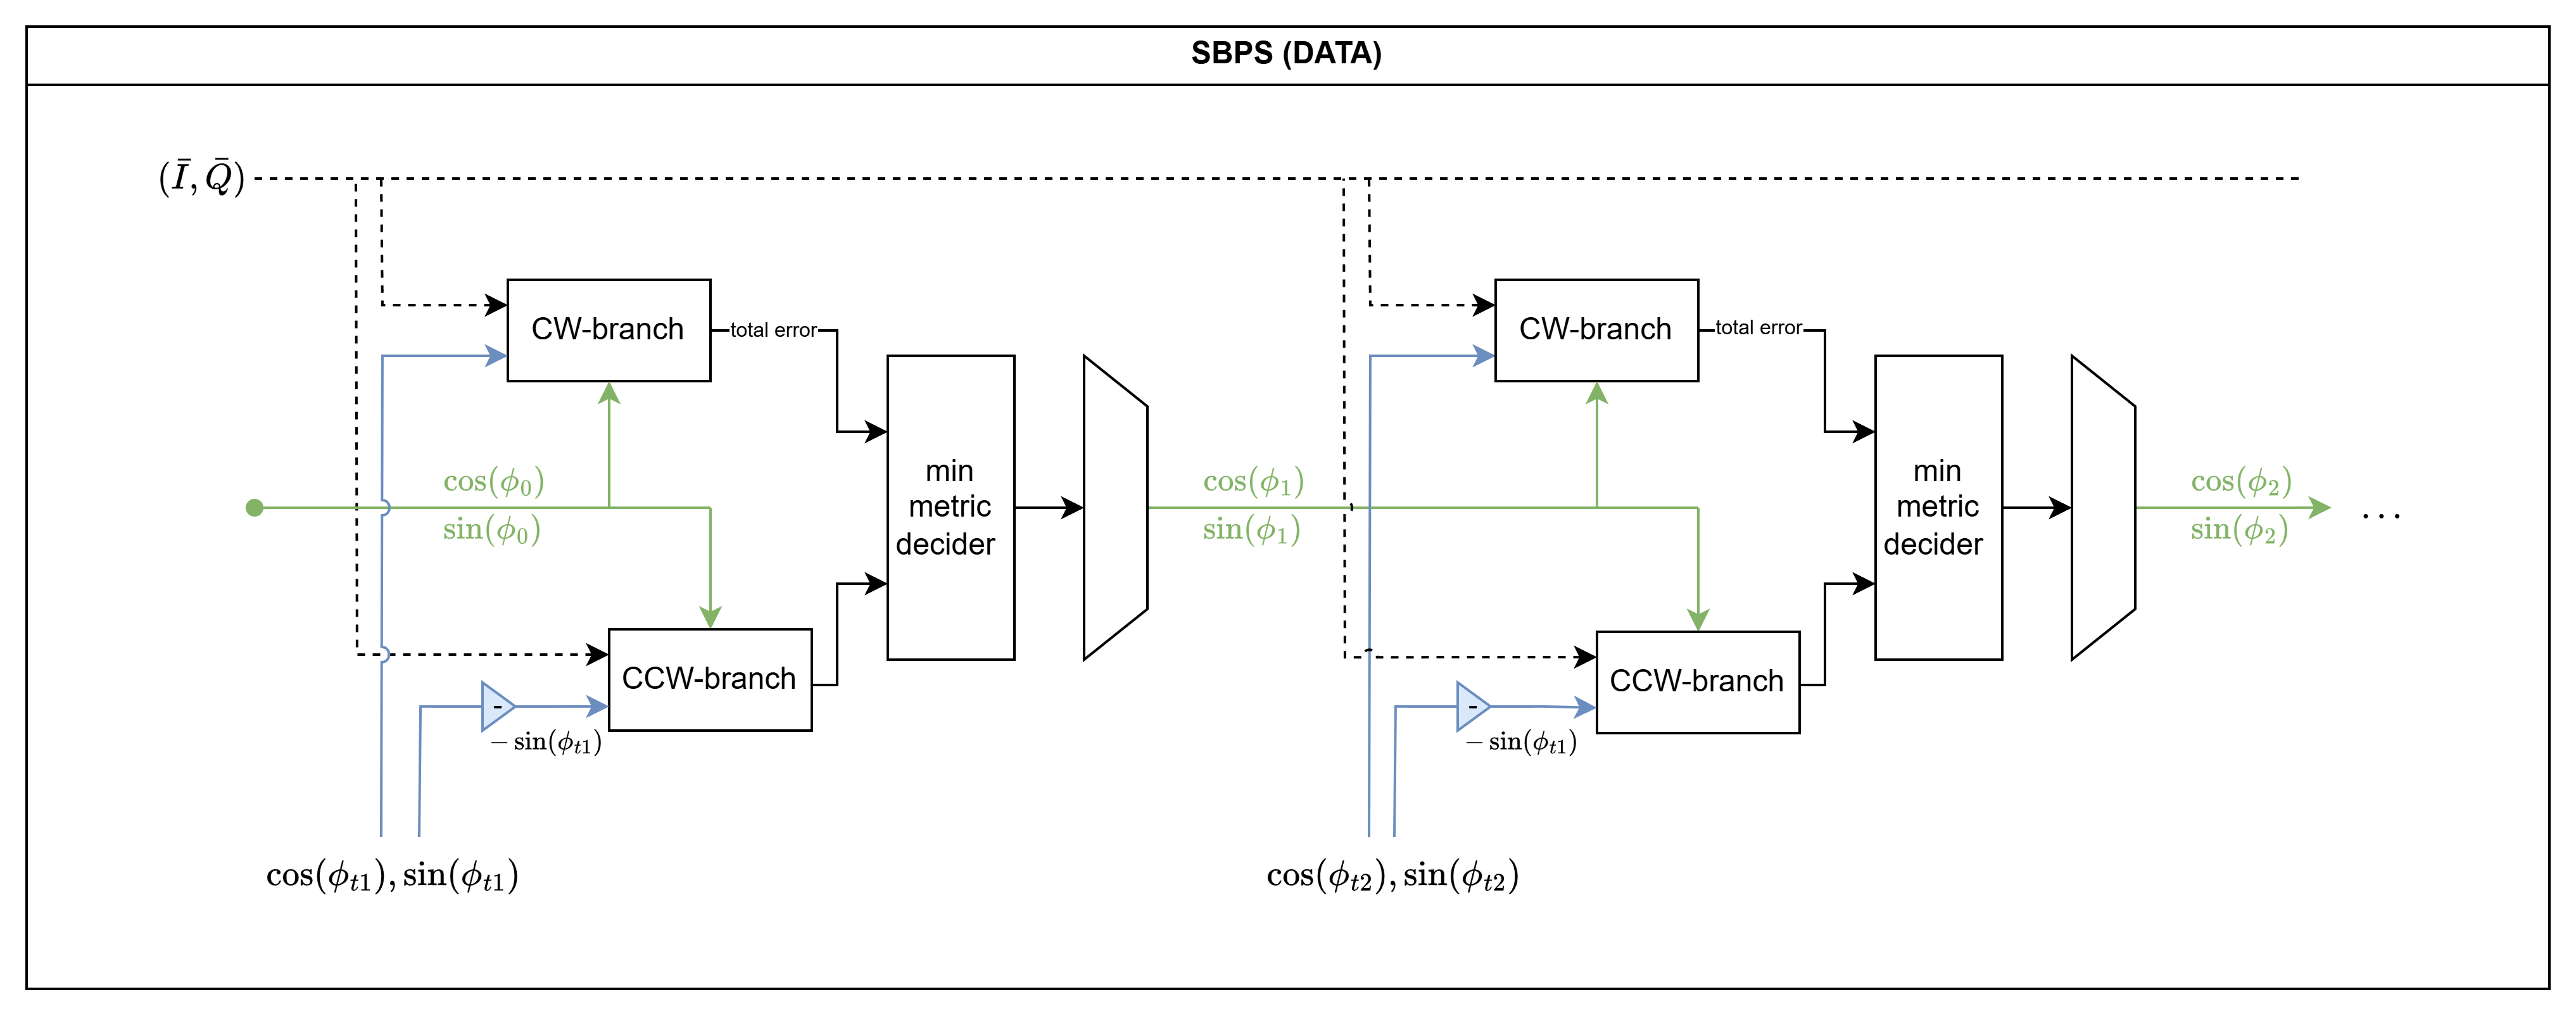
\includegraphics[width=1\linewidth]{figures/SBPS_data.png}
% \caption{Data-representative diagram of the rotate metric slice module}
% \label{fig:data-SBPS-full}
% \end{figure}


% \begin{figure}[h]
% \centering
% 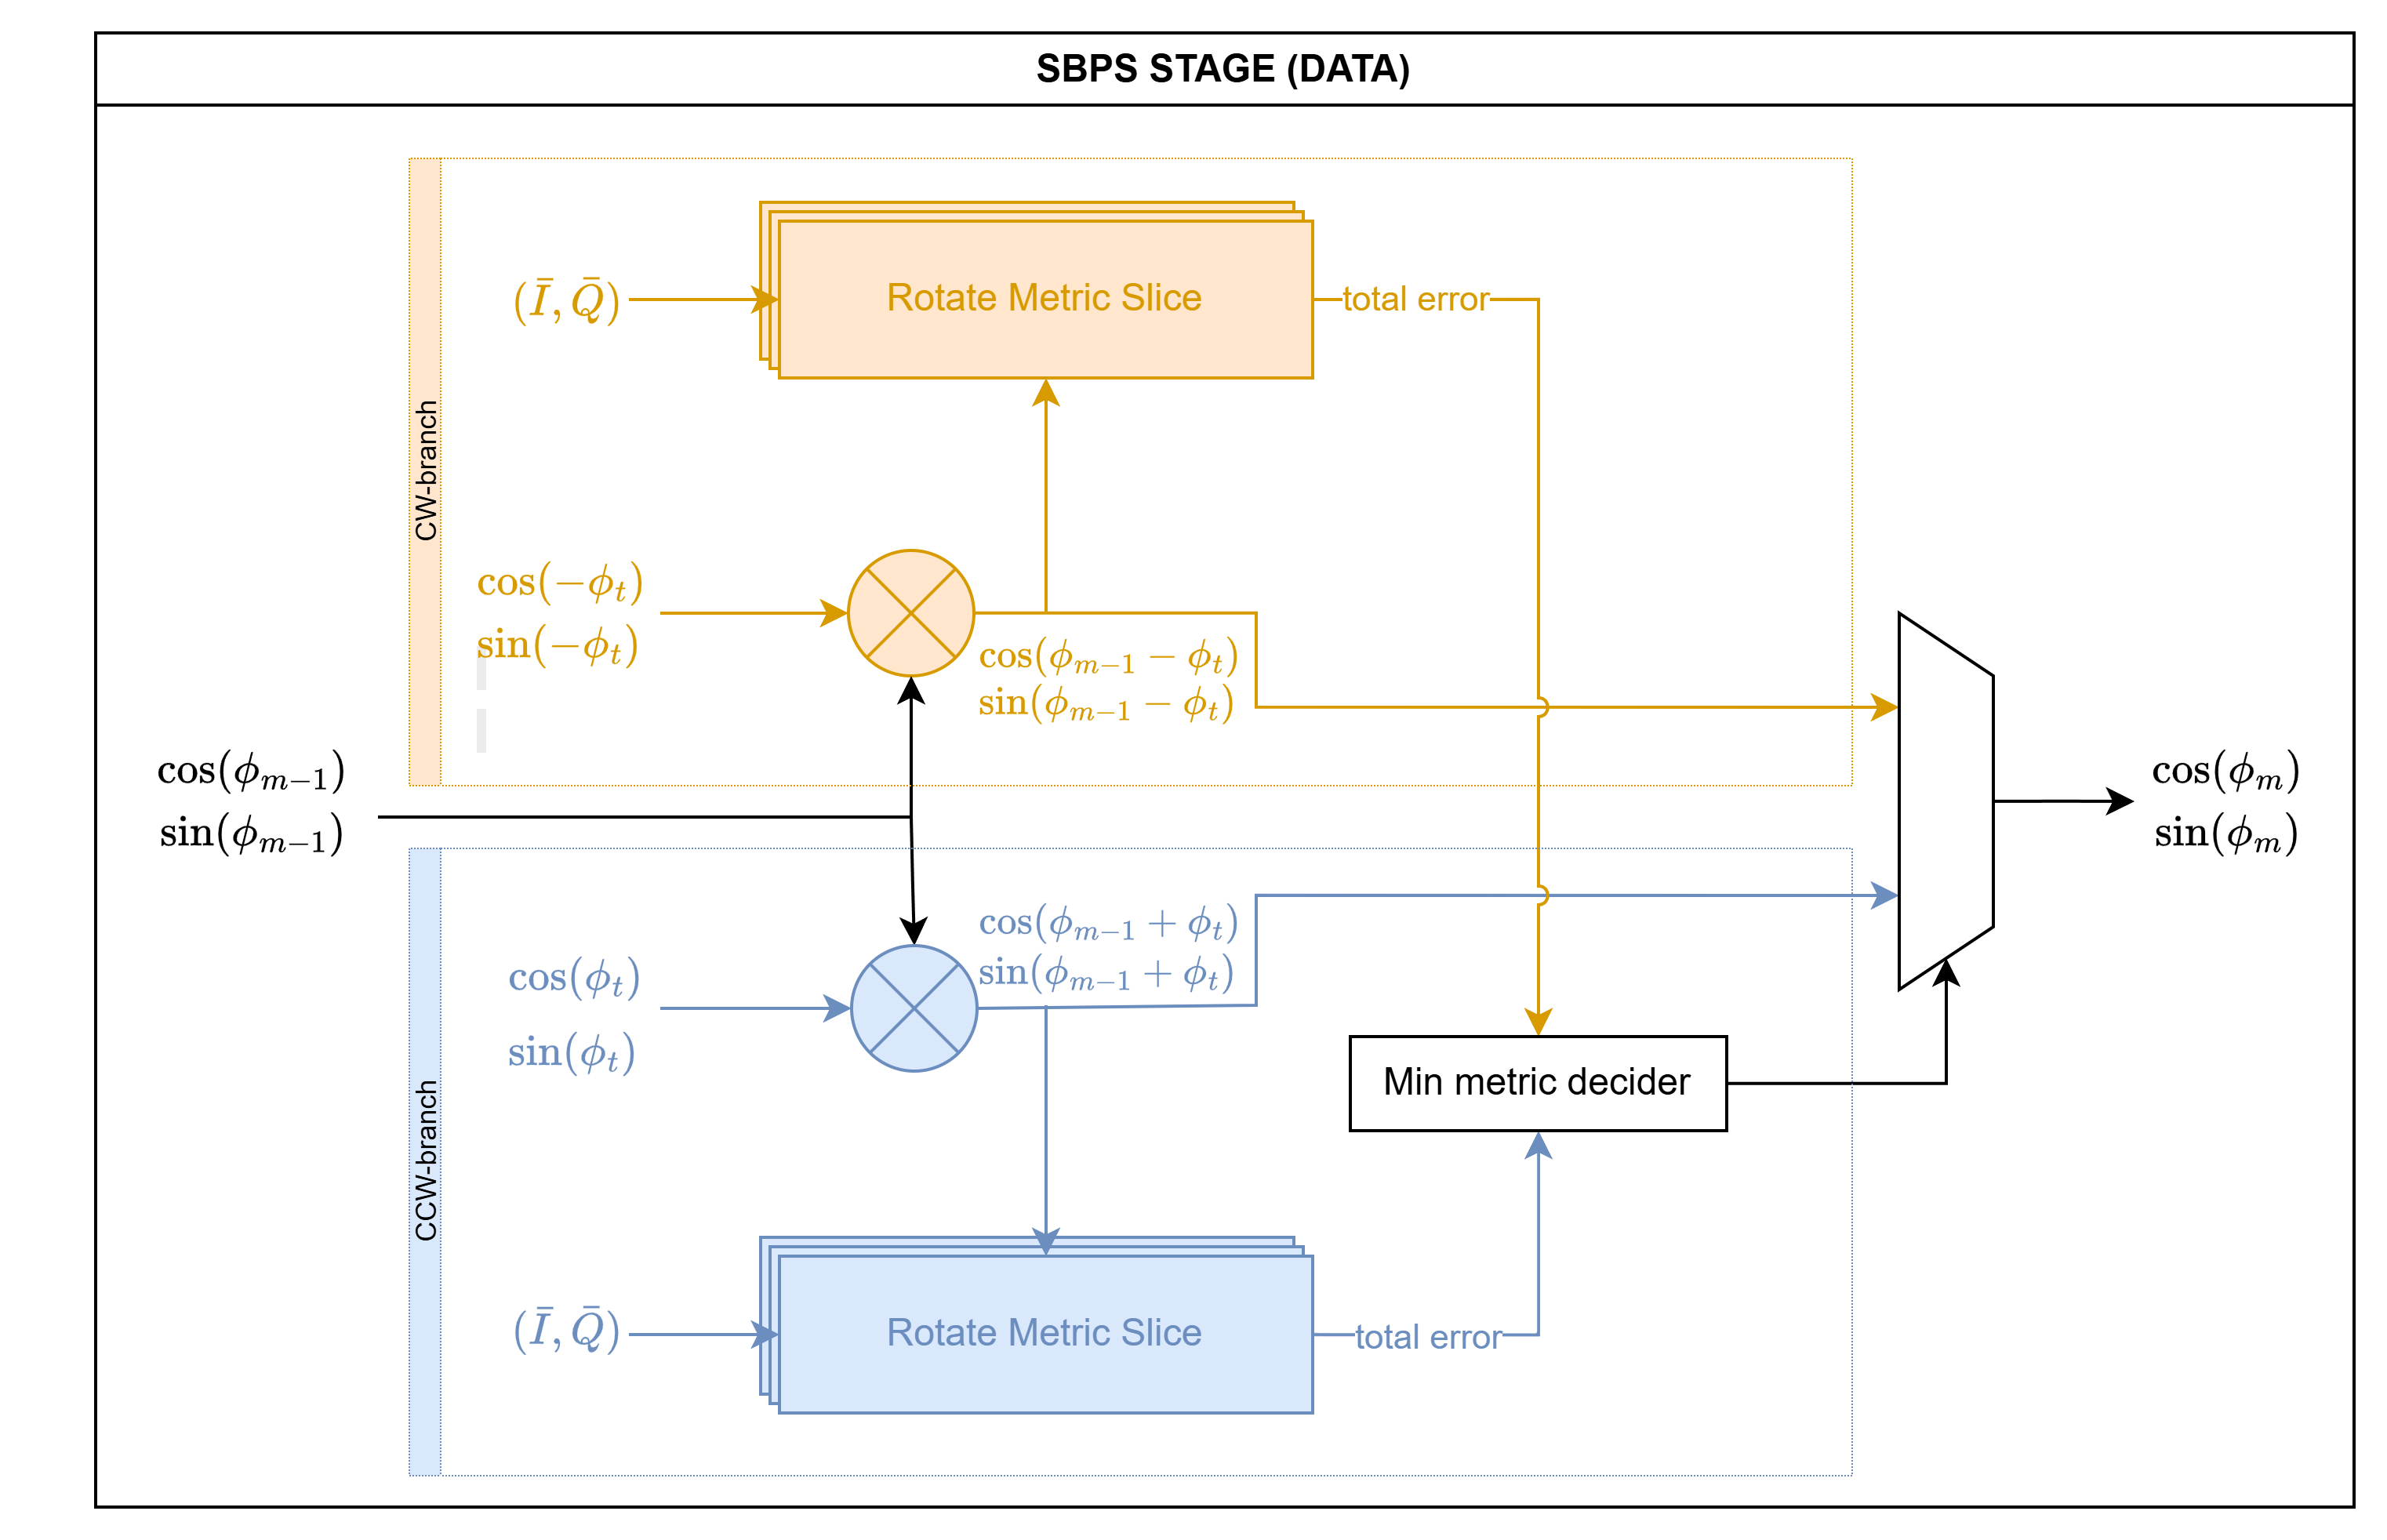
\includegraphics[width=1\linewidth]{figures/SBPS_stage_data.png}
% \caption{Data-representative diagram of the rotate metric slice module}
% \label{fig:data-SBPS-stage}
% \end{figure}

% \begin{figure}[h]
% \centering
% 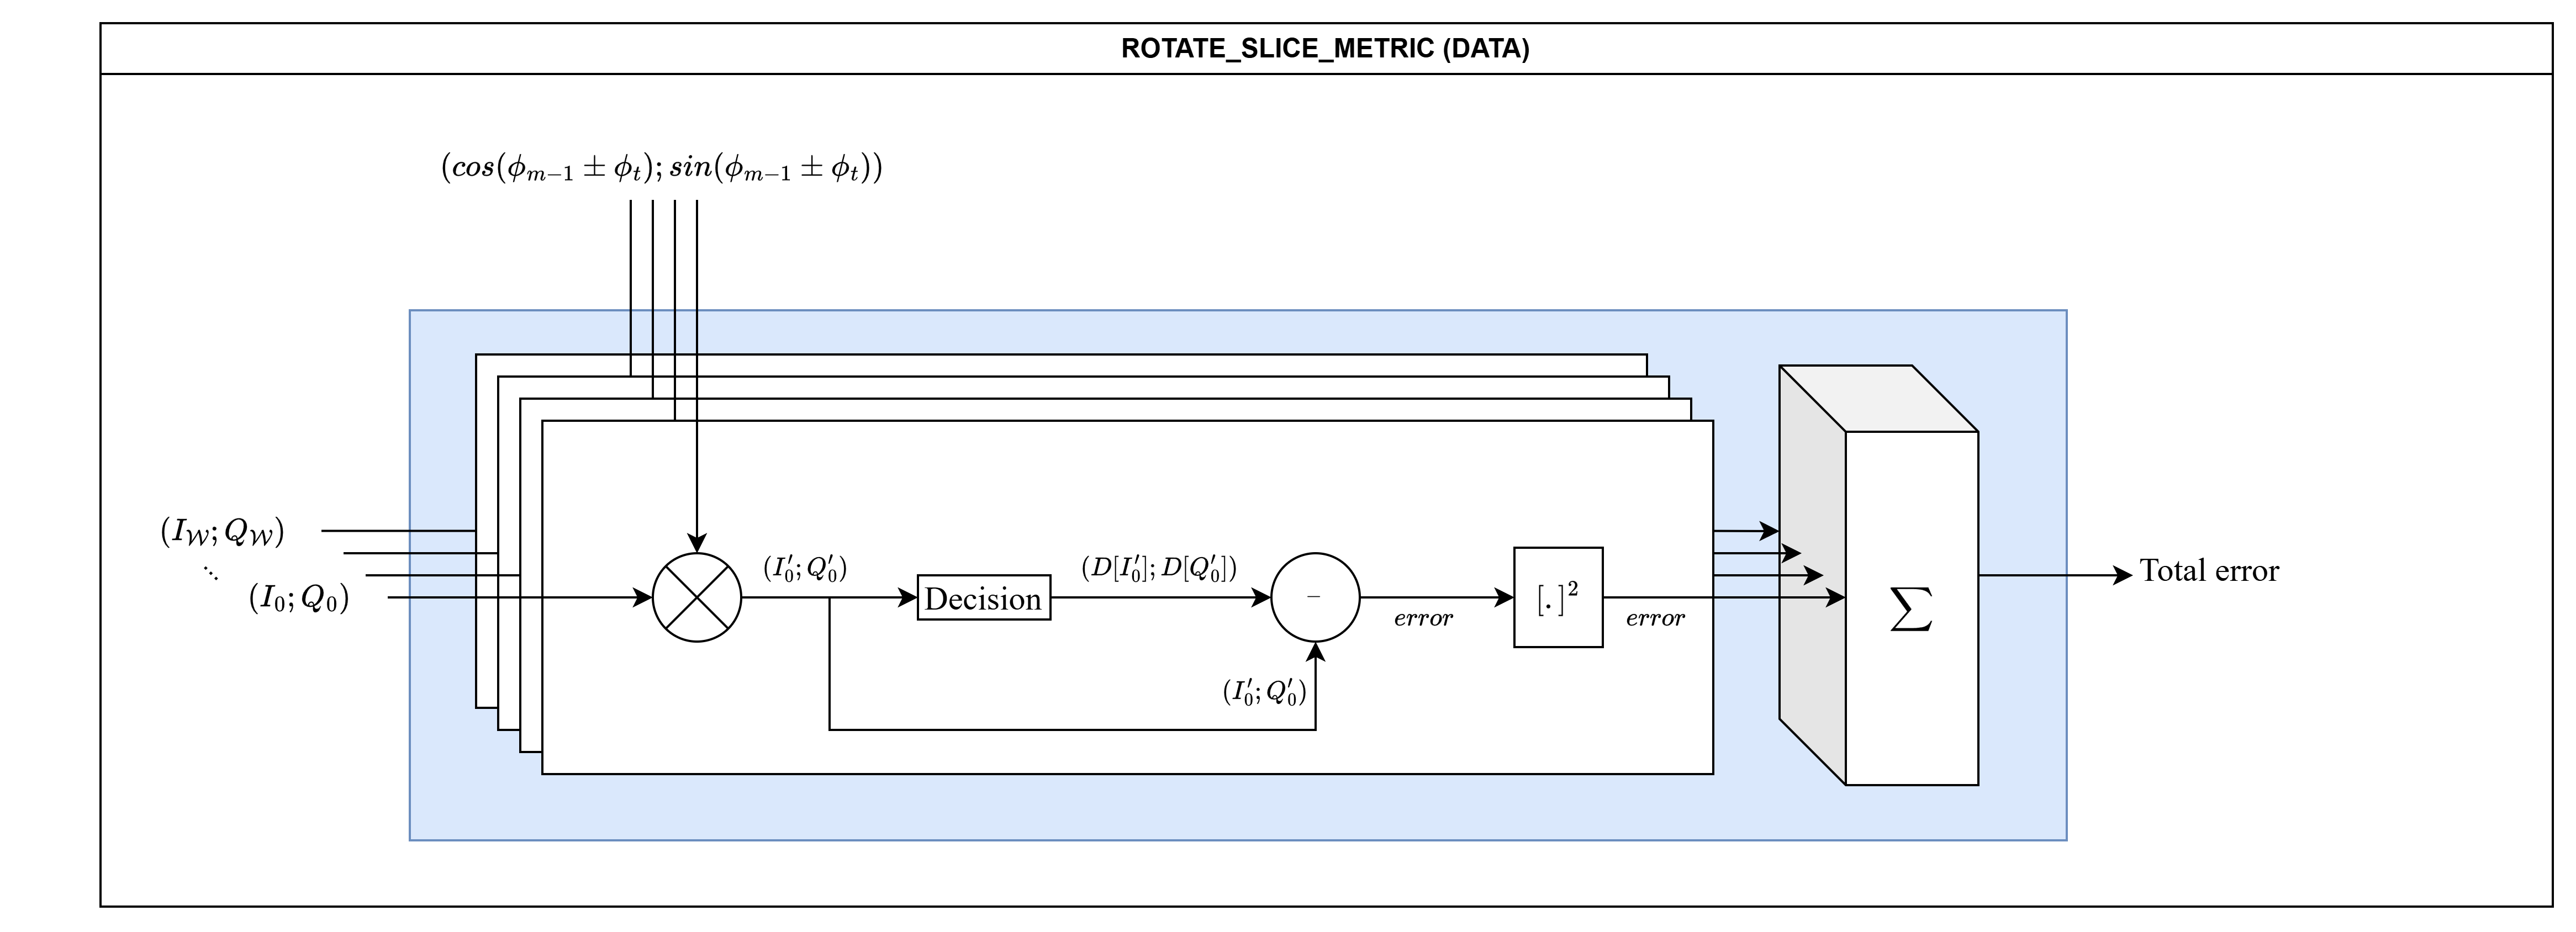
\includegraphics[width=1\linewidth]{figures/rotate_slice_metric_data.png}
% \caption{Data-representative diagram of the rotate metric slice module}
% \label{fig:data-rotate-slice-metric}
% \end{figure}

% Before the true test-angles $ \phi_{m-1} \pm \phi_t $ can be fed into the input of the \textit{rotate metric slice} block, they need to be calculated. 
% The summation of these angles are done in trigonometric form of $ ((cos(x); sin(x)) $, where $x$ is a fixed-point value. 
% The \textit{angle add} block does the following to represent the true test-angles in trigonometric form:

% $$ \cos(\phi_{m-1} \pm \phi_t) = \cos(\phi_{m-1})\cos(\phi_t) \mp \sin(\phi_{m-1})\sin(\phi_{t}) $$
% $$ \sin(\phi_{m-1} \pm \phi_t) = \sin(\phi_{m-1})\cos(\phi_{t}) \pm \cos(\phi_{m-1})\sin(\phi_{t}) $$

% Now, in order to effectively rotate the input samples - which are represented in $I/Q$-values - the following calculations are done on FPGA:
% \begin{equation} \label{eq:rotated_samples}
% \begin{aligned}
% I' &= I \cos(\phi_{m-1} \pm \phi_t) + Q \sin(\phi_{m-1} \pm \phi_t) \\
% Q' &= -I \sin(\phi_{m-1} \pm \phi_t) + Q \cos(\phi_{m-1} \pm \phi_t)
% \end{aligned}
% \end{equation}


% Next, the decision-making rests on comparators and certain pre-calculated values for the constellation-threshold $\pm 2s$. \todo{maybe explain clearer?, maybe already done in section 3?}

% \begin{equation} \label{eq:slice_function}
% \begin{aligned}
% &|I'| \leq 2s ,
% &|Q'| \leq 2s 
% \end{aligned}
% \end{equation}

% Then, a subtraction of the rotated and sliced symbols $ D[I', Q'] $ is done from rotated symbols $ (I', Q') $. 
% Finally, 2 products are performed to calculate the squared values of that difference in I and Q terms.

% \todo{insert equation that represent the data-path calculation for the single symbol squared error} \label{eq:single-symbol-error} 

% This step also includes optional resizing of the output, since the output error is a parameter in the design block. 
% \\\\

% Finally, this single-symbol squared error gets accumulated for each symbol over the block window $ \cal W $.
% \subsubsection{Timing-flow}

% The \textit{angle add} module that calculates each stage's true test-angles $ \phi_{m-1} \pm \phi_t $ has 3 clockcycles of latency. The first clockcycle calculates the trigonometric
% multiplications, the second does sum/difference and shift, and finally a final saturating output register.

% The block samples $ \bar r $ need to be synchronously fed into the \textit{rotate metric slice} module, so these also get 
% delayed by 3 clockcycles, matching the \textit{angle add} module.

% \begin{figure}[h]
% \centering
% 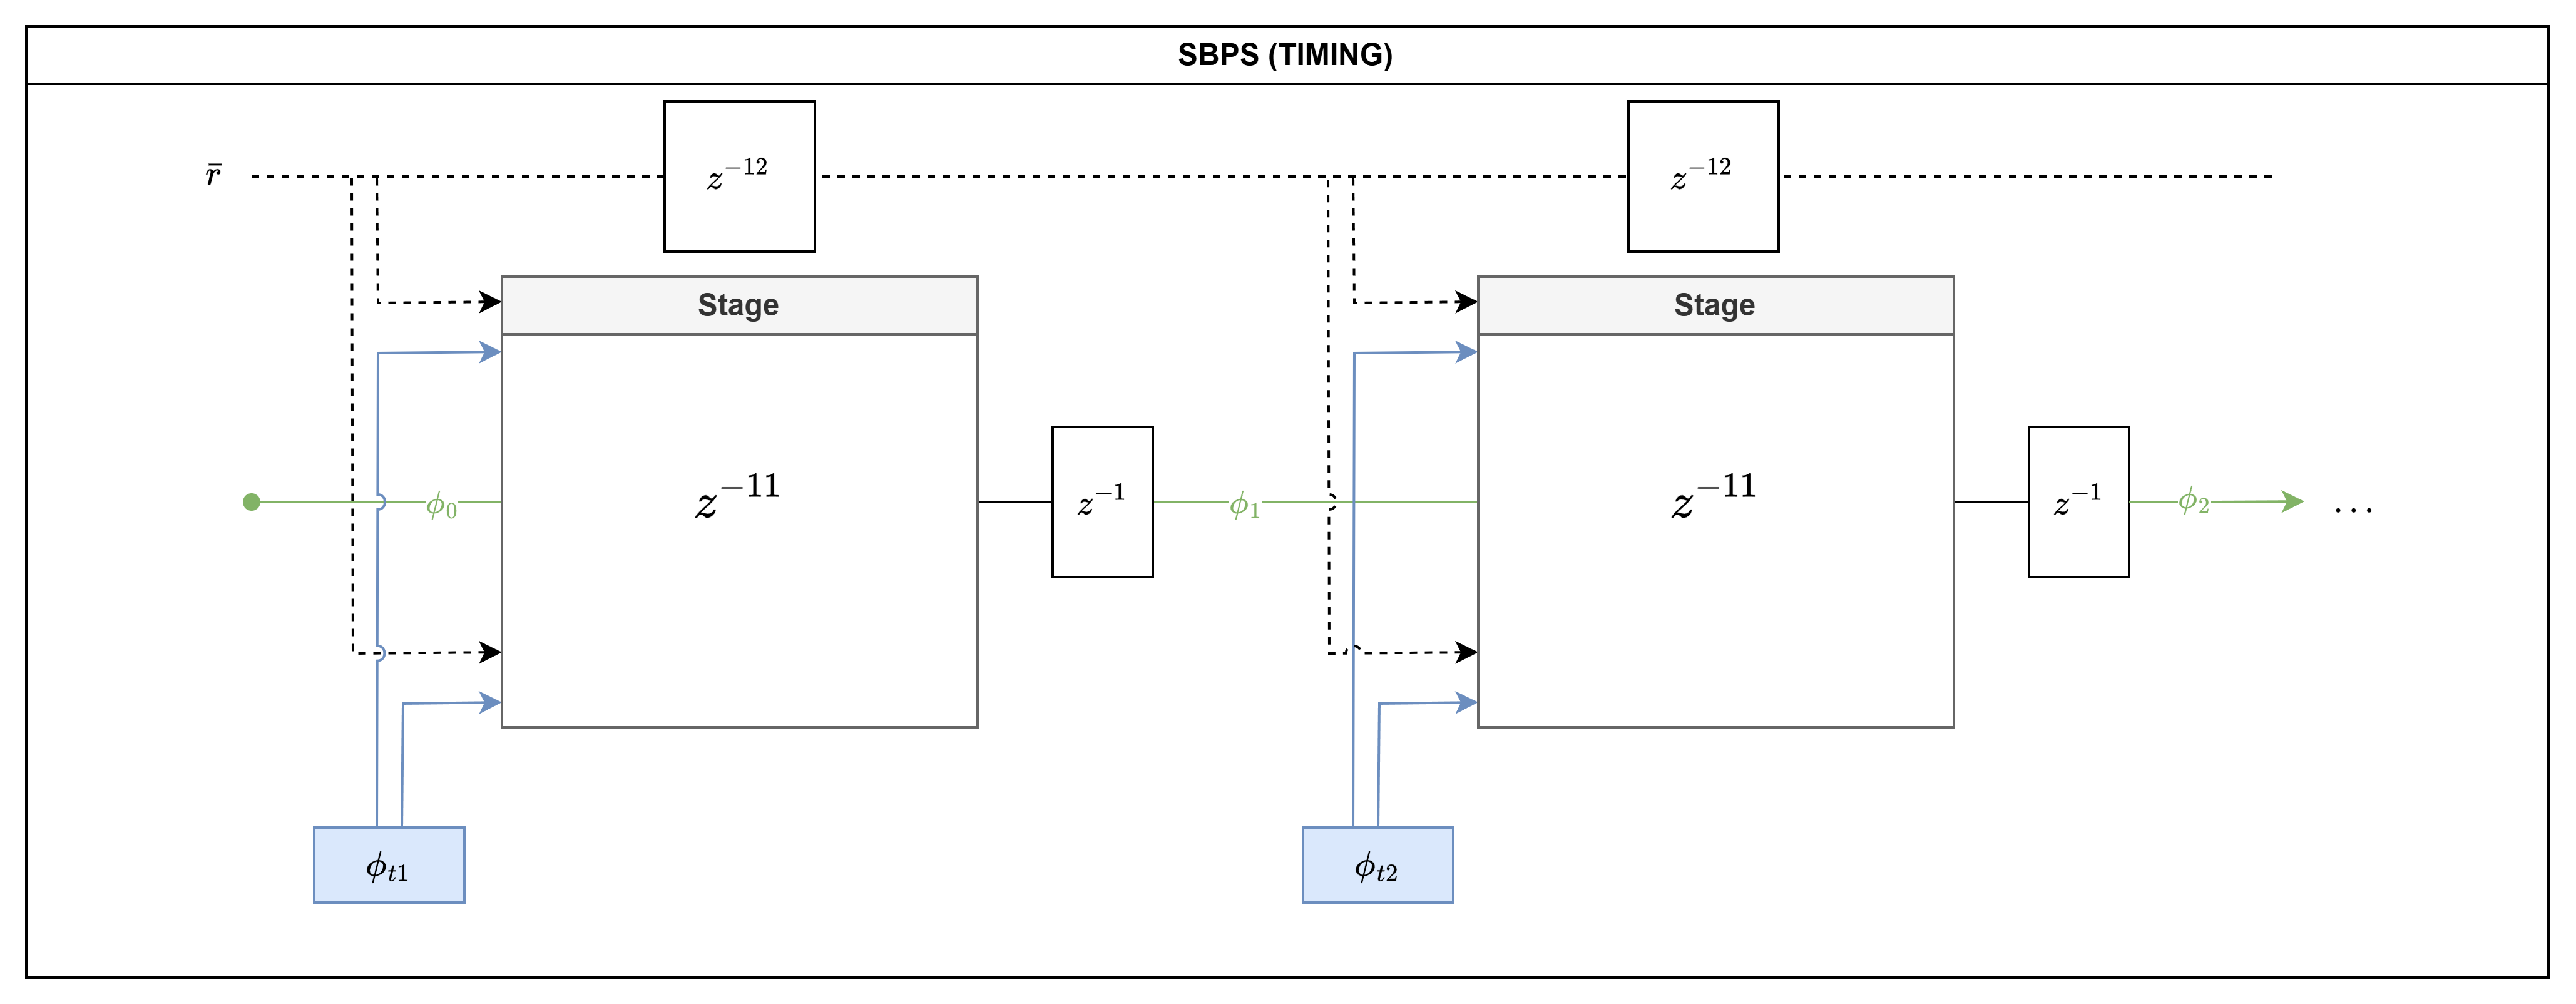
\includegraphics[width=1\linewidth]{figures/SBPS_timing.png}
% \caption{Timing diagram of the full SBPS module}
% \label{fig:timing-SBPS-full}
% \end{figure}

% \begin{figure}[h]
% \centering
% 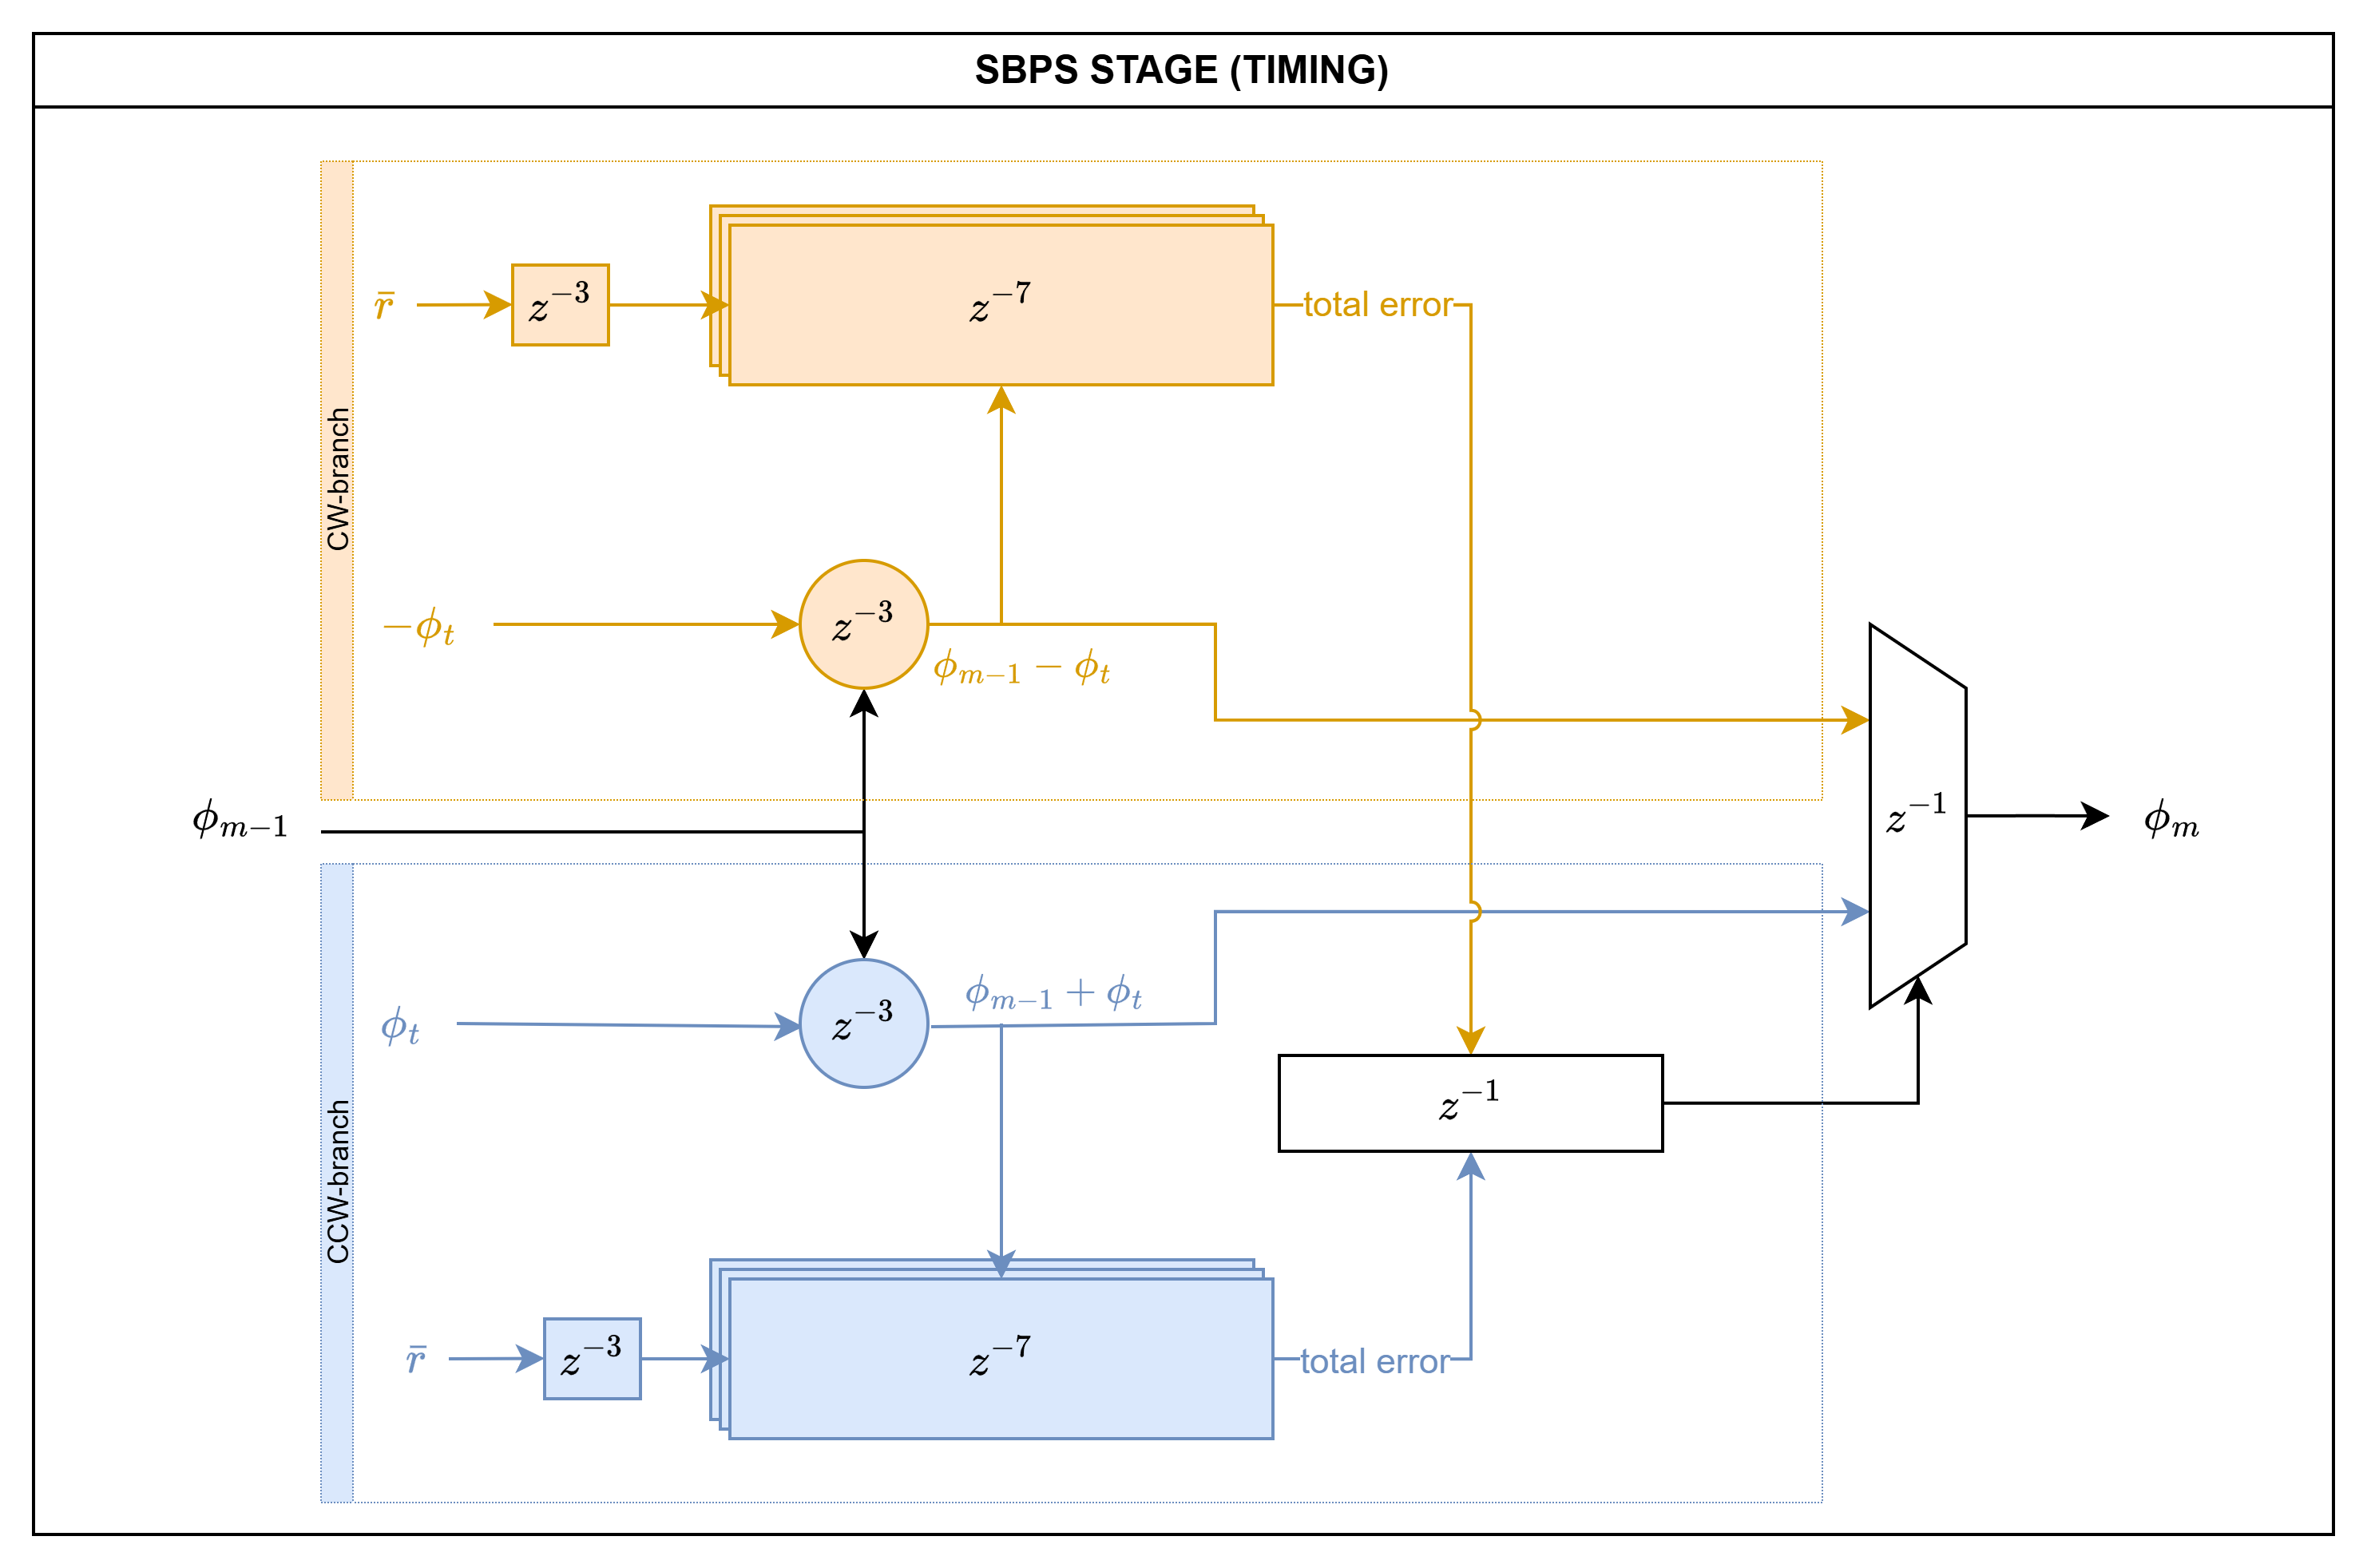
\includegraphics[width=1.1\linewidth]{figures/SBPS_stage_timing.png}
% \caption{Timing diagram of the SBPS stage design}
% \label{fig:timing-SBPS-stage}
% \end{figure}

% After each branch has calculated the total error after 7 clockcycles (see next paragraph), the \textit{
% min metric decider} module takes 1 cycle to select the minimum error and feeding it to the \ac{MUX}. 
% The MUX then outputs the relevent $ \phi_m $ as either $ \phi_{m-1} \pm \phi_t $ according to which one has
% the smallest accumulated error. 
% \\\\
% The 7 cycle delay from the \textit{rotate metric slice} module is shown in more detail on figure \ref{fig:timing_rotate_metric_slice}.
% Rotating the incoming symbols $ \bar r $ takes 3 cycles. 
% The three registered stages consist of first calculating the trigonometric multiplications of equation \ref{eq:rotated_samples}.
% Second, these multiplications get added/subtracted and shifted for appropriate bitlengths (as the trigonometric resolution
% is also a parameter in the RTL design). At last, saturation and the output registers are handled. 

% \begin{figure}[h]
% \centering
% 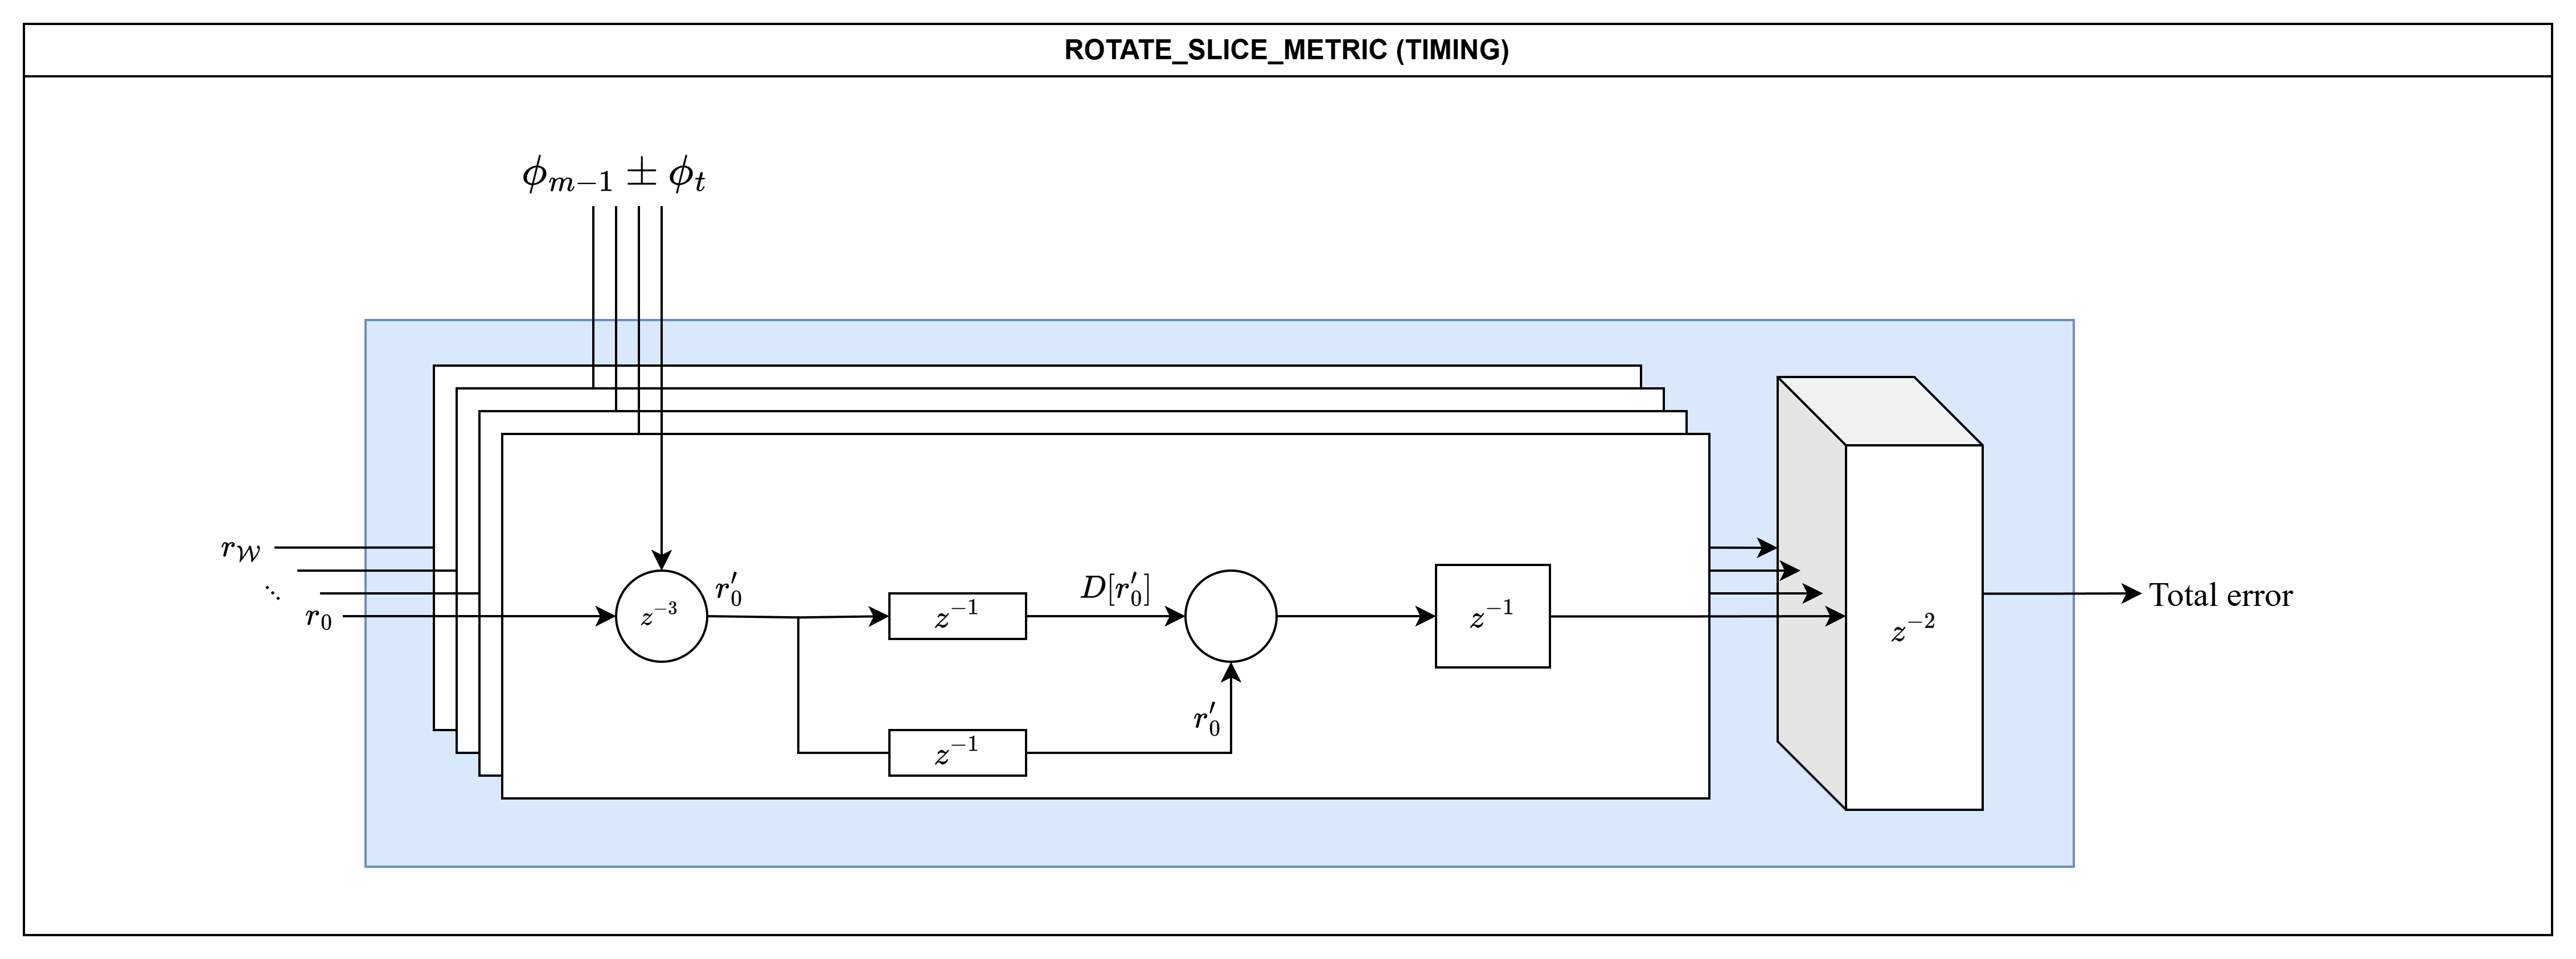
\includegraphics[width=1\linewidth]{figures/rotate_slice_metric_timing.png}
% \caption{Timing diagram of the rotate metric slice module}
% \label{fig:timing_rotate_metric_slice}
% \end{figure}

% After that, one registered process maps rotated I/Q to QPSK/16QAM reference symbols. Since these calculations are purely 
% comparative (equation \ref{eq:slice_function}).
% But, since these sliced symbols need to be synchronous with the non-sliced symbols for error calcution, the purely rotated samples are 
% also delayed 1 cycle. 



% The metric calculations shown in equation \ref{eq:single-symbol-error} are done in one registered stage,
% after which the per-lane errors are summed into the accumulated error (1 cycle), then assigned to the output
% on the next clock.  

% \subsubsection{16QAM-specific adaptations}
% explain here how radius directed decision is deployed in slicer using $ l $ as new threshhold. 




\section{Serialized blind phase search block}

The hardware implementation follows a staged refinement architecture, shown in Fig.~\ref{fig:functional-SBPS}. The same received block
\[
\bar r = \left(r_0, r_1, \ldots, r_{\mathcal W-1}\right)
\]
is presented to every stage, while only the accumulated phase estimate is updated from stage to stage. 
At stage \(m\), two candidate phase updates are evaluated around the previously selected estimate 
\(\phi_{m-1}\), namely \(\phi_{m-1}-\phi_t\) and \(\phi_{m-1}+\phi_t\). The candidate that produces 
the smaller block error is selected as the stage output \(\phi_m\), which is then forwarded to the next stage. 
By cascading several stages with progressively smaller test angles, the architecture converges towards the phase 
estimate associated with the centre of the block.

\begin{figure}[H]
\centering
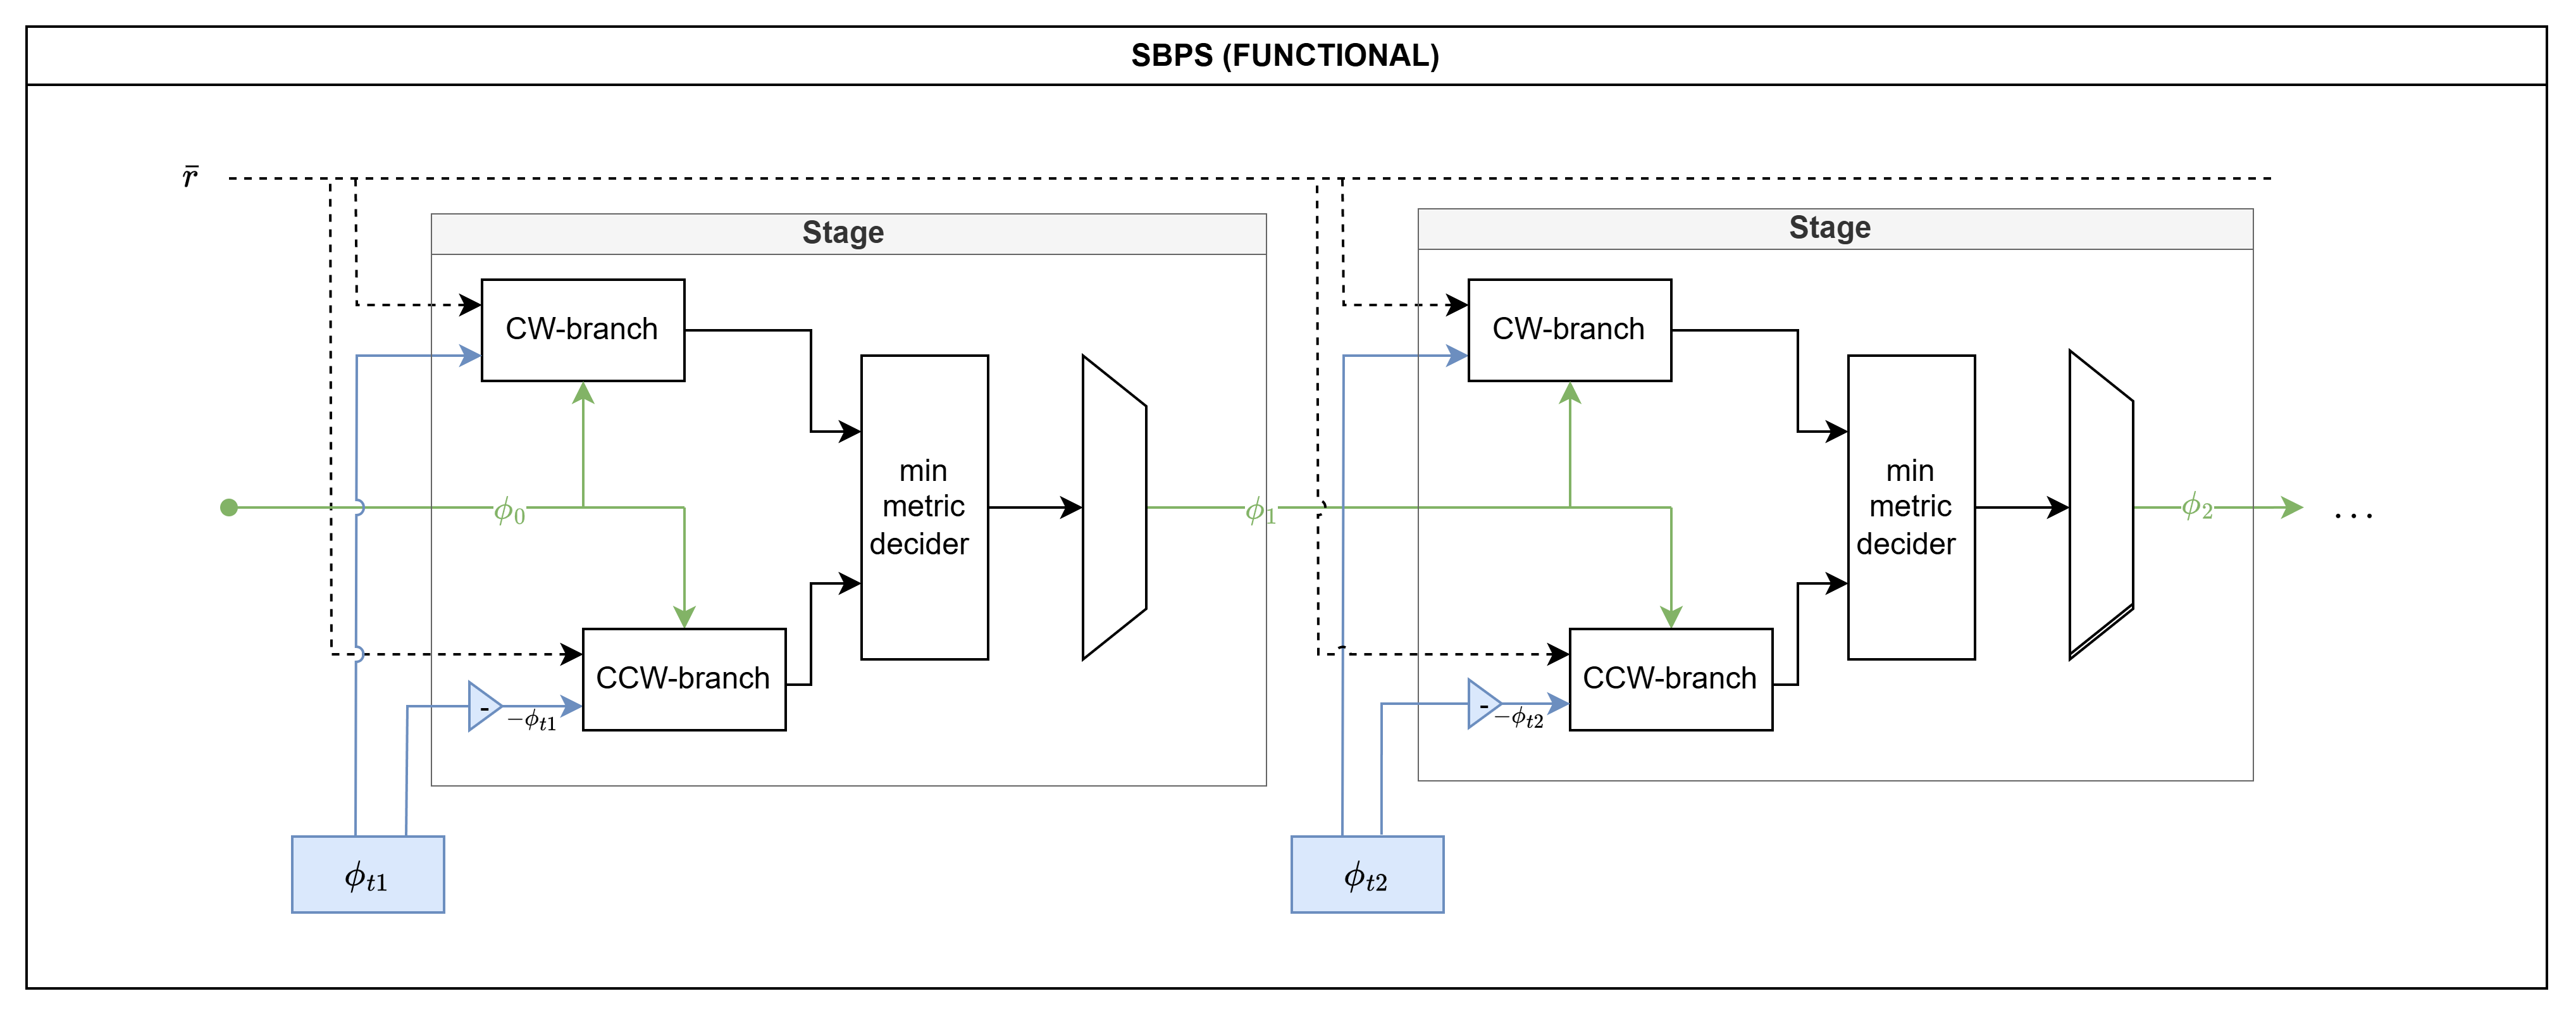
\includegraphics[width=1\linewidth]{figures/SBPS_functional.png}
\caption{Functional diagram of the full SBPS architecture }
\label{fig:functional-SBPS}
\end{figure}


\subsection{Functional operation}

Figure~\ref{fig:functional-SBPS-stage} shows the internal organisation of a single stage. The upper branch corresponds to the clockwise (CW) update and evaluates \(\phi_{m-1}-\phi_t\), whereas the lower branch corresponds to the counter-clockwise (CCW) update and evaluates \(\phi_{m-1}+\phi_t\). Each branch contains a \textit{rotate metric slice} unit that processes the complete input block using its own candidate phase. The resulting block metrics are compared by the \textit{min metric decider}, and the associated candidate phase is selected by the final \ac{MUX}. In this way, each stage performs a binary phase refinement around the current estimate.

\begin{figure}[H]
\centering
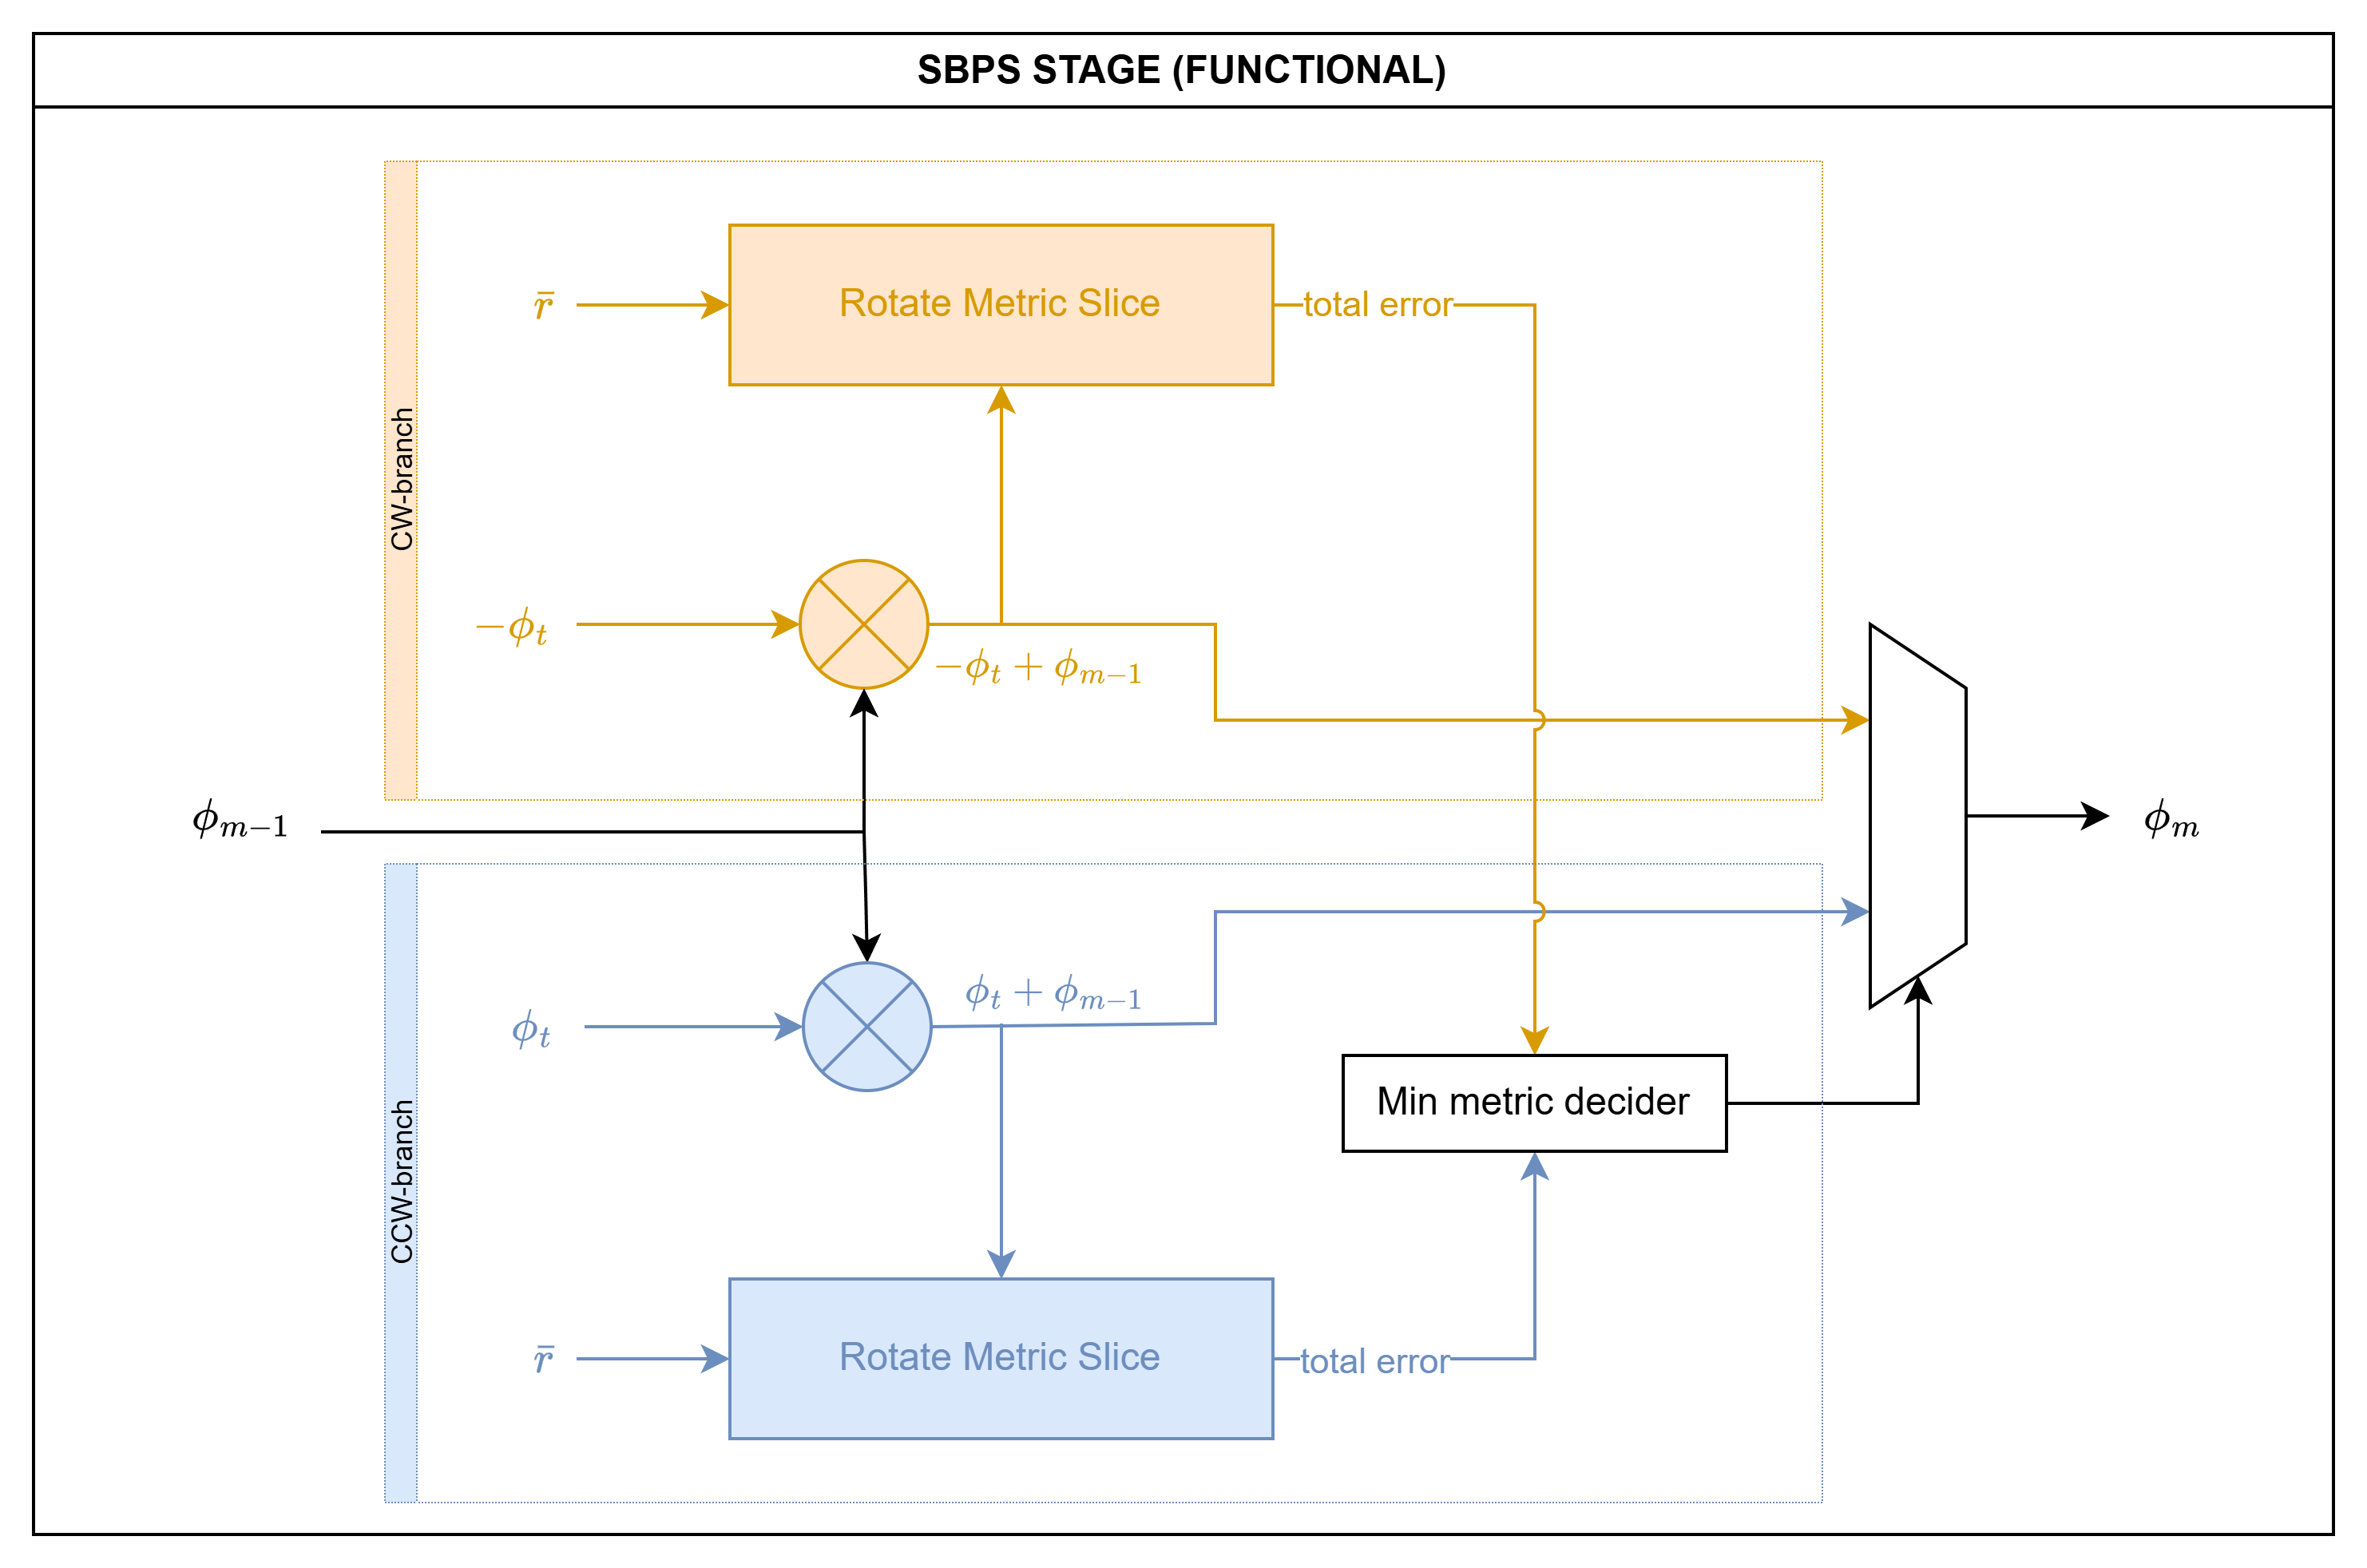
\includegraphics[width=0.8\linewidth]{figures/SBPS_stage_functional.png}
\caption{Functional diagram of the SBPS stage}
\label{fig:functional-SBPS-stage}
\end{figure}

The \textit{rotate metric slice} unit is the core computational block of the design and is detailed in Fig.~\ref{fig:functional-rotate-slice-metric}. For every symbol in the block, the candidate phase is used to rotate the received sample, the rotated sample is sliced to the nearest constellation point, and the squared Euclidean distance between the rotated and sliced values is computed. These per-symbol errors are then accumulated over the full block window to obtain a single decision metric for the branch. All symbols in the block are therefore processed in parallel inside each branch, while the serial refinement occurs across the SBPS stages.

\begin{figure}[H]
\centering
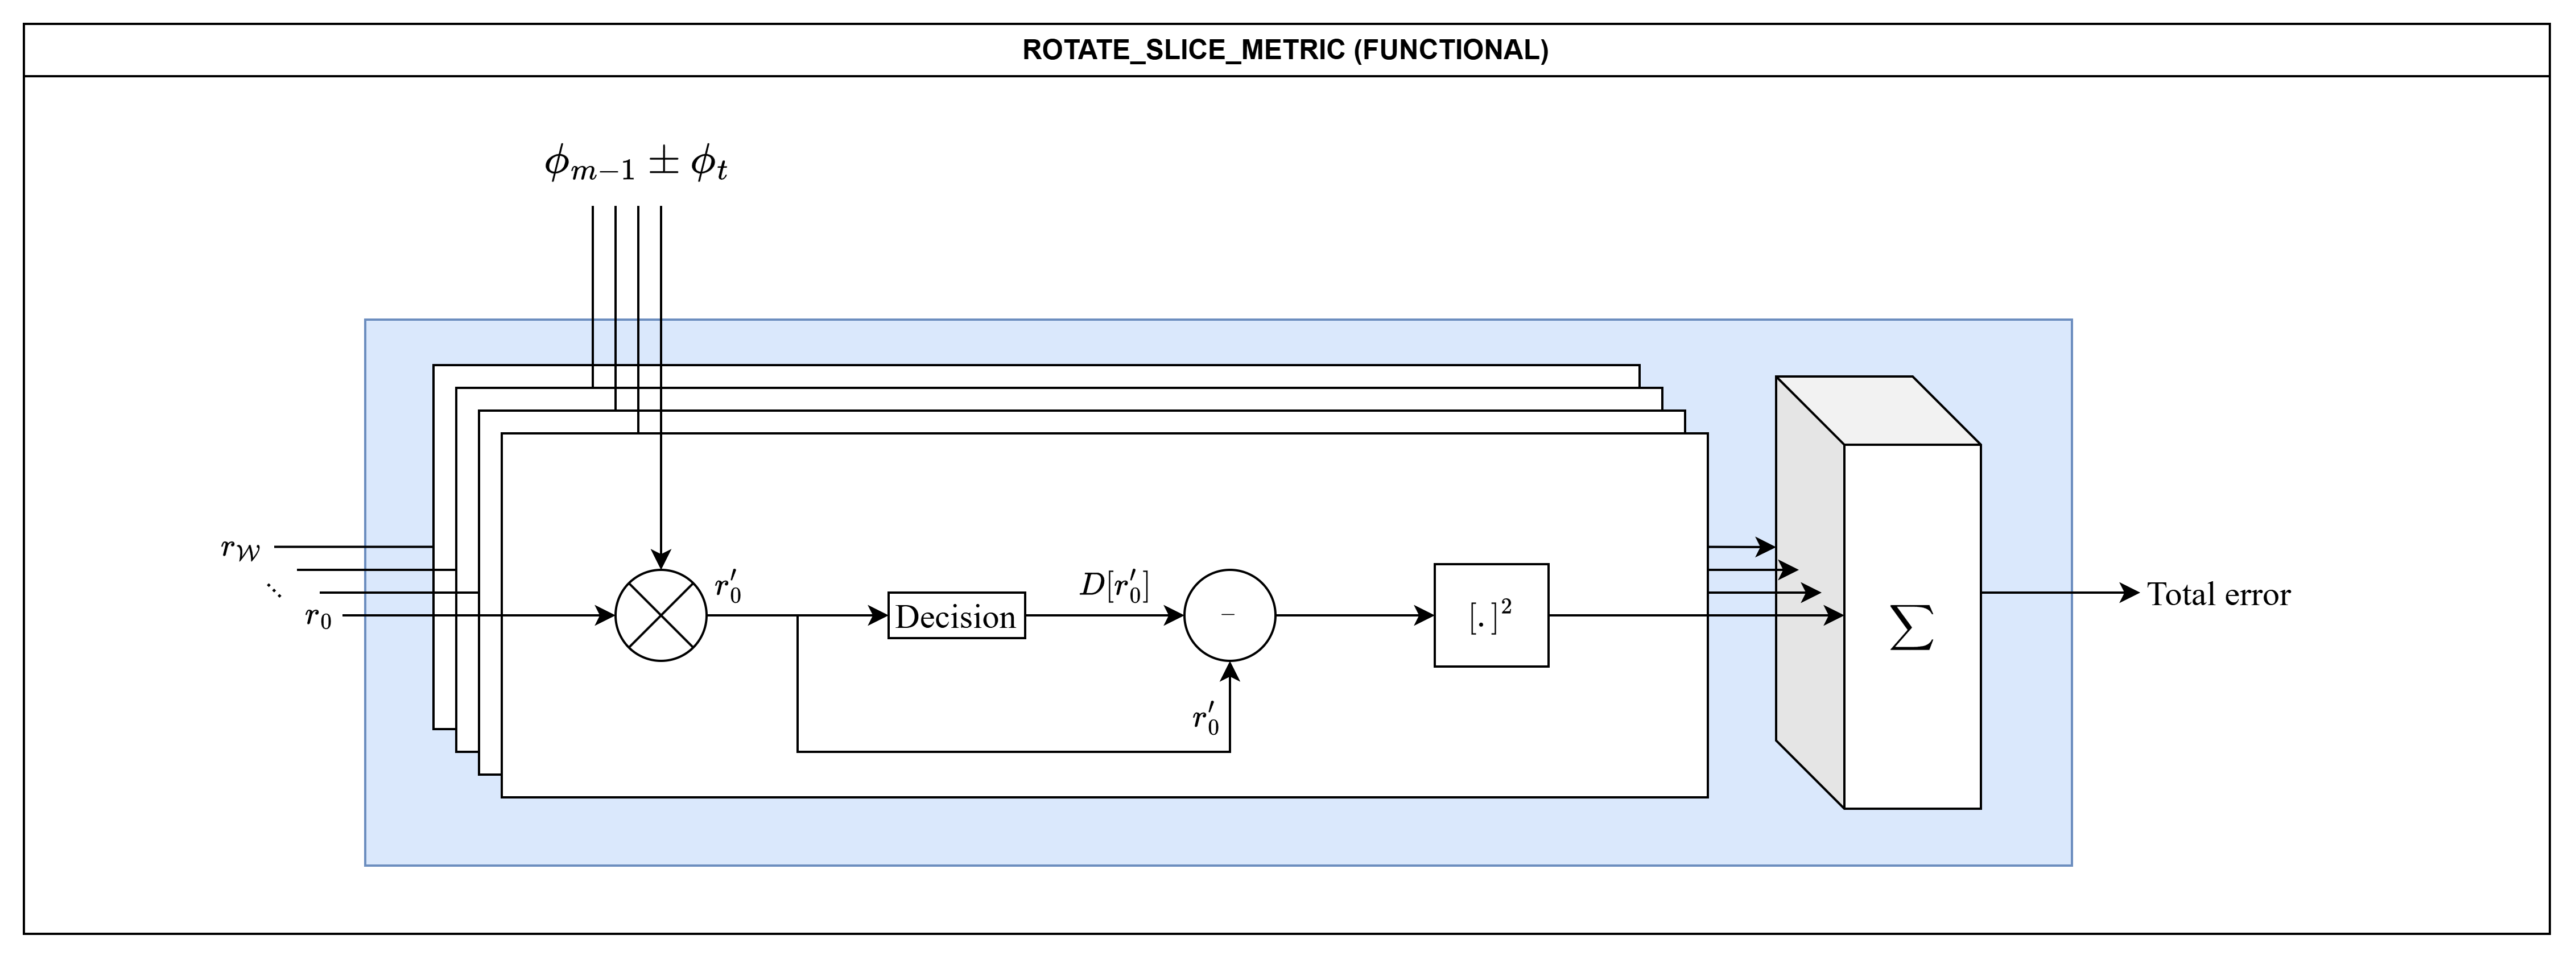
\includegraphics[width=0.8\linewidth]{figures/rotate_slice_metric_functional.png}
\caption{Functional diagram of the \textit{rotate metric slice} unit }
\label{fig:functional-rotate-slice-metric}
\end{figure}

\subsection{Data flow}

The data-oriented view of the implementation is shown in Figs.~\ref{fig:data-SBPS-full}, \ref{fig:data-SBPS-stage}, and \ref{fig:data-rotate-slice-metric}.

\begin{figure}[H]
\centering
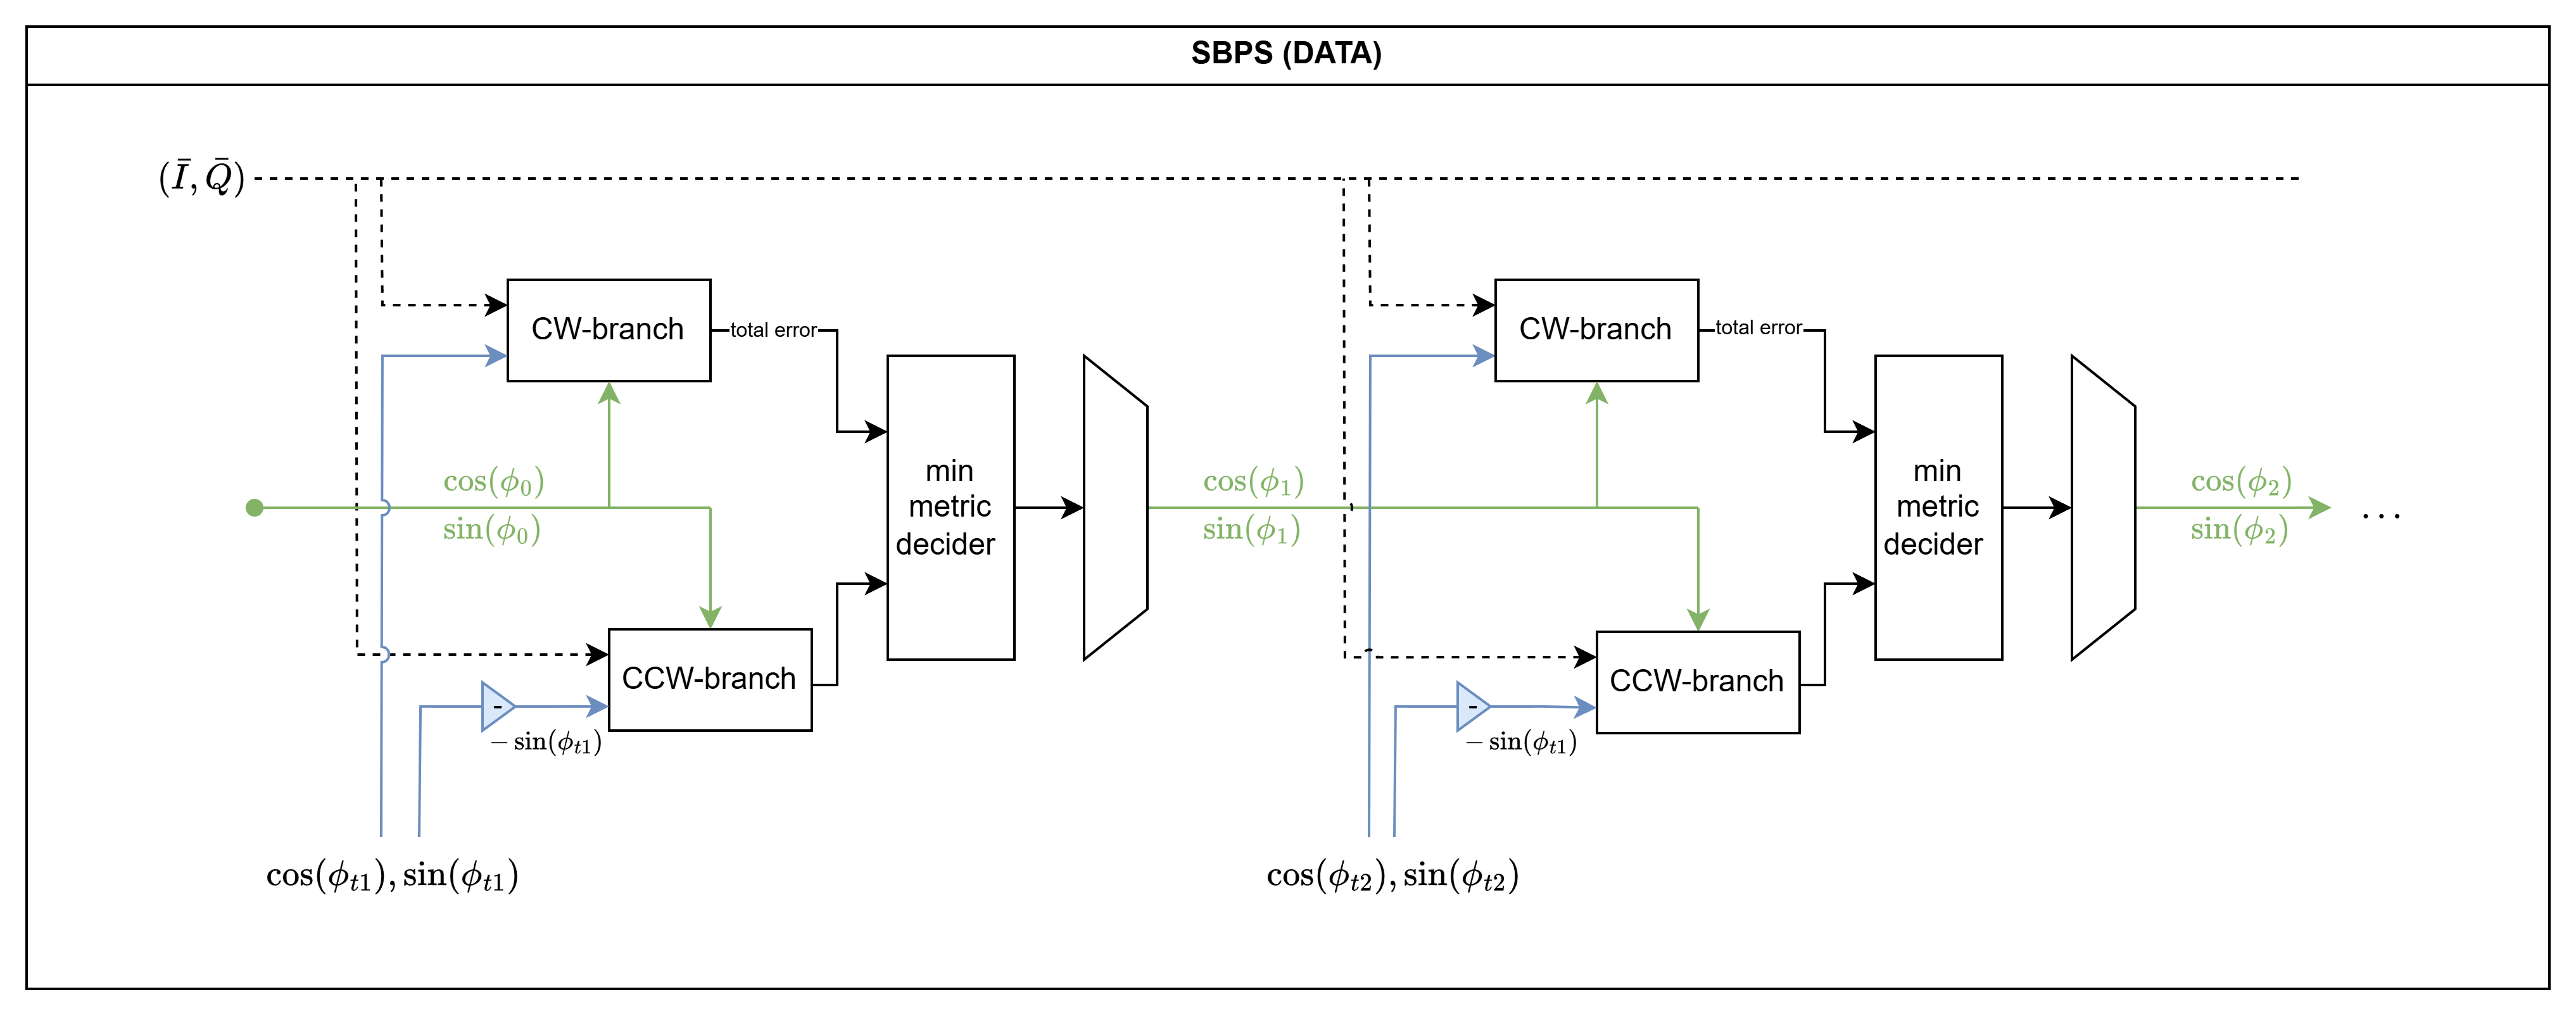
\includegraphics[width=0.8\linewidth]{figures/SBPS_data.png}
\caption{Datapath diagram of the full SBPS architecture}
\label{fig:data-SBPS-full}
\end{figure}


\begin{figure}[H]
\centering
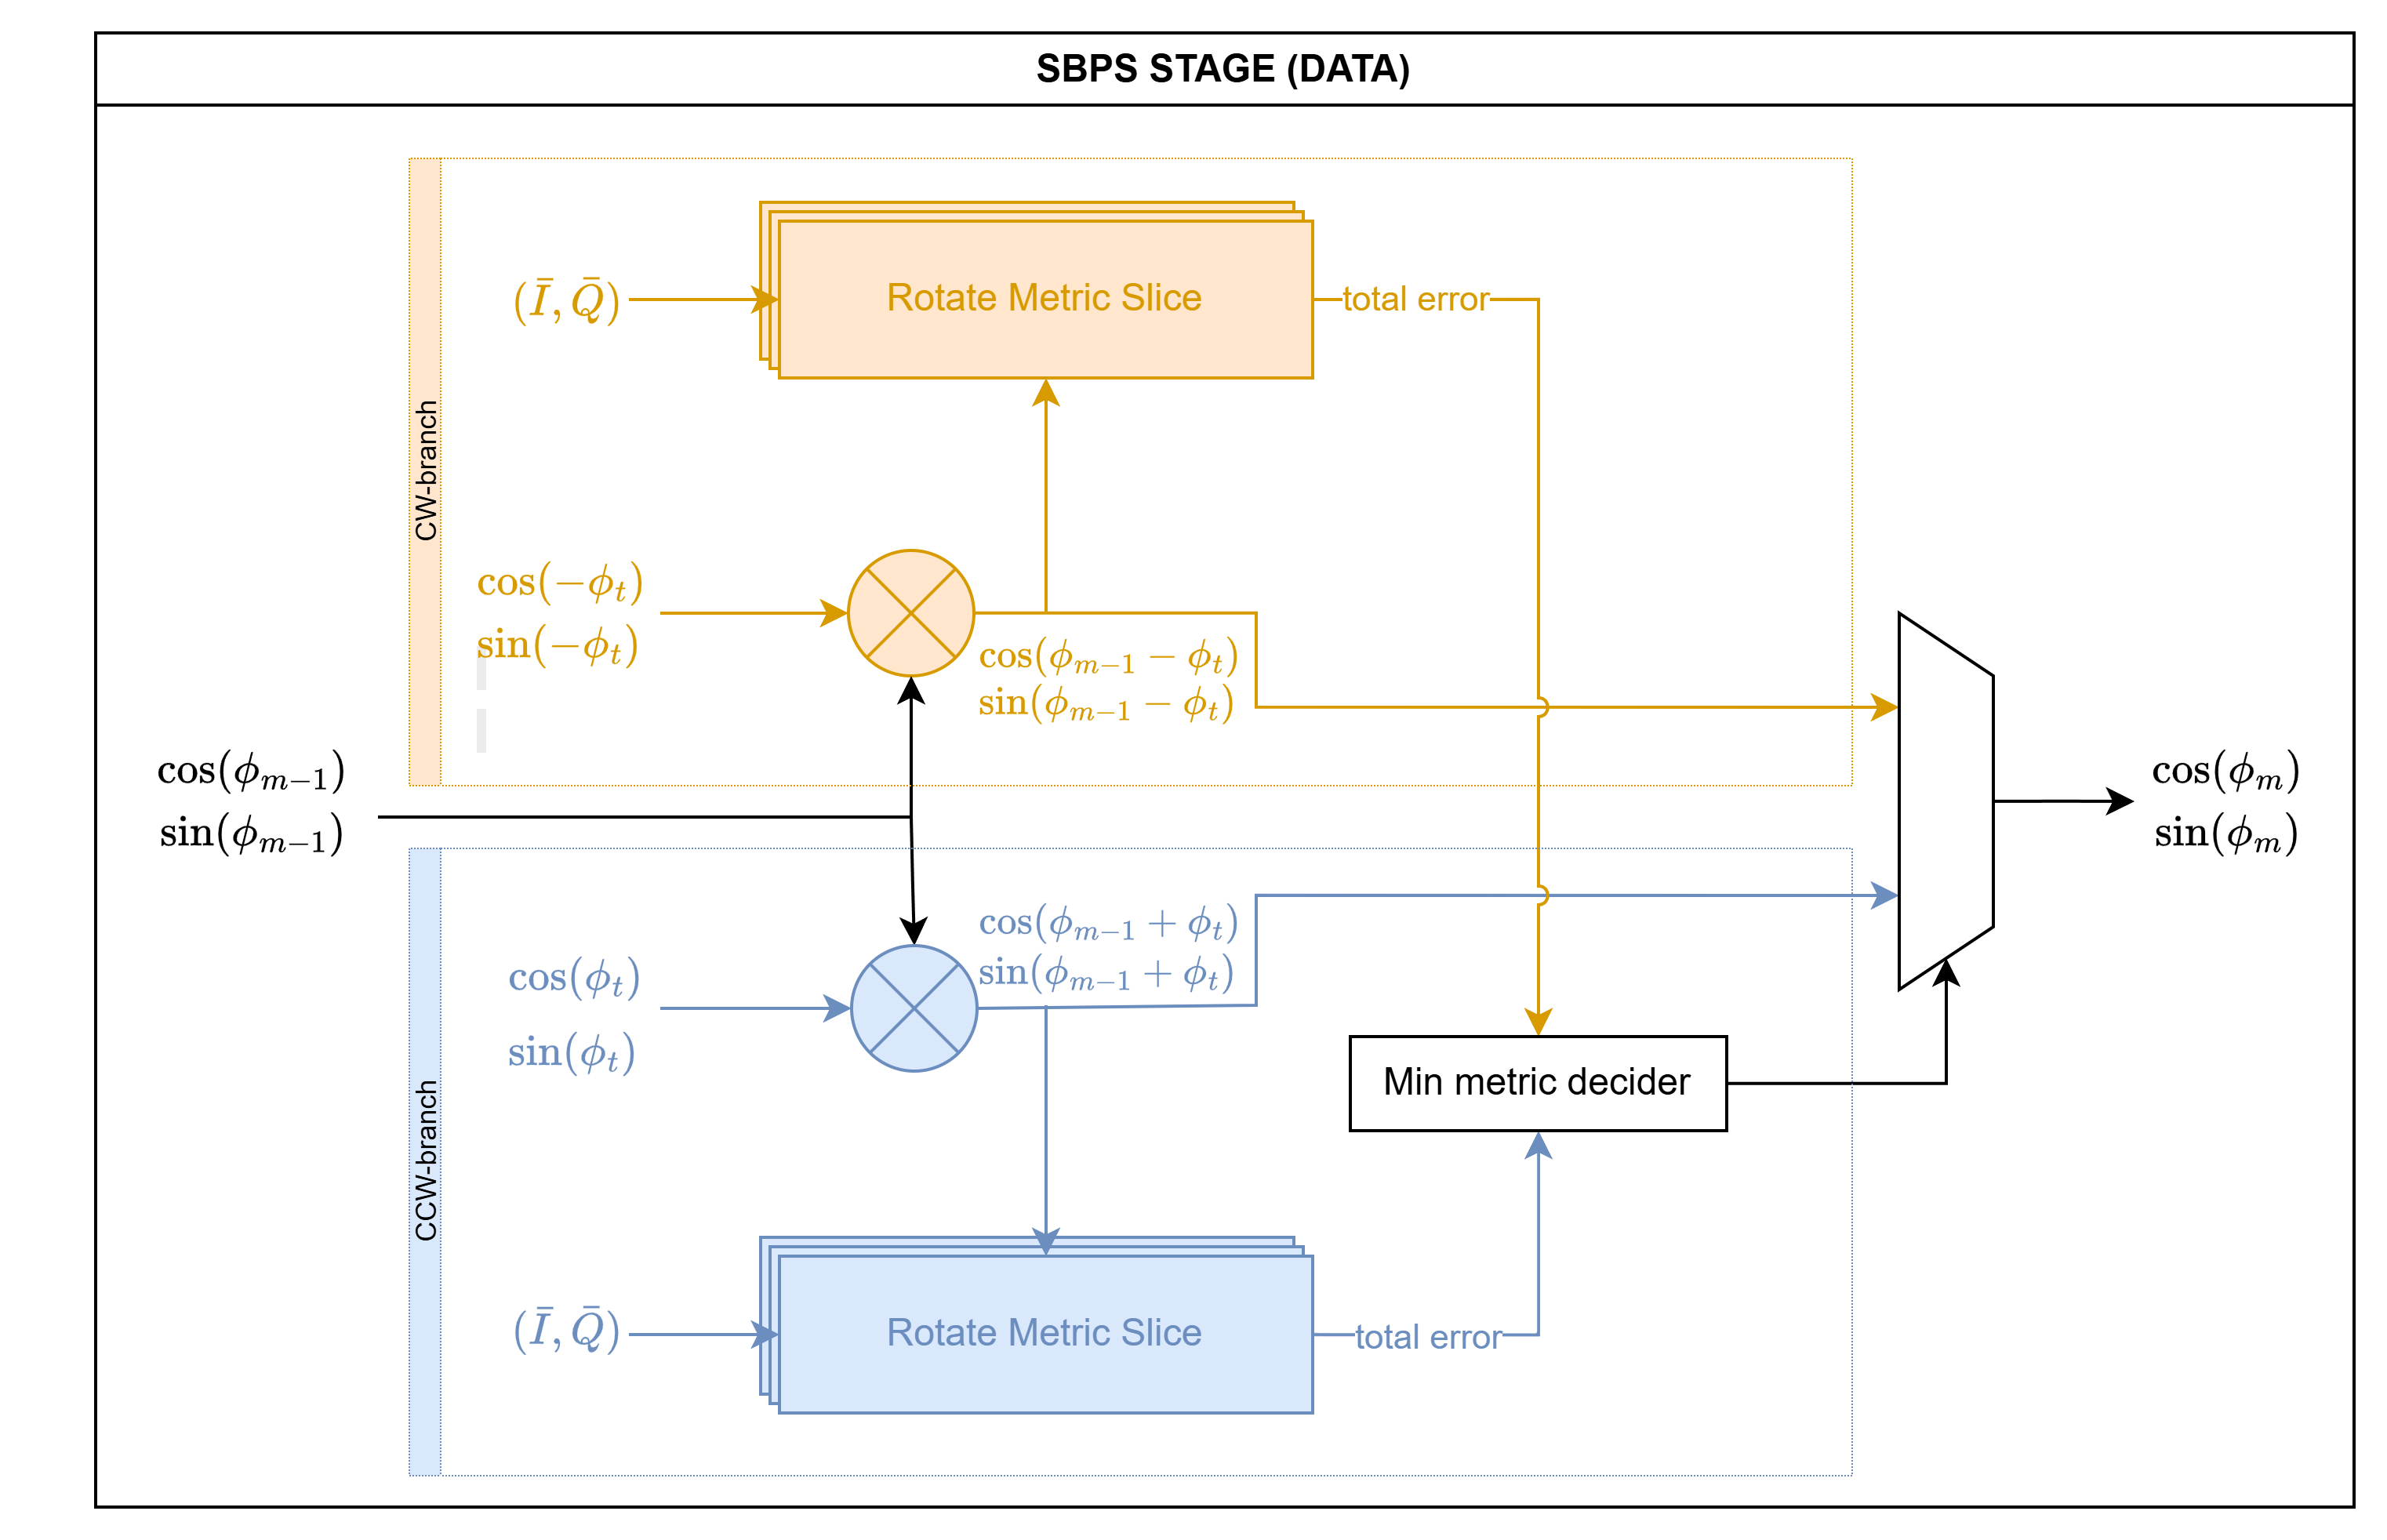
\includegraphics[width=0.8\linewidth]{figures/SBPS_stage_data.png}
\caption{Datapath diagram of the SBPS stage }
\label{fig:data-SBPS-stage}
\end{figure}

In the implemented datapath, phase is not represented as an explicit angle word. Instead, each phase value is carried by its trigonometric components \((\cos(\phi), \sin(\phi))\) in fixed-point format. This allows the candidate phases to be generated directly by the \textit{angle add} block from the previous estimate \((\cos(\phi_{m-1}), \sin(\phi_{m-1}))\) and the stage test angle \((\cos(\phi_t), \sin(\phi_t))\):
\begin{align}
\cos(\phi_{m-1} \pm \phi_t)
&= \cos(\phi_{m-1})\cos(\phi_t) \mp \sin(\phi_{m-1})\sin(\phi_t), \\
\sin(\phi_{m-1} \pm \phi_t)
&= \sin(\phi_{m-1})\cos(\phi_t) \pm \cos(\phi_{m-1})\sin(\phi_t).
\end{align}

Once a candidate phase has been formed, the received samples are rotated in the \(I/Q\) plane. For a candidate angle
\[
\theta \in \left\{\phi_{m-1}-\phi_t,\; \phi_{m-1}+\phi_t\right\},
\]
the rotator computes
\begin{equation}
\label{eq:rotated_samples}
\begin{aligned}
I_k' &= I_k \cos(\theta) + Q_k \sin(\theta), \\
Q_k' &= -I_k \sin(\theta) + Q_k \cos(\theta),
\end{aligned}
\end{equation}
for every symbol \(r_k = I_k + jQ_k\) in the block. The rotated symbol is then denoted by \(r_k' = I_k' + jQ_k'\).

\begin{figure}[H]
\centering
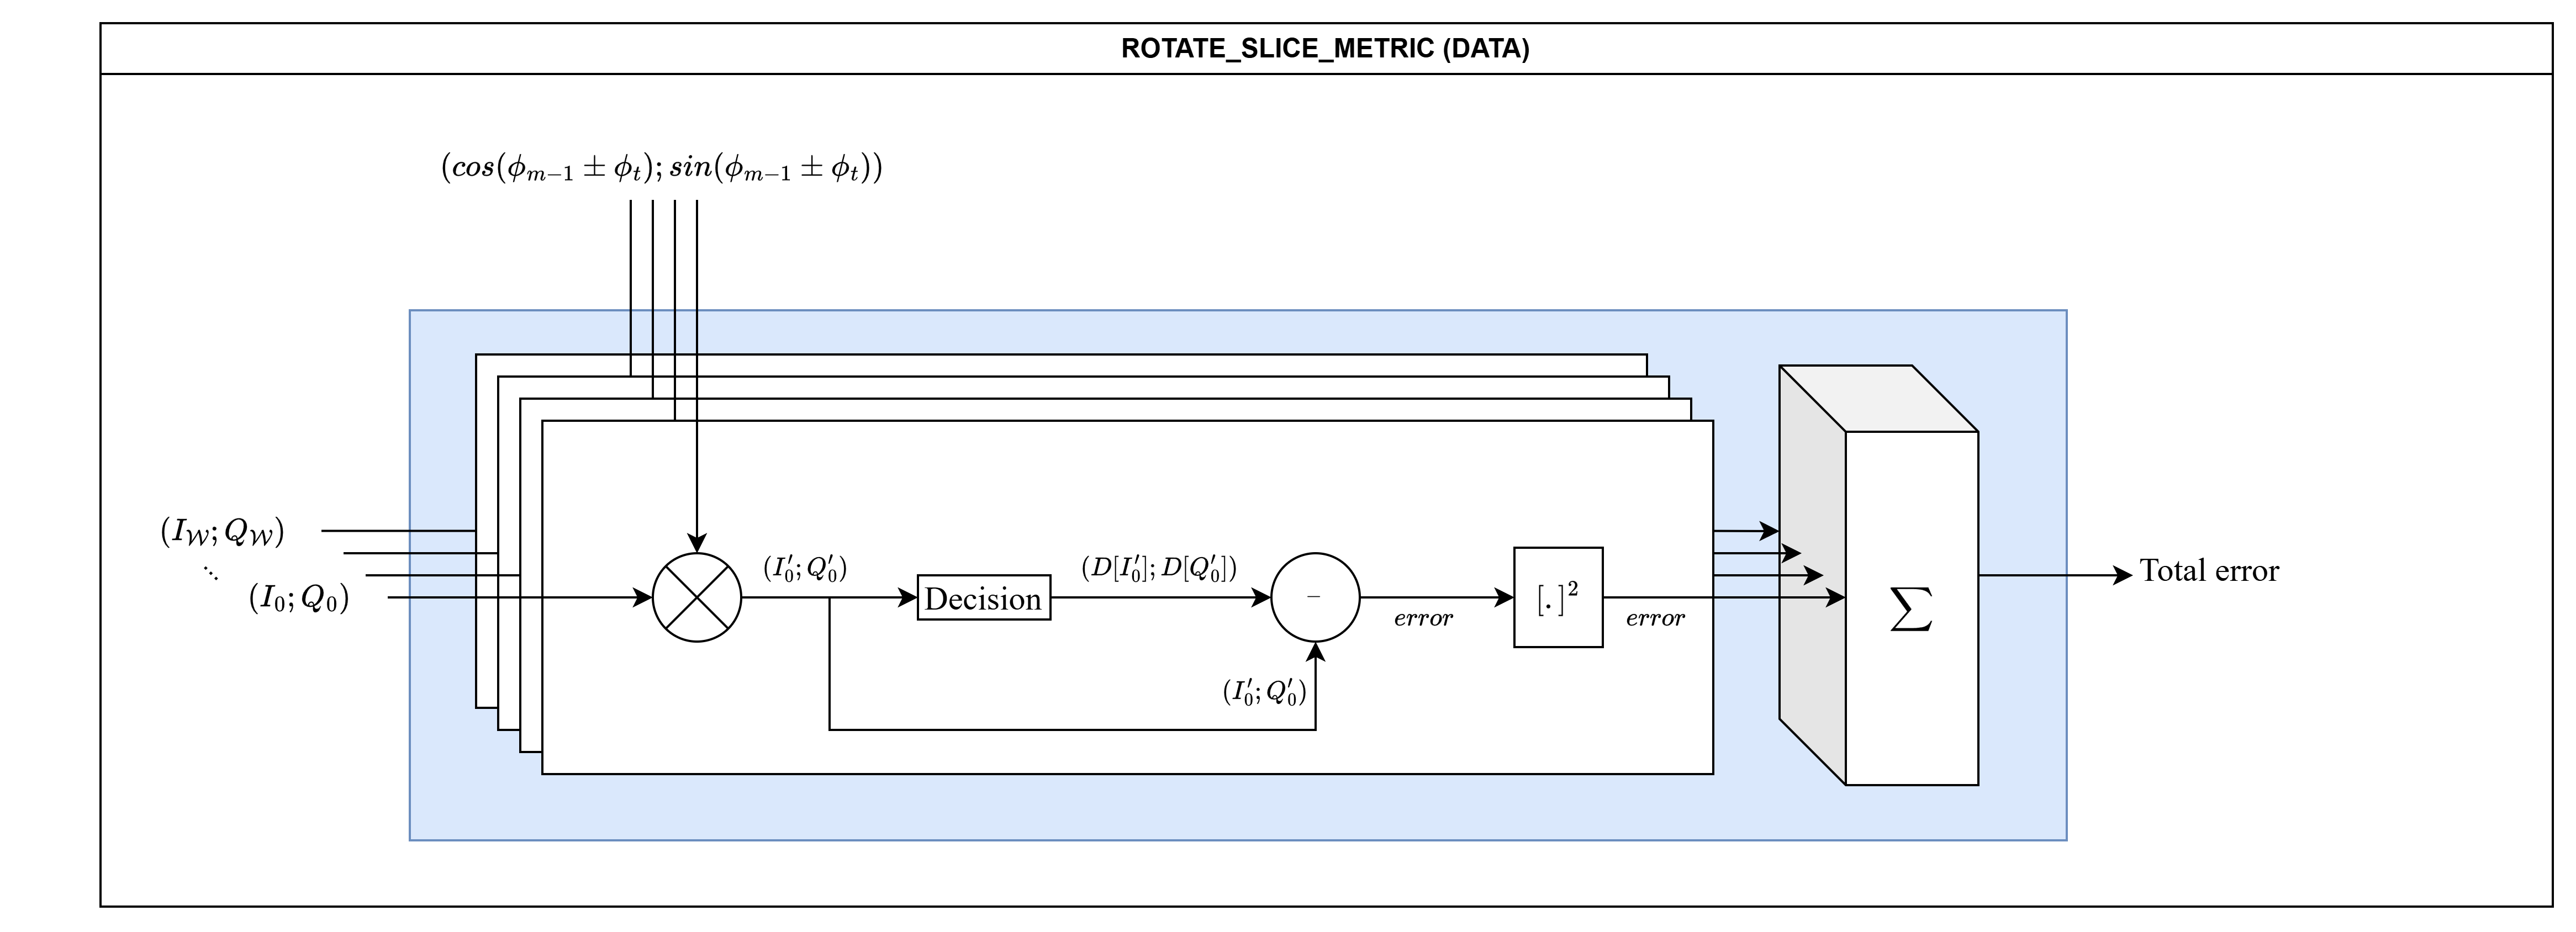
\includegraphics[width=0.8\linewidth]{figures/rotate_slice_metric_data.png}
\caption{Datapath diagram of the \textit{rotate metric slice} unit }
\label{fig:data-rotate-slice-metric}
\end{figure}

For standard 16QAM operation, the slicer maps each rotated sample to the nearest reference point \(D[r_k']\). The axis decisions are derived from the conventional inner--outer thresholds, with \(\pm 2s\) defining the transition between the inner and outer levels of the constellation. The resulting single-symbol error is
\begin{equation}
\label{eq:single-symbol-error}
e_k = \left|r_k' - D[r_k']\right|^2
    = \left(I_k' - D_I[r_k']\right)^2
    + \left(Q_k' - D_Q[r_k']\right)^2,
\end{equation}
and the branch metric is obtained by accumulation over the complete block:
\begin{equation}
E = \sum_{k=0}^{\mathcal W-1} e_k.
\end{equation}
This accumulated metric is the quantity used by the \textit{min metric decider} to select the surviving branch.

\subsection{Timing flow}

The timing behaviour of the full chain, of one SBPS stage, and of the \textit{rotate metric slice} unit is summarised in Figs.~\ref{fig:timing-SBPS-full}, \ref{fig:timing-SBPS-stage}, and \ref{fig:timing_rotate_metric_slice}, respectively. The control path uses single-cycle valid pulses rather than a ready/valid handshake, so temporal alignment is achieved entirely through fixed pipeline delays.

\begin{figure}[H]
\centering
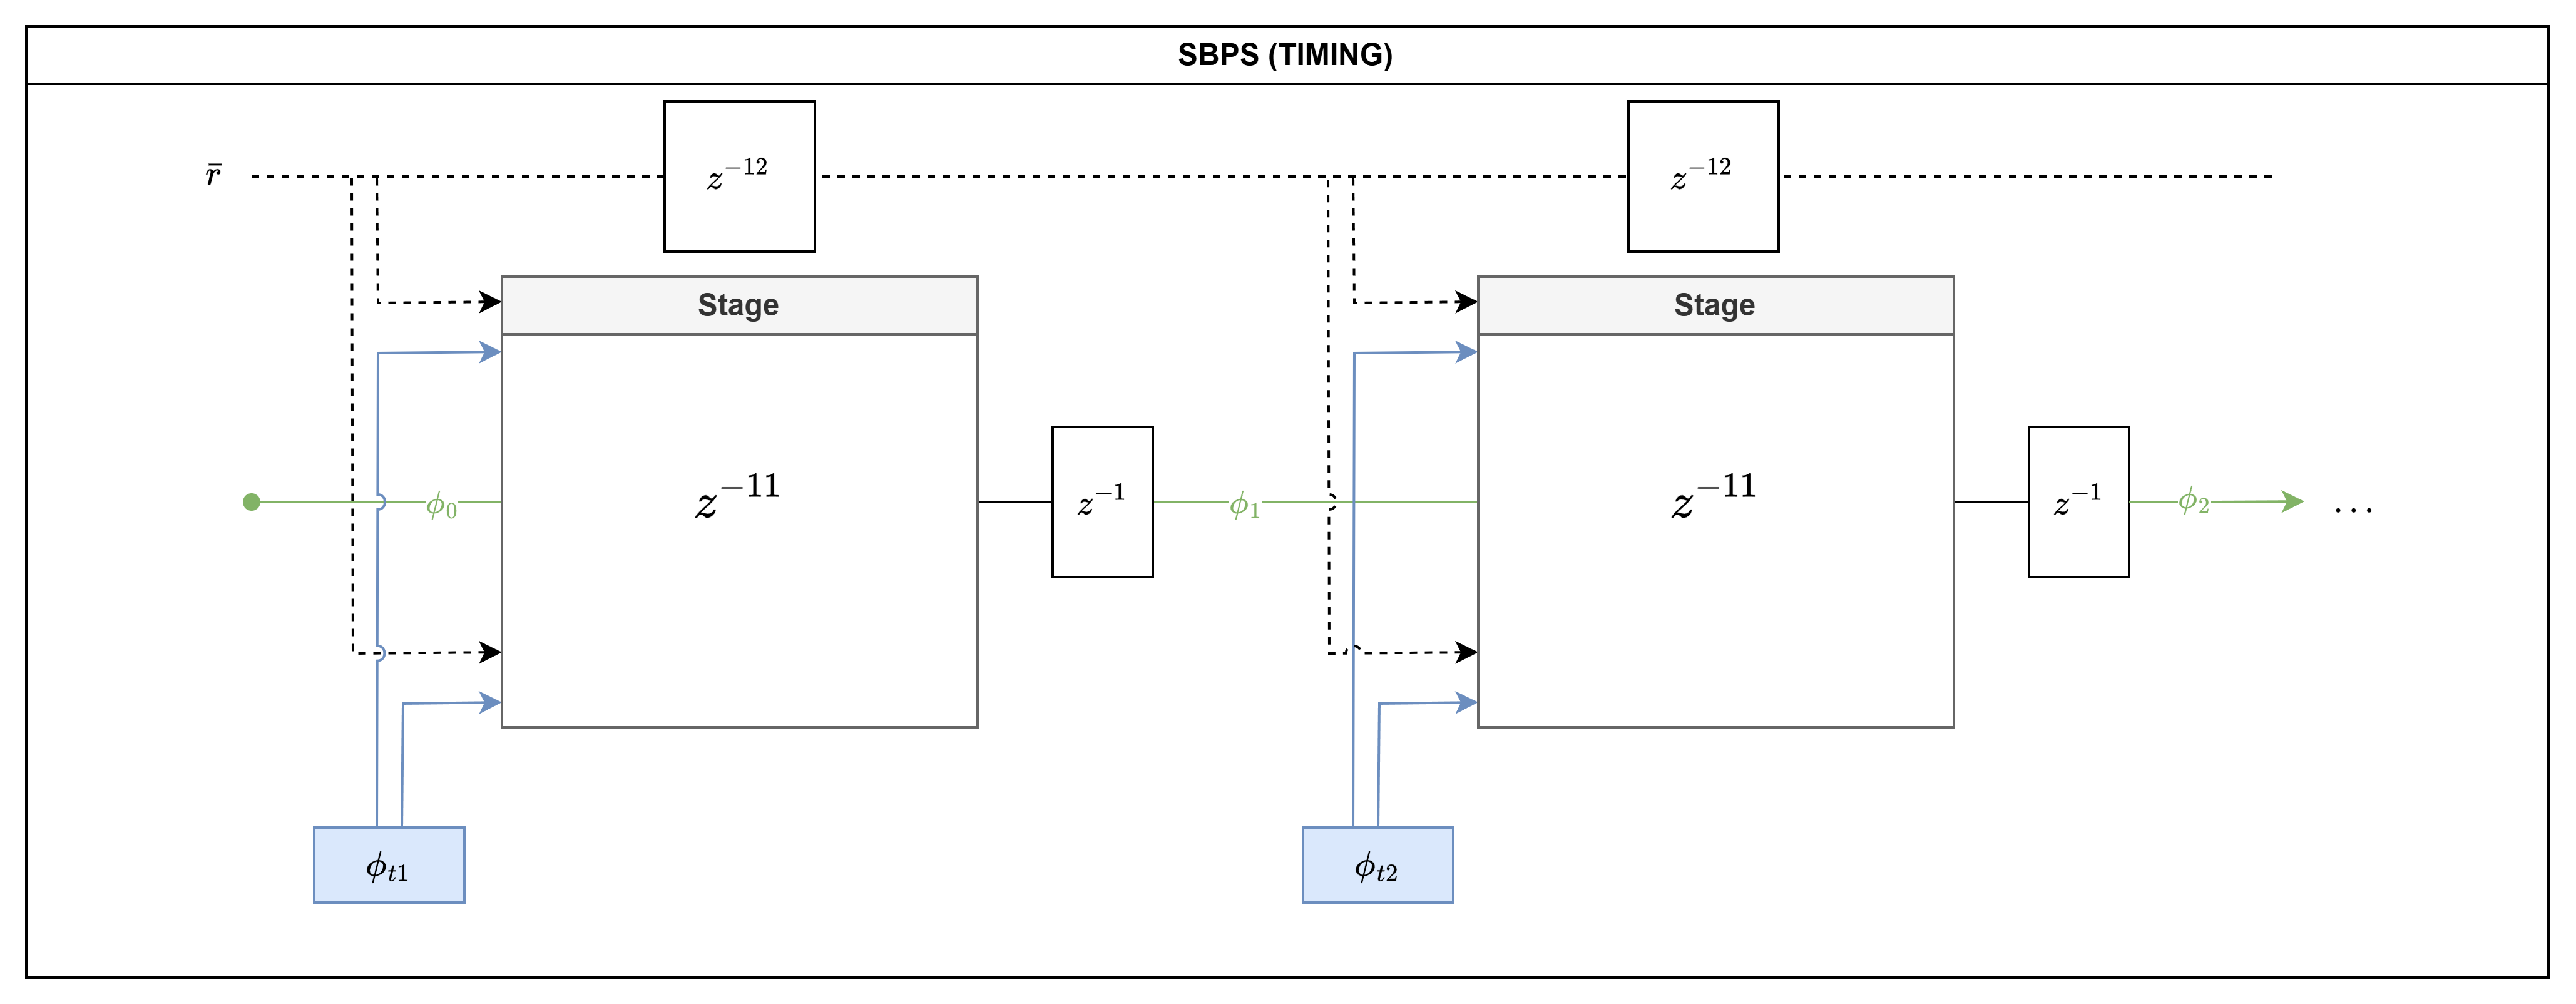
\includegraphics[width=0.8\linewidth]{figures/SBPS_timing.png}
\caption{Timing diagram of the full SBPS algorithm}
\label{fig:timing-SBPS-full}
\end{figure}

At the stage input, the two candidate phases are first generated while the input sample block is delayed in parallel so that both reach the branch datapaths in synchrony. The \textit{angle add} operation introduces three elapsed clock cycles, and the sample block is delayed by the same amount before it enters the \textit{rotate metric slice} unit.

\begin{figure}[H]
\centering
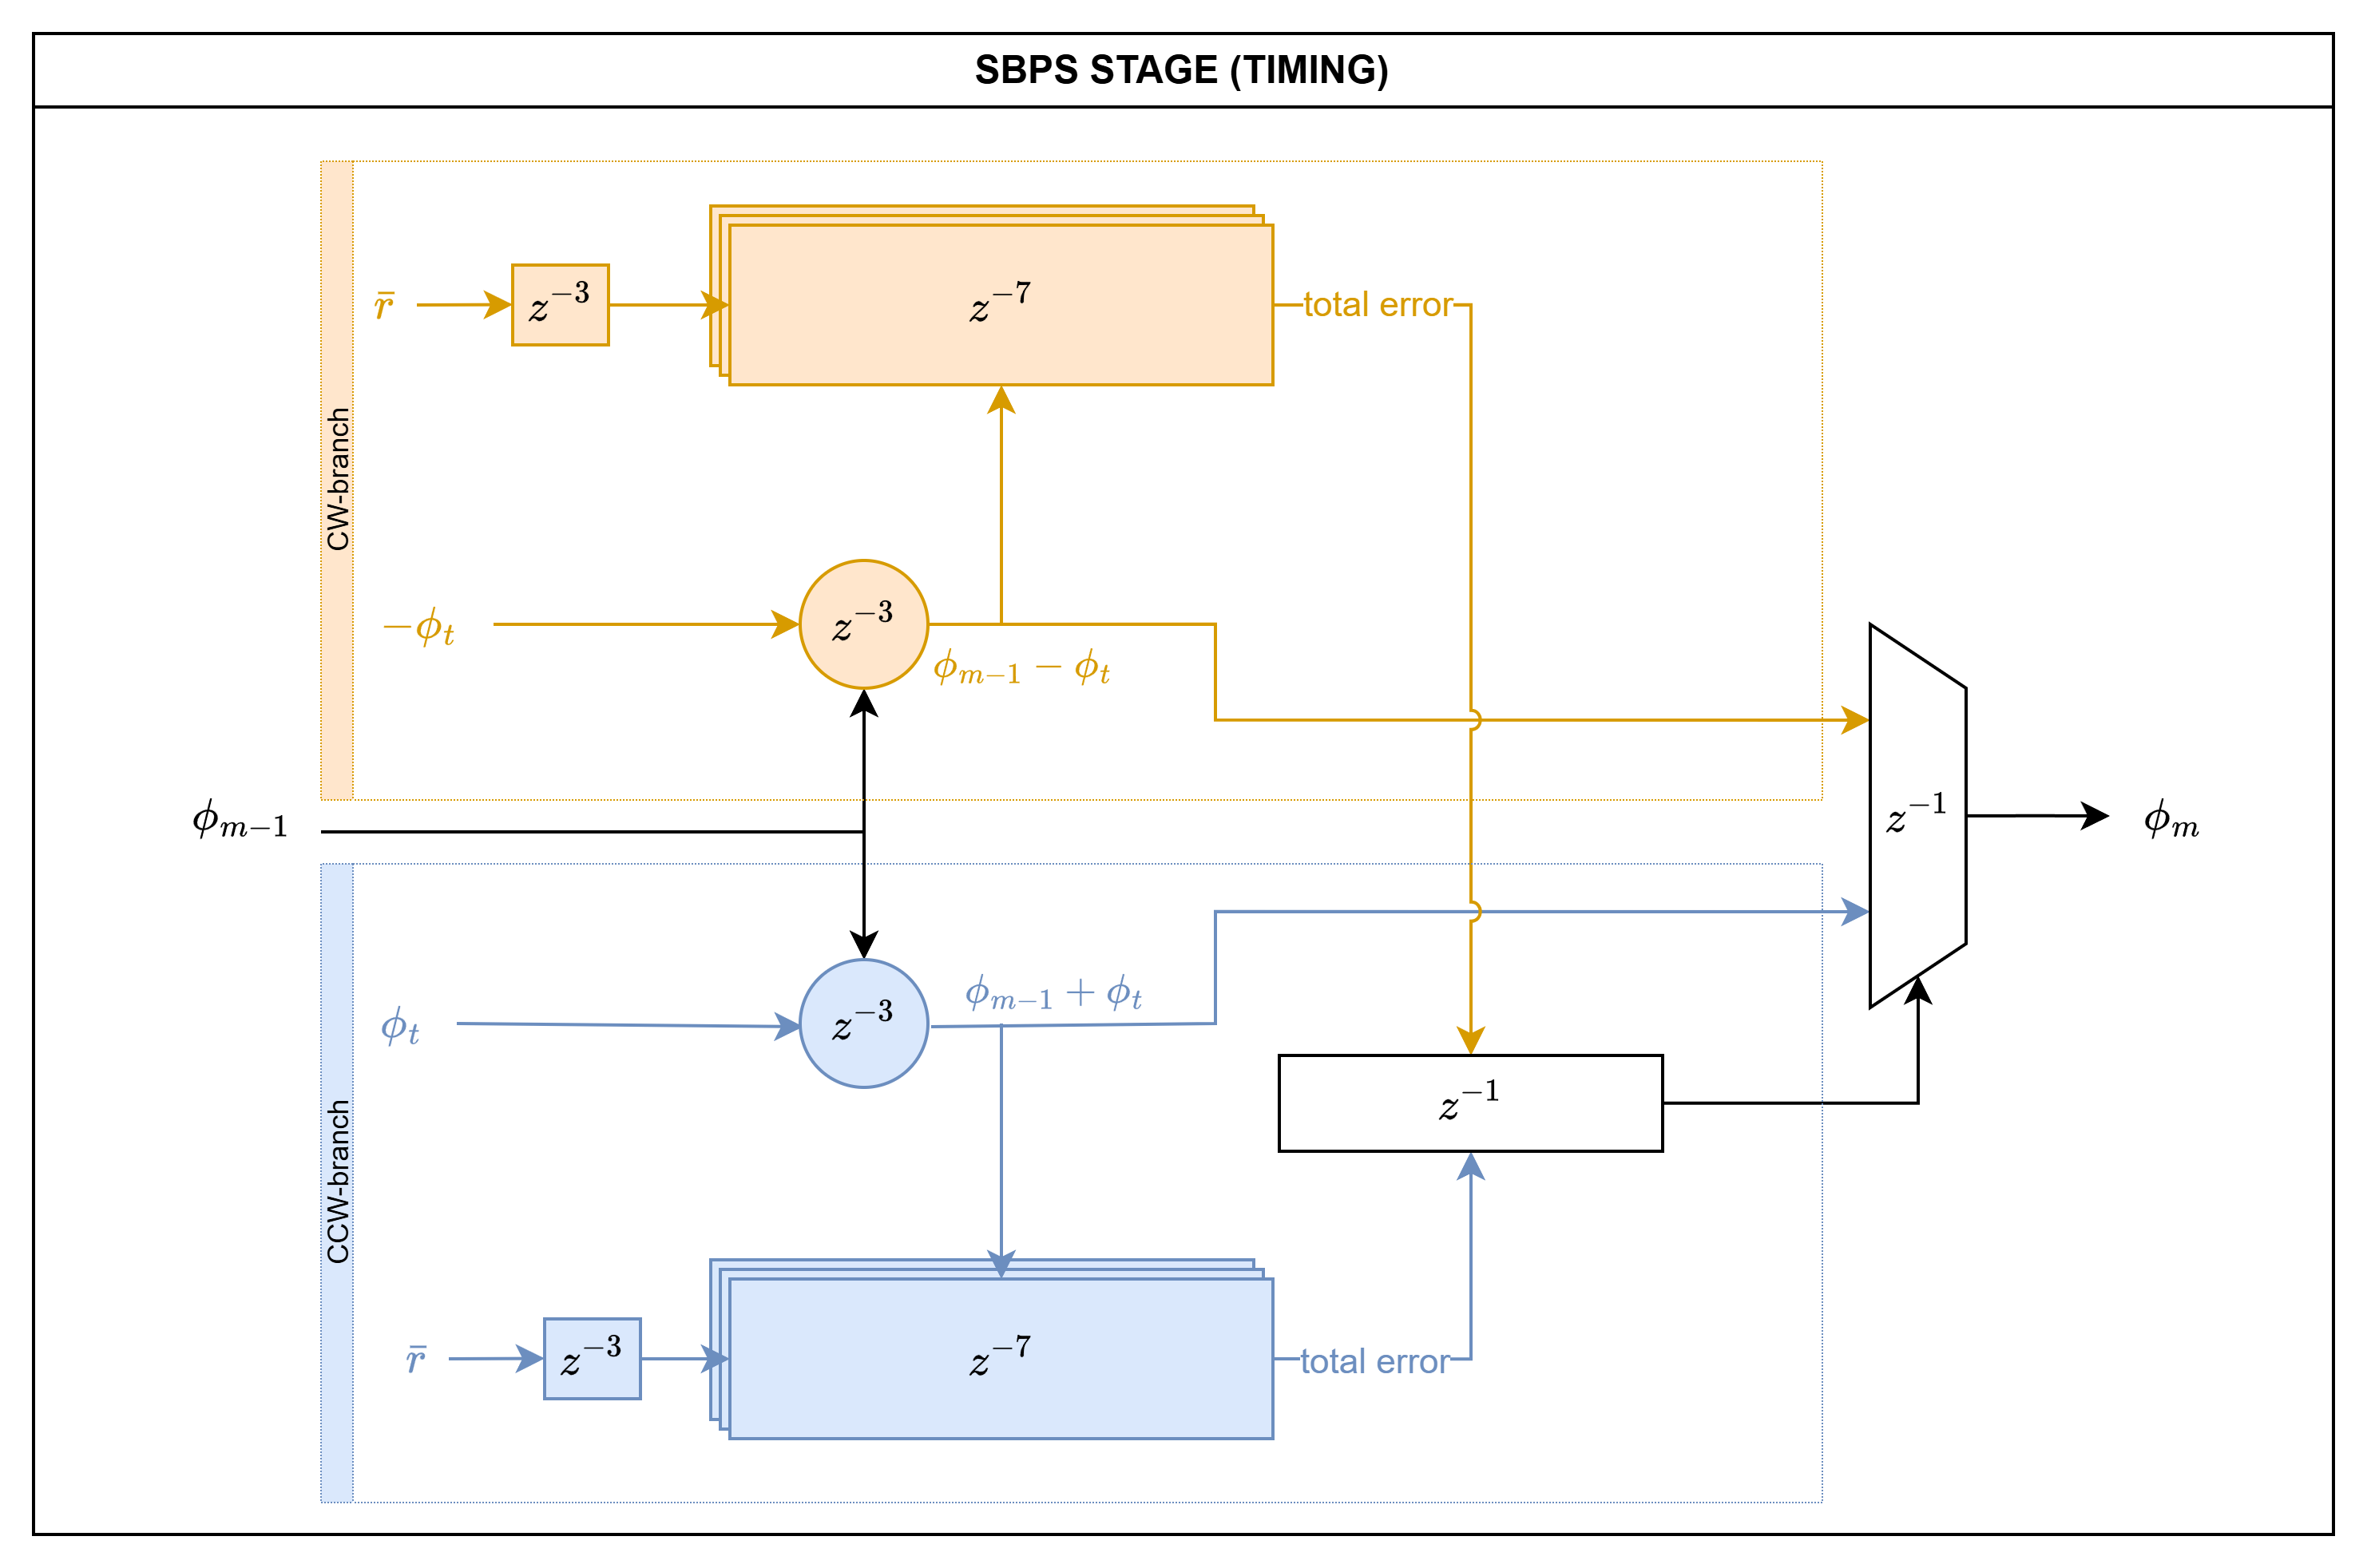
\includegraphics[width=0.8\linewidth]{figures/SBPS_stage_timing.png}
\caption{Timing diagram of the SBPS stage}
\label{fig:timing-SBPS-stage}
\end{figure}

Inside the \textit{rotate metric slice} unit, the rotator contributes three cycles, the slicer and sample-alignment logic contribute one cycle, the single-symbol metric calculation contributes one cycle, and the summation plus output registration contribute two further cycles. The branch metric is therefore available seven cycles after entry into the \textit{rotate metric slice} unit, or ten elapsed cycles after the stage launch when the initial angle-generation and input-alignment delay are included.

\begin{figure}[H]
\centering
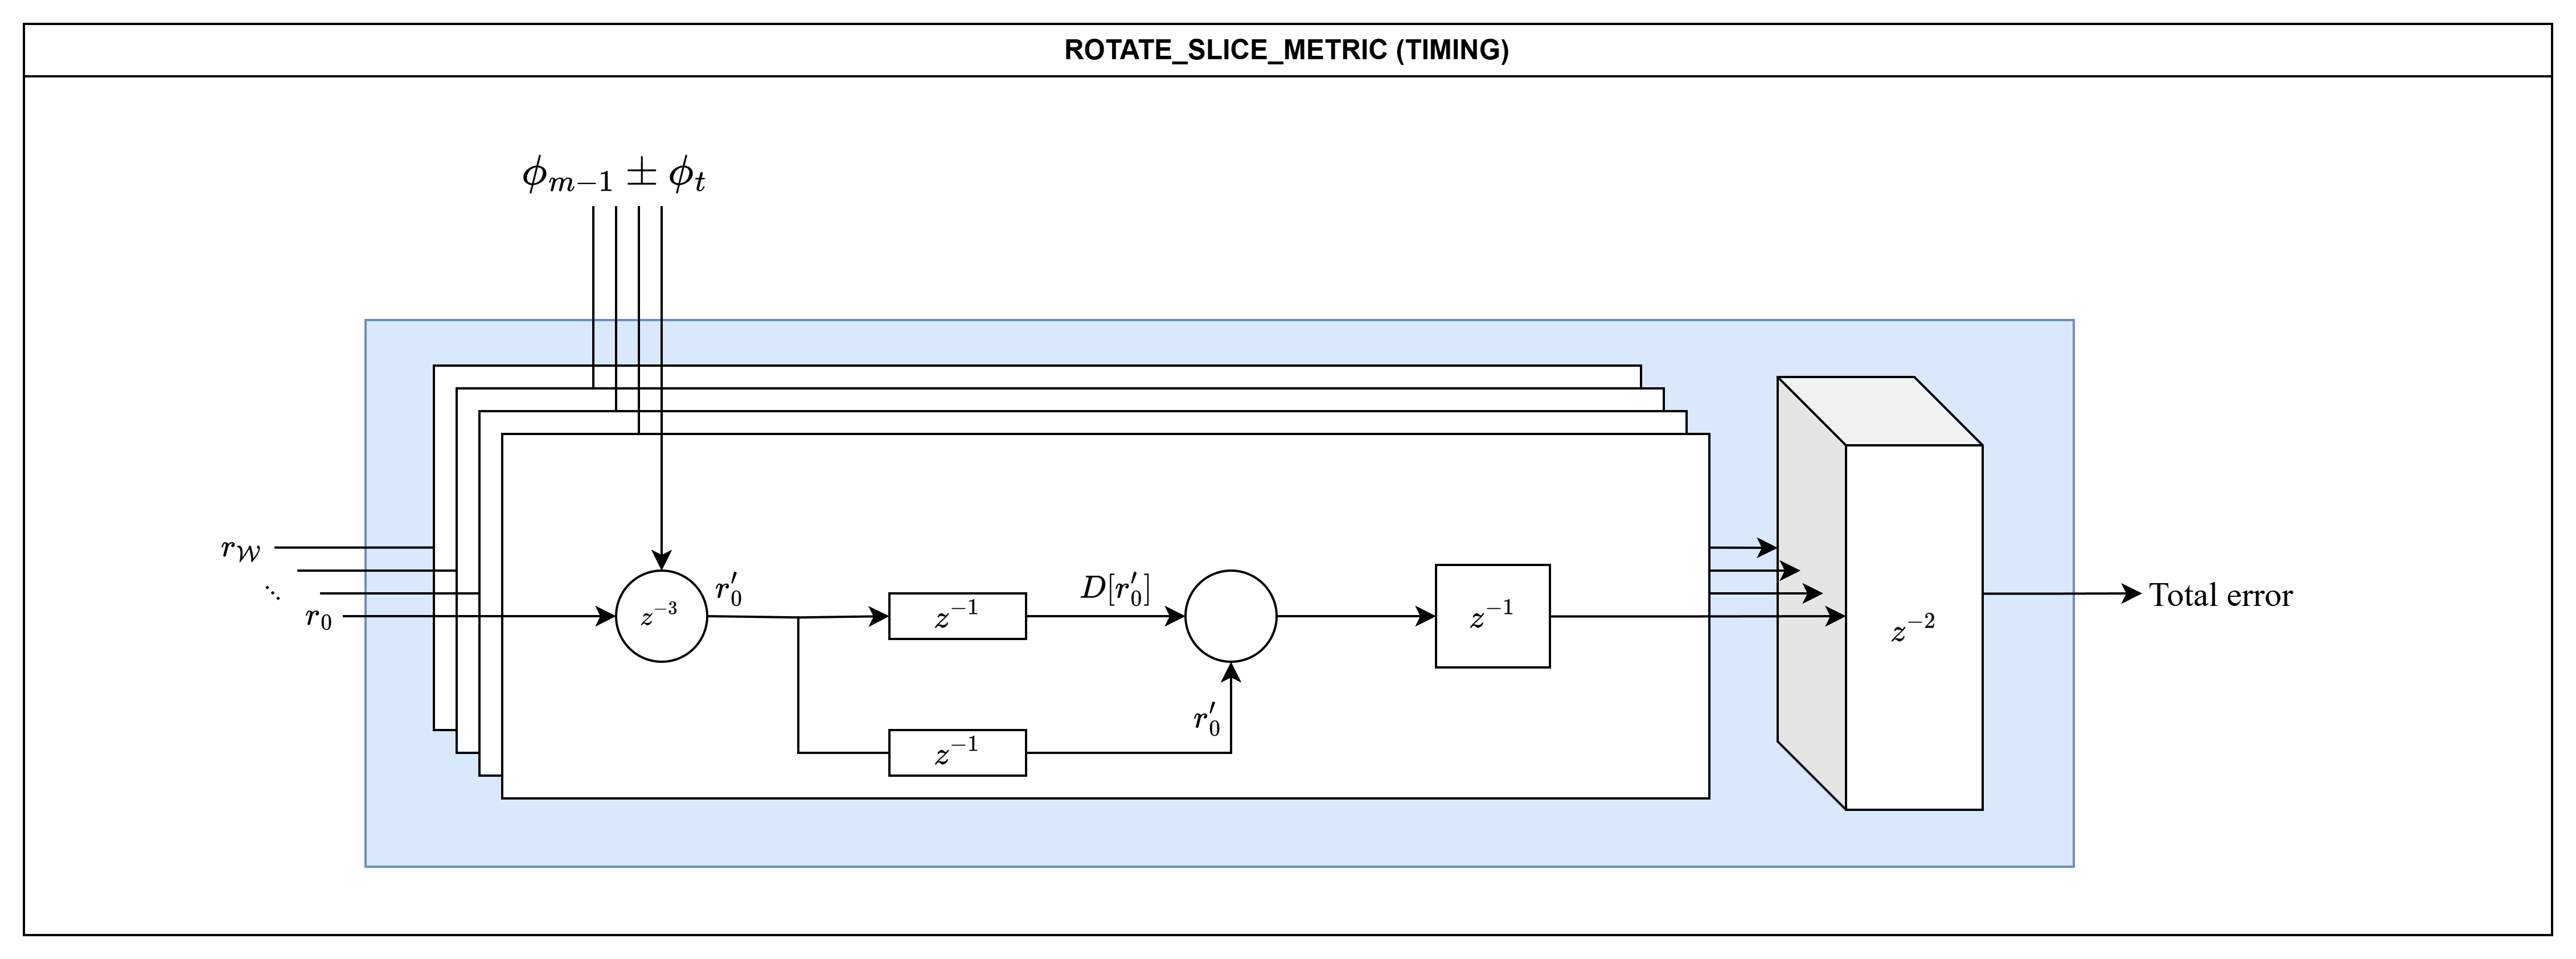
\includegraphics[width=0.8\linewidth]{figures/rotate_slice_metric_timing.png}
\caption{Timing diagram of the \textit{rotate metric slice} unit  }
\label{fig:timing_rotate_metric_slice}
\end{figure}

After both branch metrics have become available, the \textit{min metric decider} requires one clock cycle to determine the winning branch, and the final stage output is registered one cycle later. Consequently, the phase-selection datapath of a stage spans eleven clock cycles, while the registered stage-valid output is asserted after twelve clock cycles. When latency is reported at the boundary of the complete SBPS chain rather than at a single stage boundary, one additional launch cycle must be included because the top-level chain registers the hand-off into the first stage.

\subsection{16QAM-specific adaptations}

For 16QAM, the slicer supports both conventional axis-based decisions and an optional radius-directed mode in the early refinement stages. In the conventional case, the decision on each axis is determined by the inner--outer threshold at \(\pm 2s\). In the radius-directed variant, an additional threshold \(l\) is introduced to identify samples that should be mapped directly to the outer ring of the constellation. This is beneficial in the first stages of the search, where the residual phase uncertainty is still relatively large and a purely axis-based decision can be less reliable. Once the phase estimate has been sufficiently refined, the later stages revert to the standard 16QAM slicer, so that the final metric evaluation follows the nominal decision regions.
\todo{not well enough explained}

% -------------------------------------------------------------
% SPREAD ESTIMATION
% -------------------------------------------------------------
\section{Spread estimation block}
The hardware implementation is split up in the different operational sections of the algorithm, namely the input selector (1), fourth-power demodulators (2), the spread estimator (3), the sign estimator (4) and finally the filters (5). 
The layout of these modules and their relative position is illustrated on Fig~\ref{fig:SE-top}. 
Each section will individually discuss the modules in terms of its functional operation, dataflow and timing flow in order to get a clearer picture of the RTL implementation.

\begin{figure}[H]
\centering
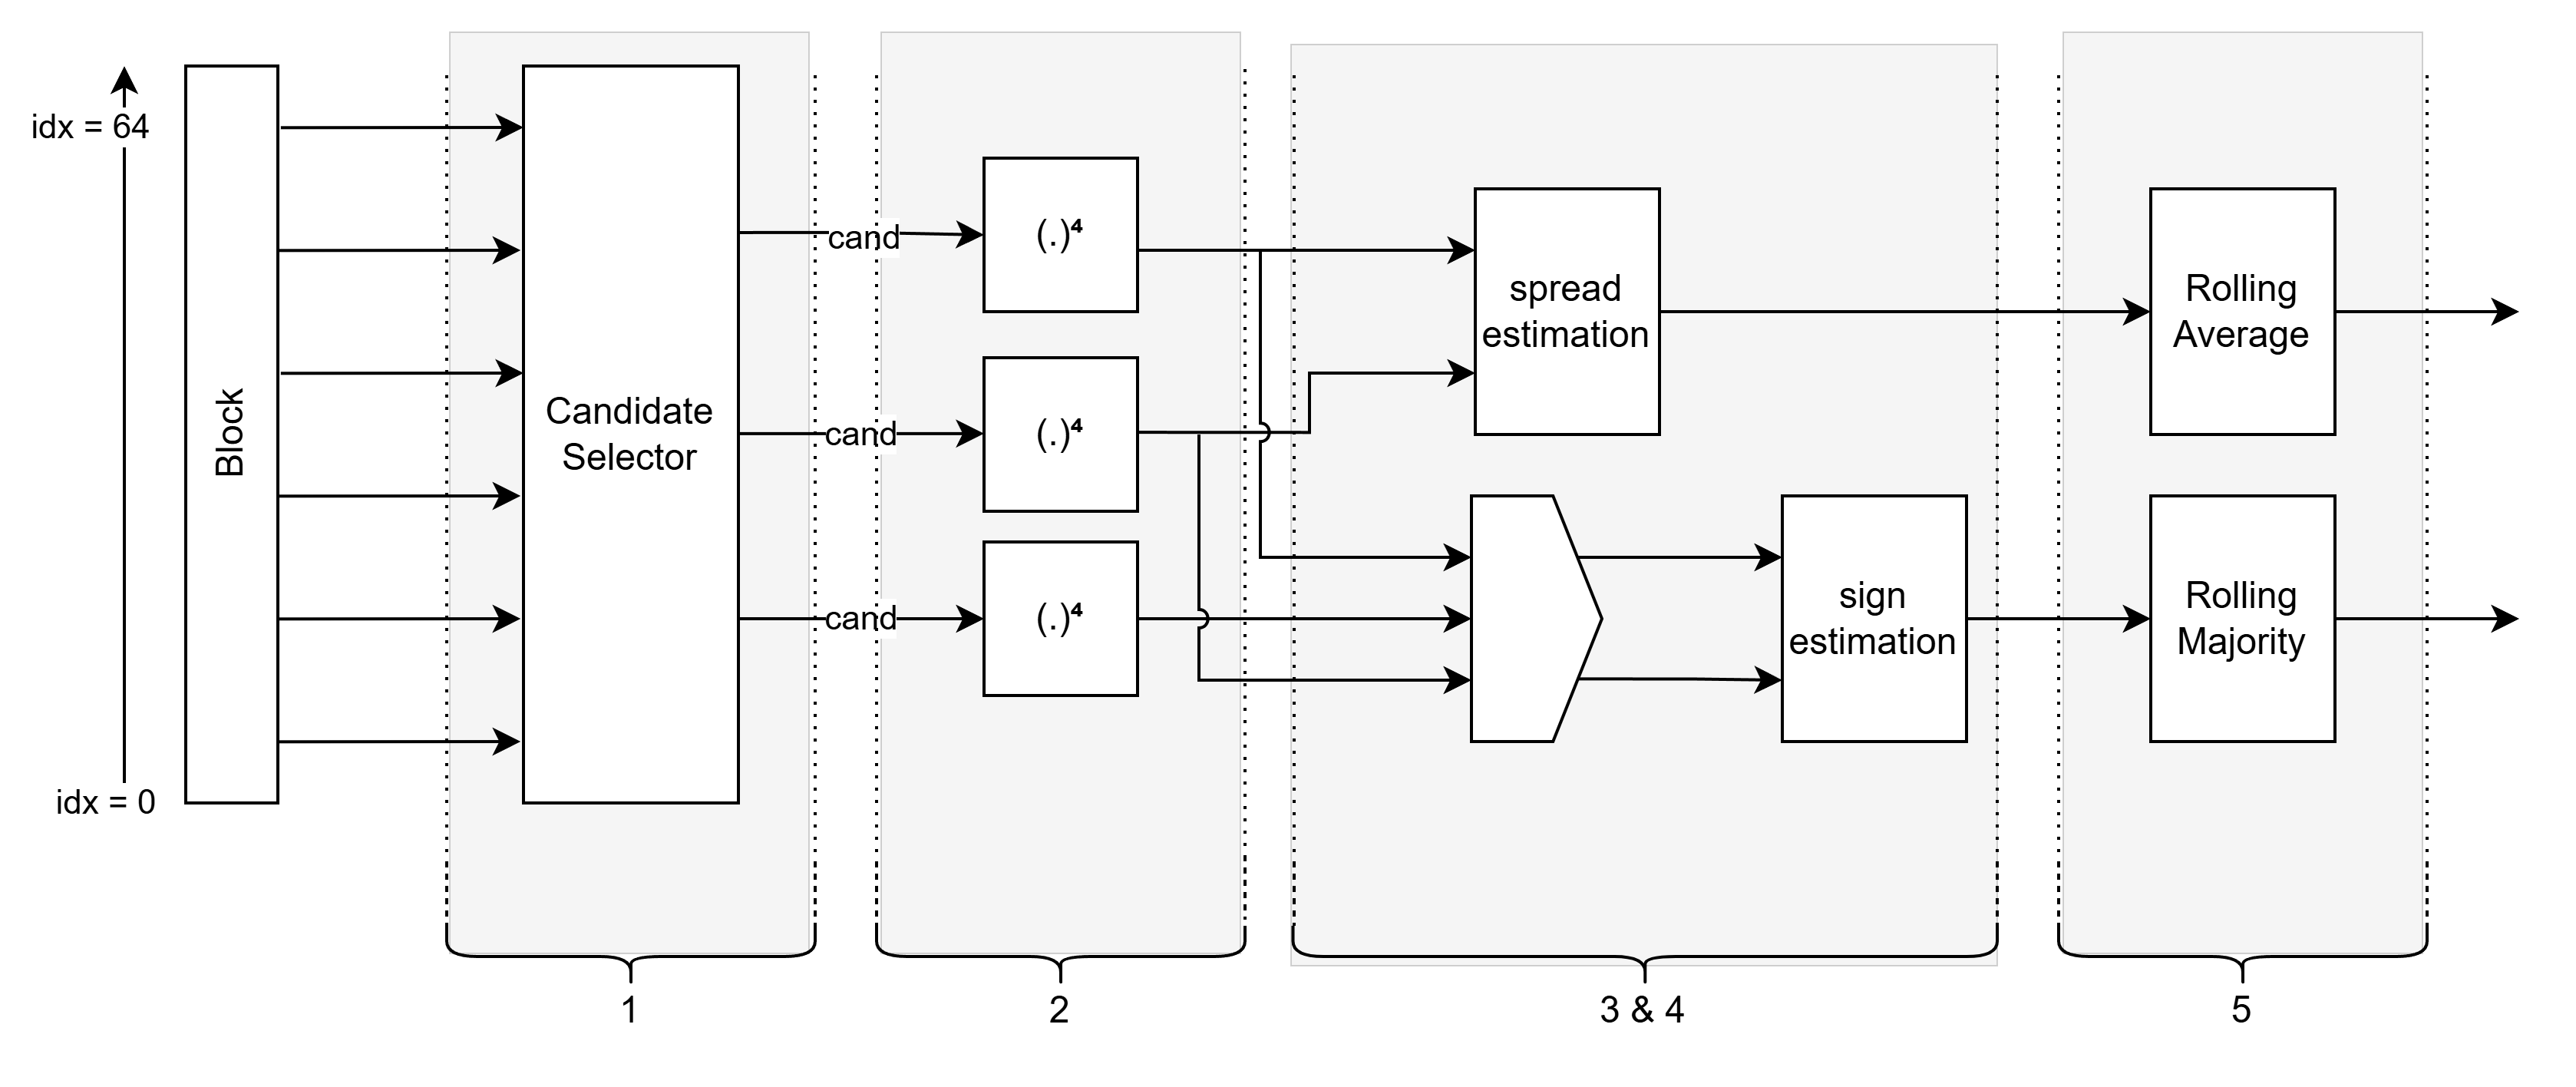
\includegraphics[width=1\linewidth]{figures/SE-top.png}
\caption{Top lay-out of SE block}
\label{fig:SE-top}
\end{figure}

% \subsection{Input selector}
% \subsubsection{Functional operation}
% As discussed in section~\ref{input selector}, before any spread or sign calculation can happen, the input symbols that are fed into the estimators need to be filtered for 
% adequate symbols. 

% \begin{figure}[H]
% \centering
% 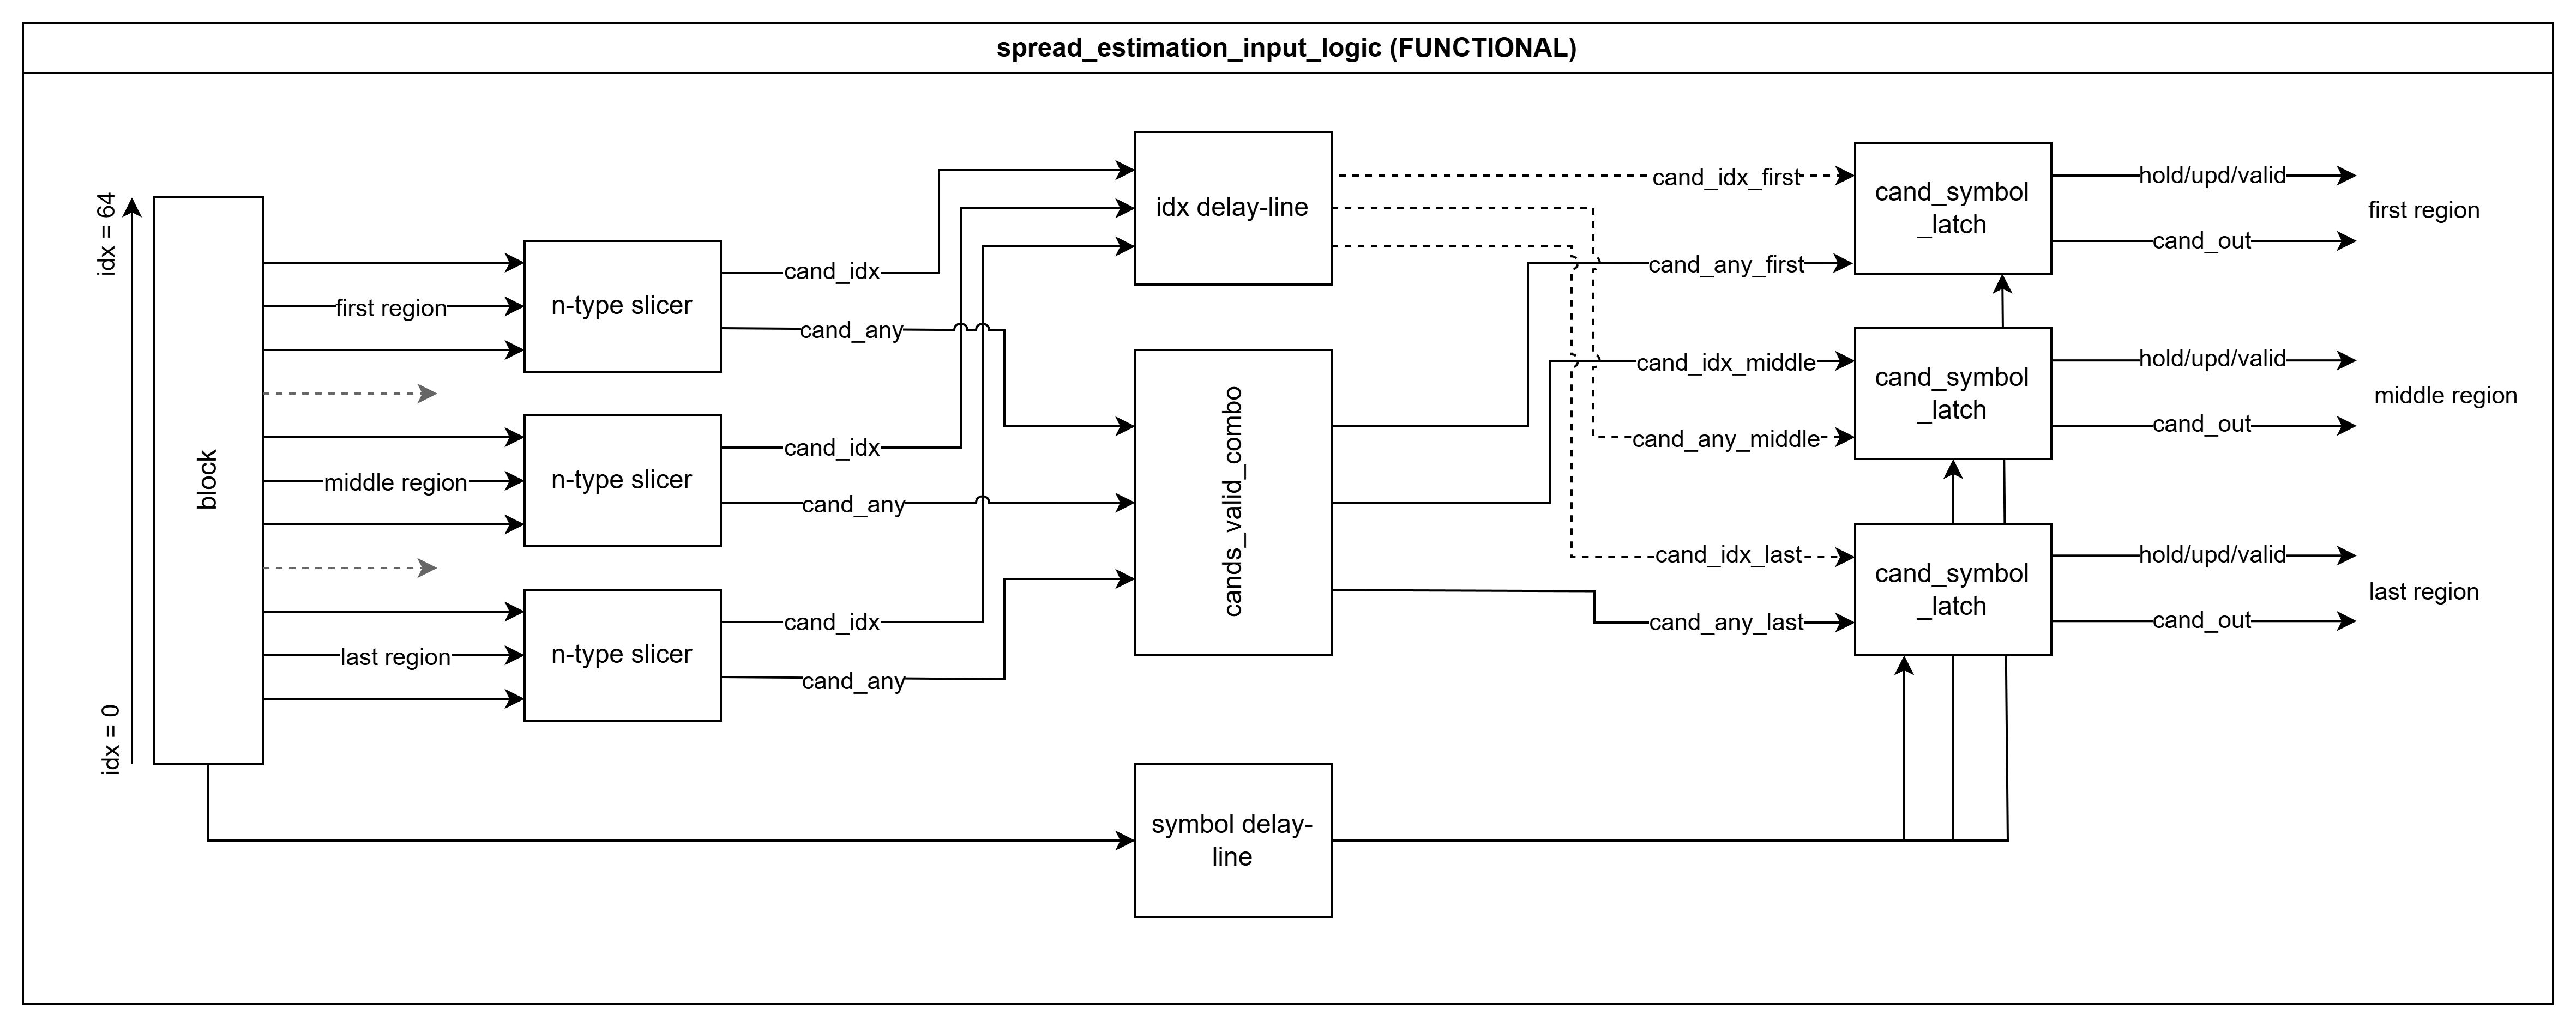
\includegraphics[width=1\linewidth]{figures/SE_input_logic_functional.png}
% \caption{Functional diagram of the SE input selector }
% \label{fig:SE_input_selector_functional}
% \end{figure}

% As input, it takes the whole block of symbols $ \bar r $, and outputs the candidate symbols $ x,y,z $ for the first, middle and last region of the block.

% This happens in 3 steps:
% \begin{enumerate}
%     \item locate which symbols in the \textit{first, middle \& last} regions are suitable candidates.
%     \item check for a suitable combination of \textit{first, middle \& last} candidates.
%     \item latch or update the output of these combinations to the spread and sign estimators.
% \end{enumerate}
% These steps are fullfiled respectively by the \textit{n-type slicer}, \textit{cands\_valid\_combo} , and \textit{cand\_symbol\_latch} module. 

% Each region of the block gets its own \textit{n-type slicer}. This module takes 3 symbols. The index 
% of the first available symbol that lies in the inner or outer circle \todo{explain somewhere what this criteria entails}
% is returned via the \textit{cand\_idx} bus. If no candidates are available, the \textit{cands\_any} flag is set to '0'. 

% Next, the \textit{cands\_valid\_combo} looks at the \textit{cands\_any} flags from each region, and only
% allows them to pass through if 2 or more regions have a candidate symbol. Otherwise, the single set flag is lowered. 
% This is to avoid wrong estimations \todo{explain more why, perhaps in algorithm explanation}. 

% These filtered flags are sent to the final module, the \textit{cand\_symbol\_latch}. It looks at every regions
% \textit{cands\_any} flag. If this flag are set, this module will output the symbol corresponding with that regions
% \textit{cand\_idx} from the input block of symbols \todo{important, maybe word better}. This also raises the \textit{update} flag, otherwise the \textit{hold} flag is raised.

% % \subsubsection{Data flow}
% % nothing special to say here?

% \subsubsection{Timing flow}
% The \textit{n-type slicer} takes two cycles to complete its decision and register it to the output of the module.
% Next, the \textit{cands\_valid\_combo} also takes one cycle to render its output of the \textit{cands\_any} flags stable. 

% Because the \textit{cand\_symbol\_latch} module assumes temporal consistency from its inputs (i.e. the block of symbols and the candidate
% indexes and their valid flags), a delay module needs to be added to match the largest latency link in the system. Symbols $ \bar r $ in the front
% of the input selector get delayed by 3 clockcycles to match the \textit{n-type slicer} $ + $  \textit{cands\_valid\_combo} latency. The 
% \textit{cand\_idx} busses get delayed with 1 cycle, matching the latency of the \textit{cands\_valid\_combo} module. 

% \begin{figure}[H]
% \centering
% 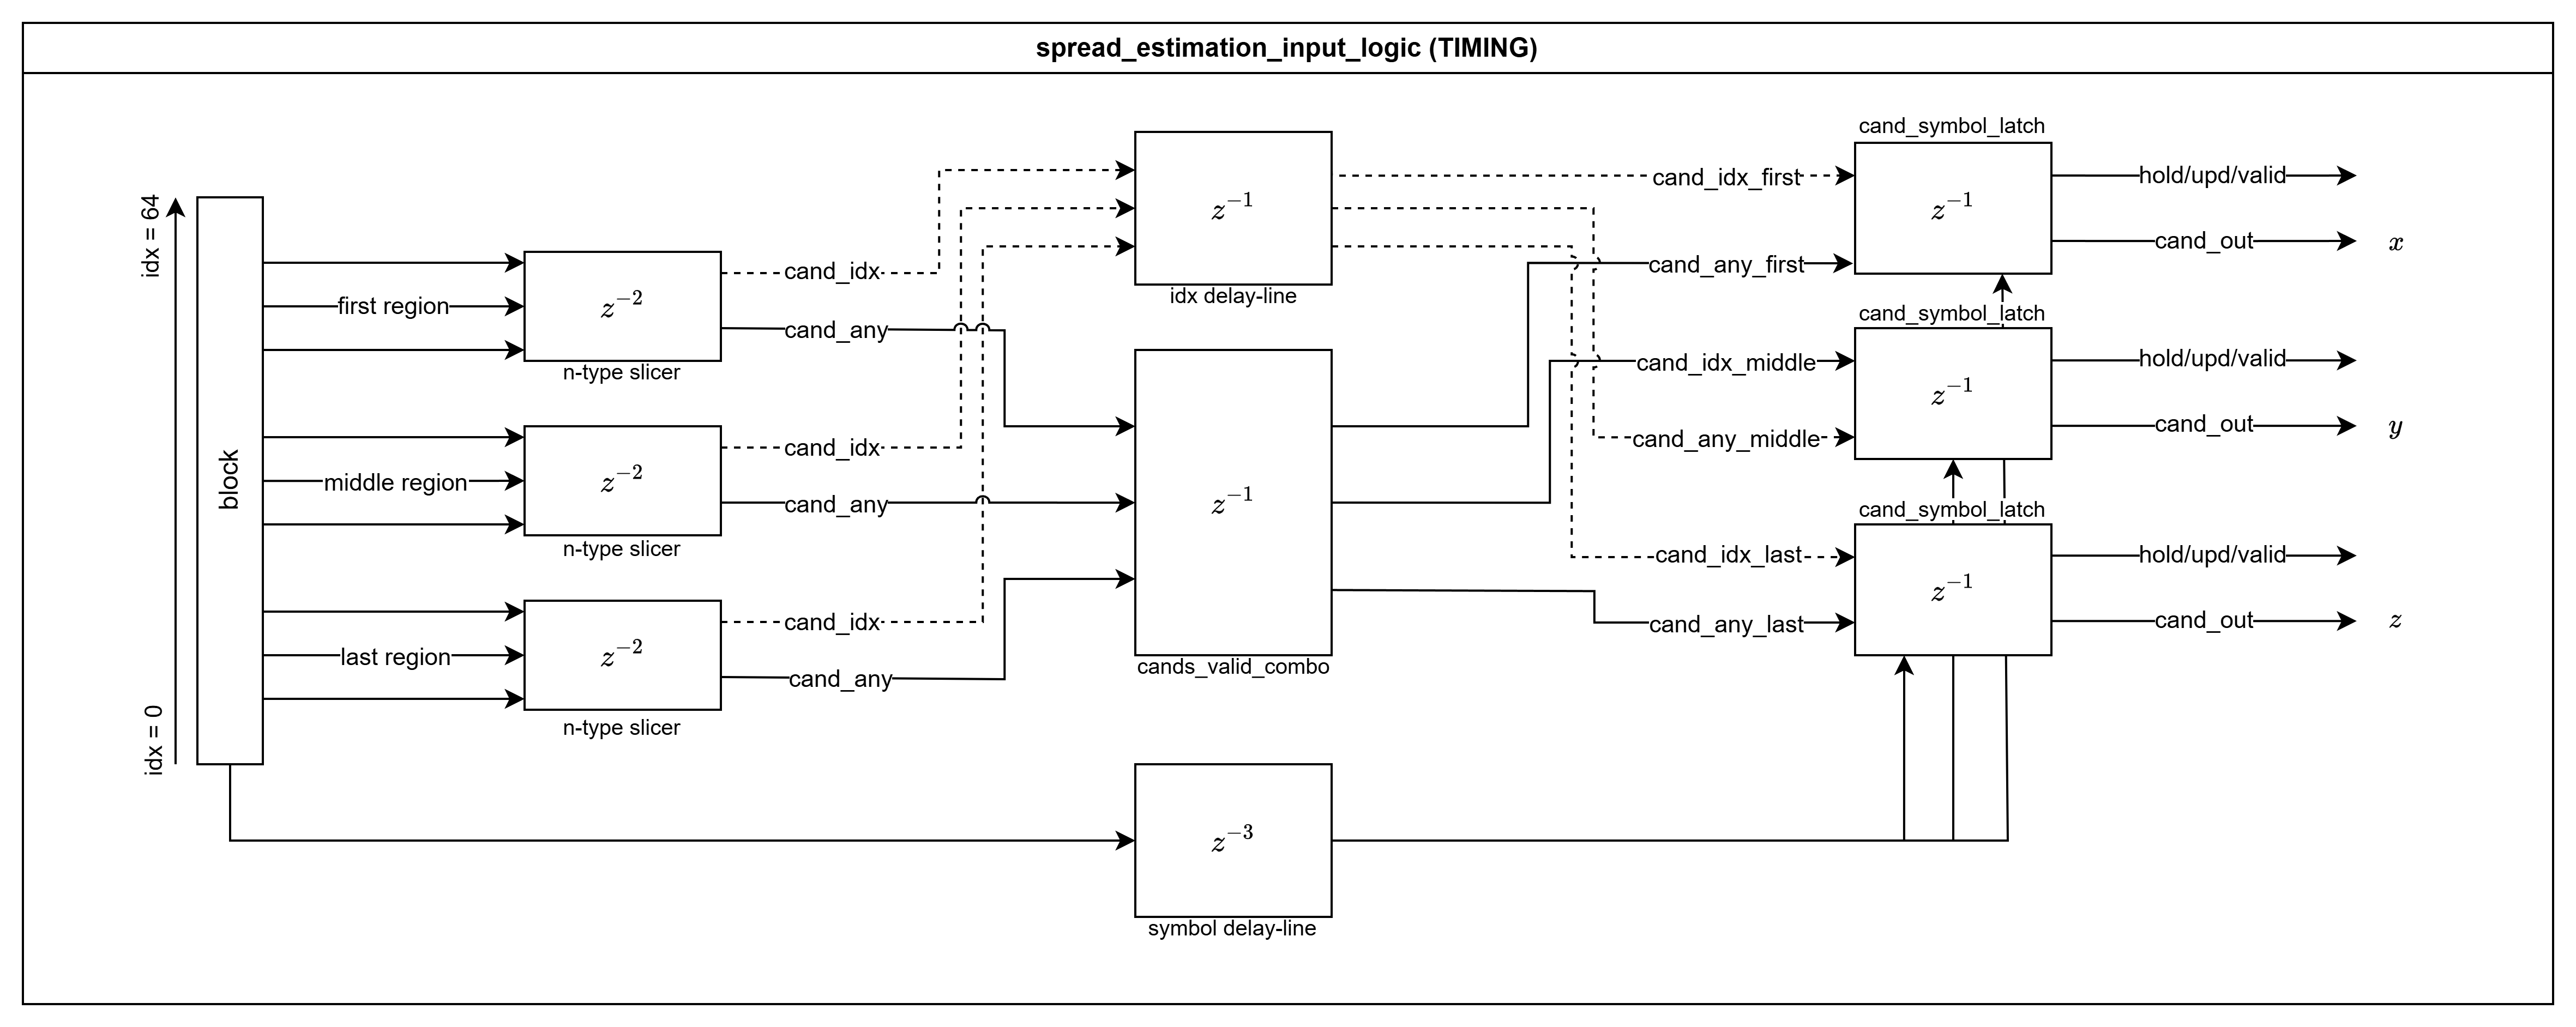
\includegraphics[width=1\linewidth]{figures/SE_input_logic_timing.png}
% \caption{Timing flow diagram of the SE input selector }
% \label{fig:SE_input_selector_timing}
% \end{figure}

% Finally, the \textit{cand\_symbol\_latch} takes one cycle to complete the latching for updates symbols, thus, taking the  
% latency of the input selector to 4 total clockcycles. 

\subsection{Input selector}
\subsubsection{Functional operation}

As introduced in Section~\ref{input selector}, the spread and direction estimation blocks require a set of representative symbols from the 
input block. However, not all symbols are suitable for this purpose. Therefore, an input selection stage is required to extract valid 
candidate symbols from different regions of the block.

\begin{figure}[H]
\centering
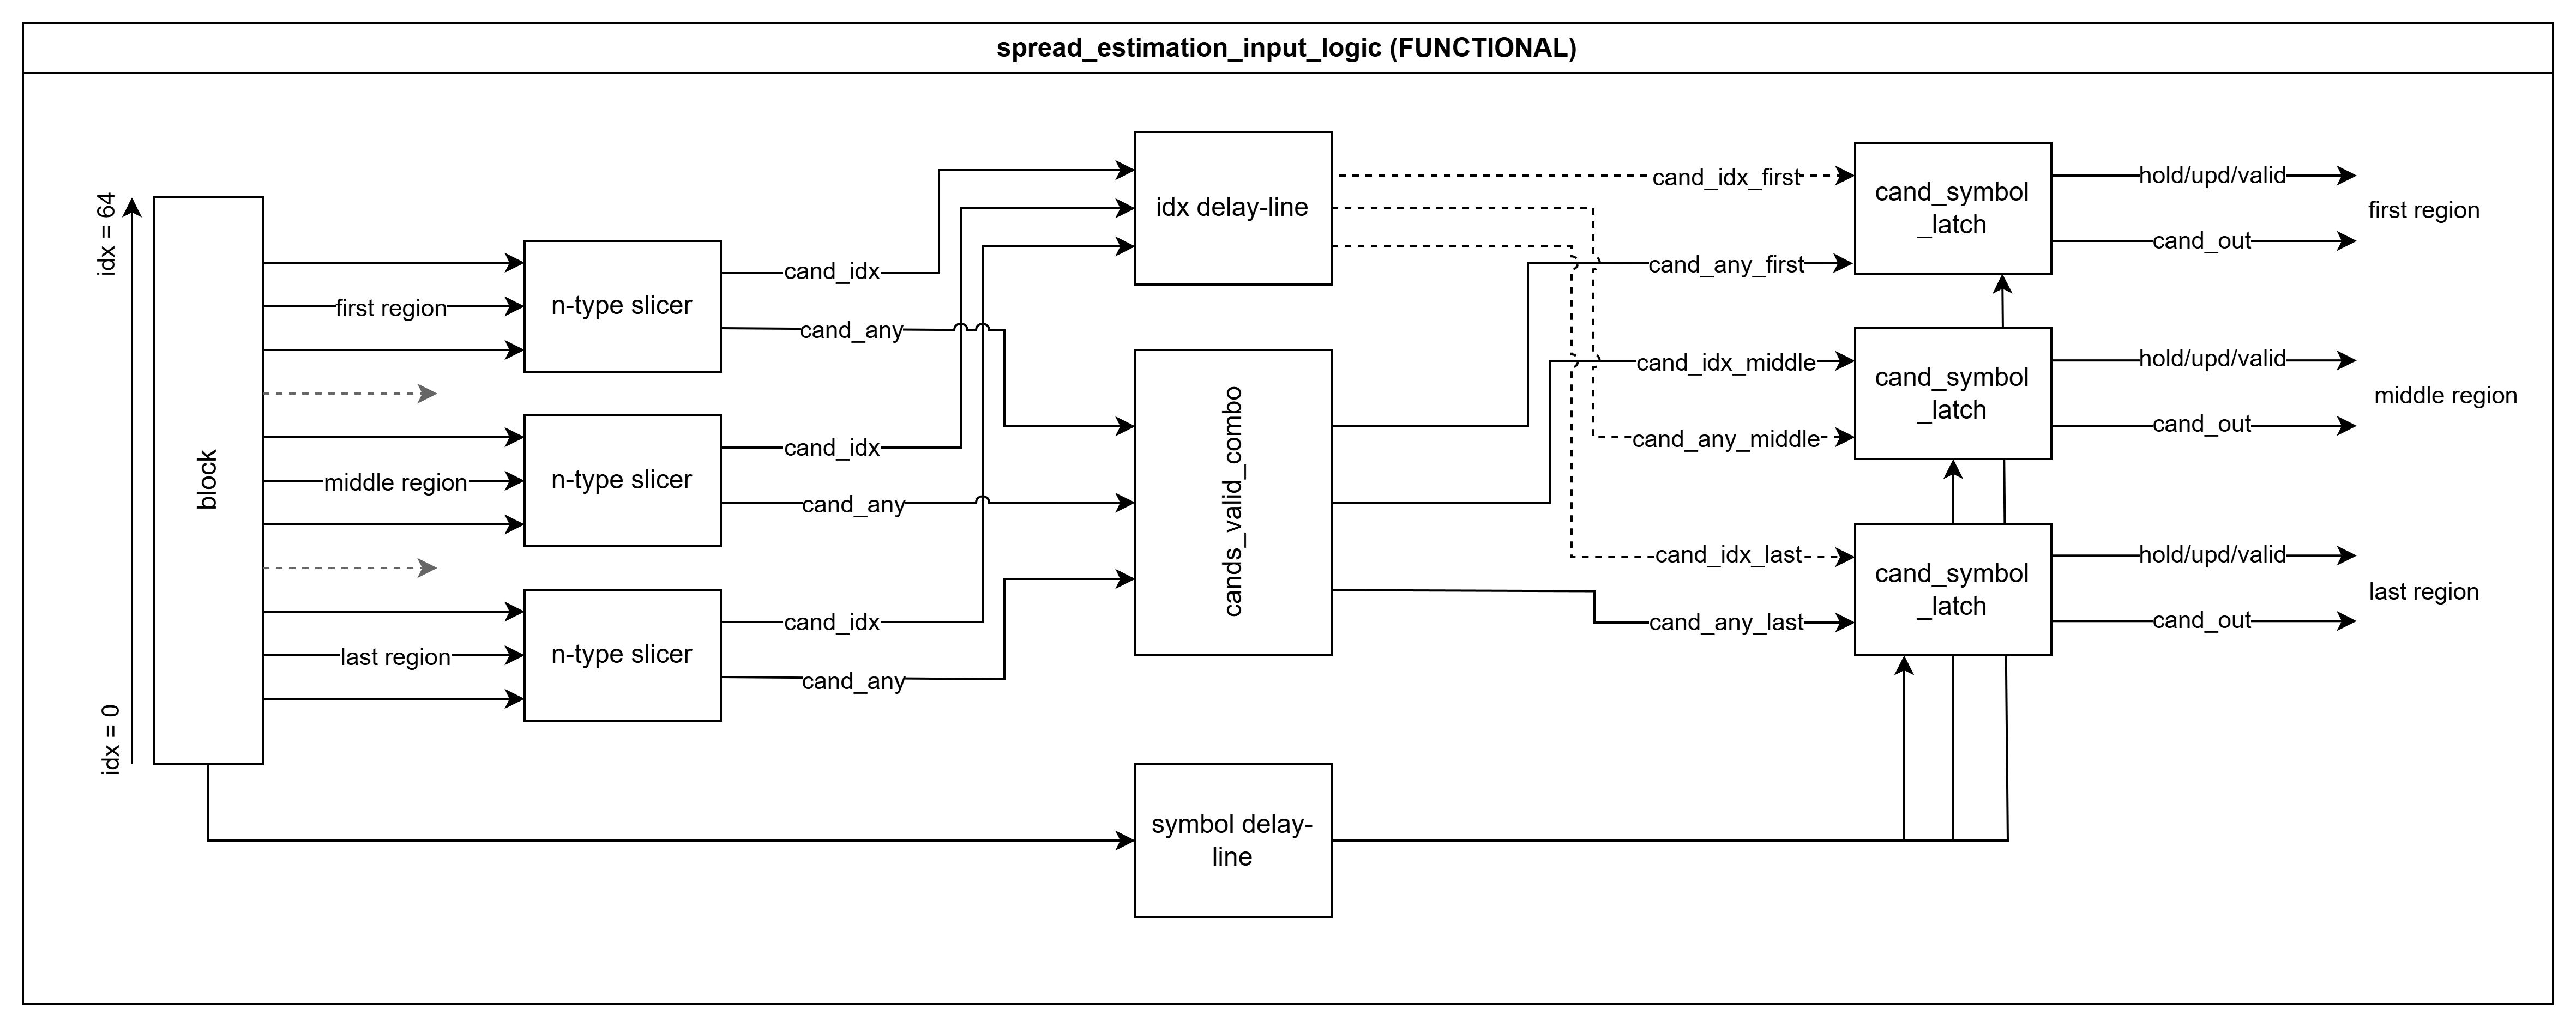
\includegraphics[width=1\linewidth]{figures/SE_input_logic_functional.png}
\caption{Functional diagram of the SE input selector}
\label{fig:SE_input_selector_functional}
\end{figure}

The input selector operates on the full block of received symbols $ \bar{r} $, and outputs three candidate symbols $x$, $y$, and $z$, 
corresponding to the first, middle, and last regions of the block, respectively. These candidates are subsequently used for spread and
direction estimation.
\\\\
The selection process consists of three sequential steps:

\begin{enumerate}
    \item Identification of valid candidate symbols within each region of the block.
    \item Validation of the combination of candidates across regions.
    \item Latching or updating of the selected symbols for further processing.
\end{enumerate}

These steps are implemented by the \textit{n-type slicer}, \textit{cands\_valid\_combo}, and \textit{cand\_symbol\_latch} modules, respectively.
\\\\
Each region (first, middle, last) is processed by an independent \textit{n-type slicer}. 
This module evaluates a small subset of symbols (three in this implementation) and determines 
whether a suitable candidate is present. A symbol is considered valid if it lies on the inner or 
outer ring of the constellation, which ensures reliable spread estimation (this criterion is further 
elaborated in the algorithmic description of the spread estimator). The index of the first valid symbol 
is returned via the \textit{cand\_idx} bus. If no valid candidate is found, the \textit{cands\_any} flag is deasserted.
\\\\
The \textit{cands\_valid\_combo} module evaluates the availability of candidates across the three regions.
A valid combination is only accepted if at least two regions provide a candidate symbol. If this condition is not met,
 all candidate flags are suppressed. This constraint reduces the likelihood of unreliable spread or direction estimates, 
 which would otherwise arise from insufficient spatial information within the block.
\\\\
Finally, the \textit{cand\_symbol\_latch} module selects and outputs the candidate symbols. For each region where the 
\textit{cands\_any} flag is asserted, the corresponding symbol is extracted from the input block using the provided 
\textit{cand\_idx}. If valid candidates are present, the outputs are updated and the \textit{update} signal is asserted. 
Otherwise, the previous outputs are retained and the \textit{hold} signal is asserted. In this way, consistency is maintained 
when no valid candidate combination is available.

\subsubsection{Timing flow}

The timing behaviour of the input selector is illustrated in Figure~\ref{fig:SE_input_selector_timing}.
\\\\
The \textit{n-type slicer} requires two clock cycles to determine and register a valid candidate index. The subsequent 
\textit{cands\_valid\_combo} stage introduces an additional cycle to produce stable validity signals.
\\\\
To ensure correct operation of the \textit{cand\_symbol\_latch}, all inputs must be temporally aligned. In particular, 
the candidate indices and their corresponding validity flags must be synchronized with the original input symbols. To achieve this, 
delay elements are inserted in the data path. The input symbol block $ \bar{r} $ is delayed by three clock cycles, matching the 
combined latency of the slicer and combination stages. The \textit{cand\_idx} signals are delayed by one cycle to align with the 
output of the \textit{cands\_valid\_combo} module.

\begin{figure}[H]
\centering
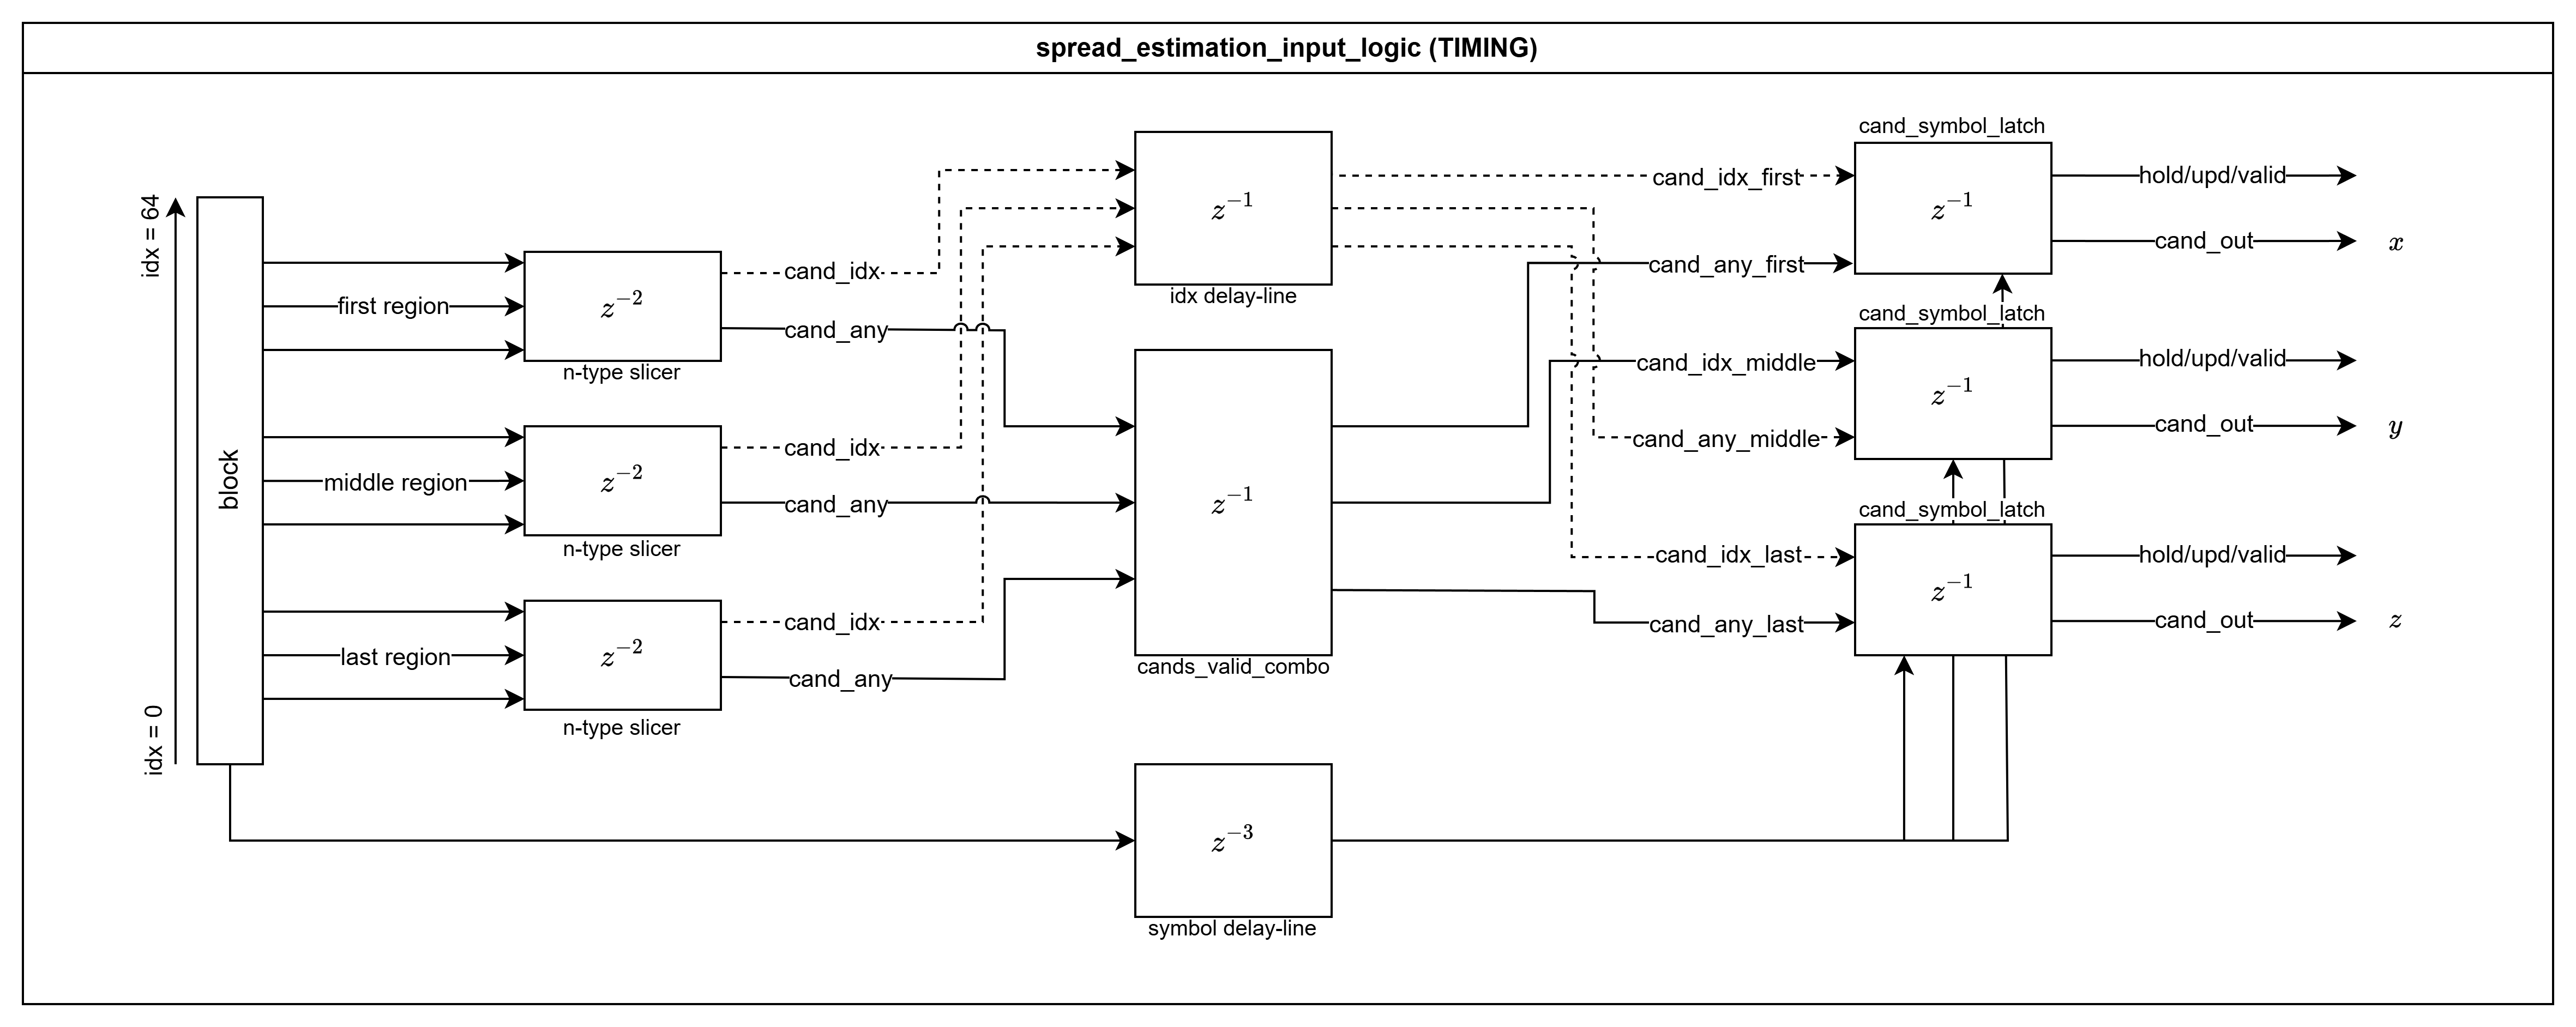
\includegraphics[width=1\linewidth]{figures/SE_input_logic_timing.png}
\caption{Timing flow diagram of the SE input selector}
\label{fig:SE_input_selector_timing}
\end{figure}

The \textit{cand\_symbol\_latch} itself introduces one additional clock cycle to register the selected symbols. 
As a result, the total latency of the input selector amounts to four clock cycles.

\subsection{Fourth-power I/Q calculators}
\subsubsection{Functional operation}
The fourth-power calculators are an important part of the system. The type of calculations needed
to perform a fourth-power on I/Q samples require multiplications, more of them than any other type of calculation
that needs to be done for the low-complexity carrier recovery system. 
\\\\

\subsubsection{Data flow}
\subsubsection{Timing flow}

\subsection{Spread estimation}
\subsubsection{Functional operation}
\begin{enumerate}
    \item compute dotproduct  
    \item compute denumerator (inner + outer flags go to radius LUT with as output inversed reciprocal multiplication factors) \todo{important, explain well!}
    \item multiplication of dotproduct with rec. mult. factor to produce $ \cos(|4\theta|) $. 
    \item $ \arccos $ LUT
\end{enumerate}

\subsubsection{Data flow}
\subsubsection{Timing flow}

\subsection{Sign estimation}
\subsubsection{Functional operation}
sign pair decider go to  first + middle or middle + last combination 
with that combo complex cross sign 

\subsubsection{Data flow}
\subsubsection{Timing flow}

\subsection{Filters}
% \subsubsection{Functional operation}
% \subsubsection{Data flow}
\subsubsection{Timing flow}







\section{Phase correction block}
\section{Top-level integration}



